\section{Wjets background in the signal region}
\label{app:WjetsInSignalRegion}

The distribution of the extrapolated W+jets background in the signal region, 
for each working point.

\begin{figure}[!t]
  \centering
    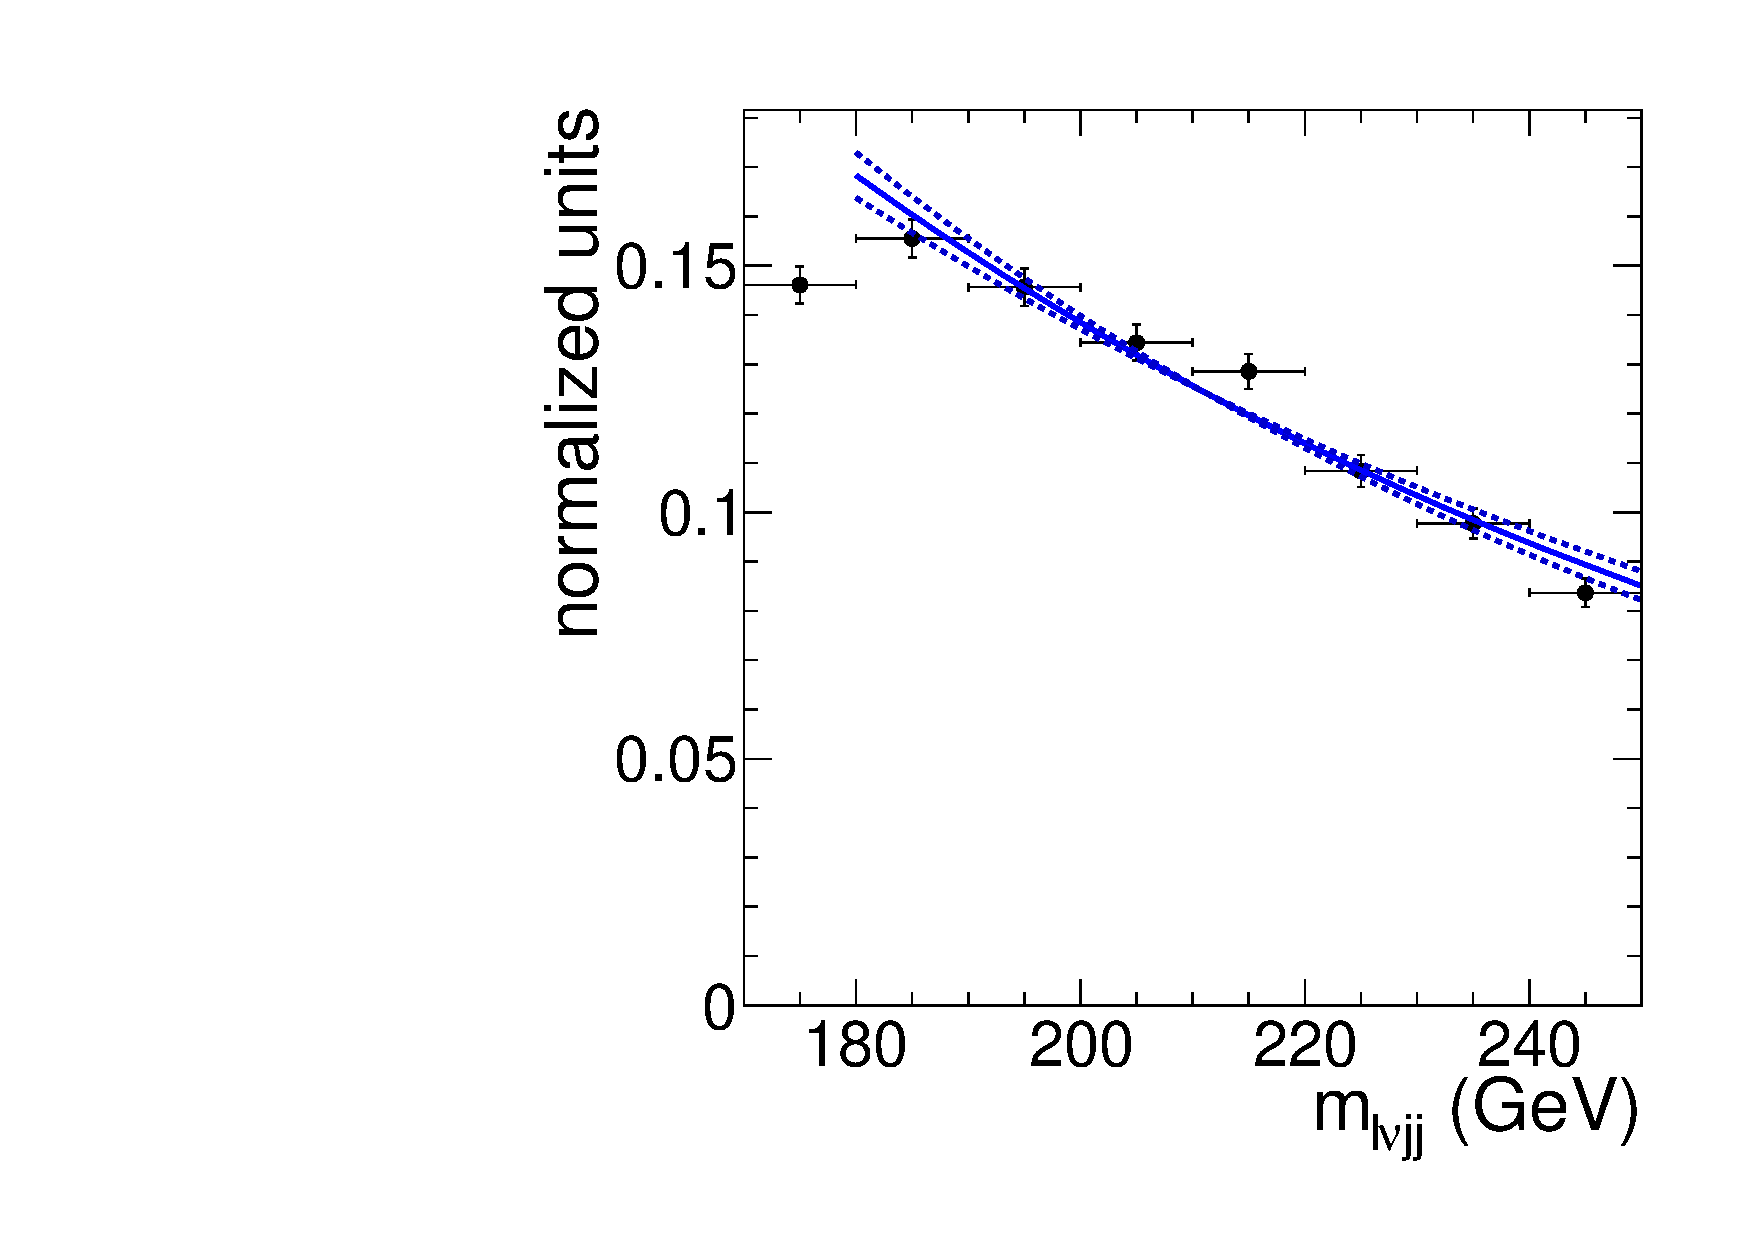
\includegraphics[width=0.49\textwidth]{plots/2012_WJetsShape/H170_Mlvjj_Electron_2jets_WpJShape.pdf}
    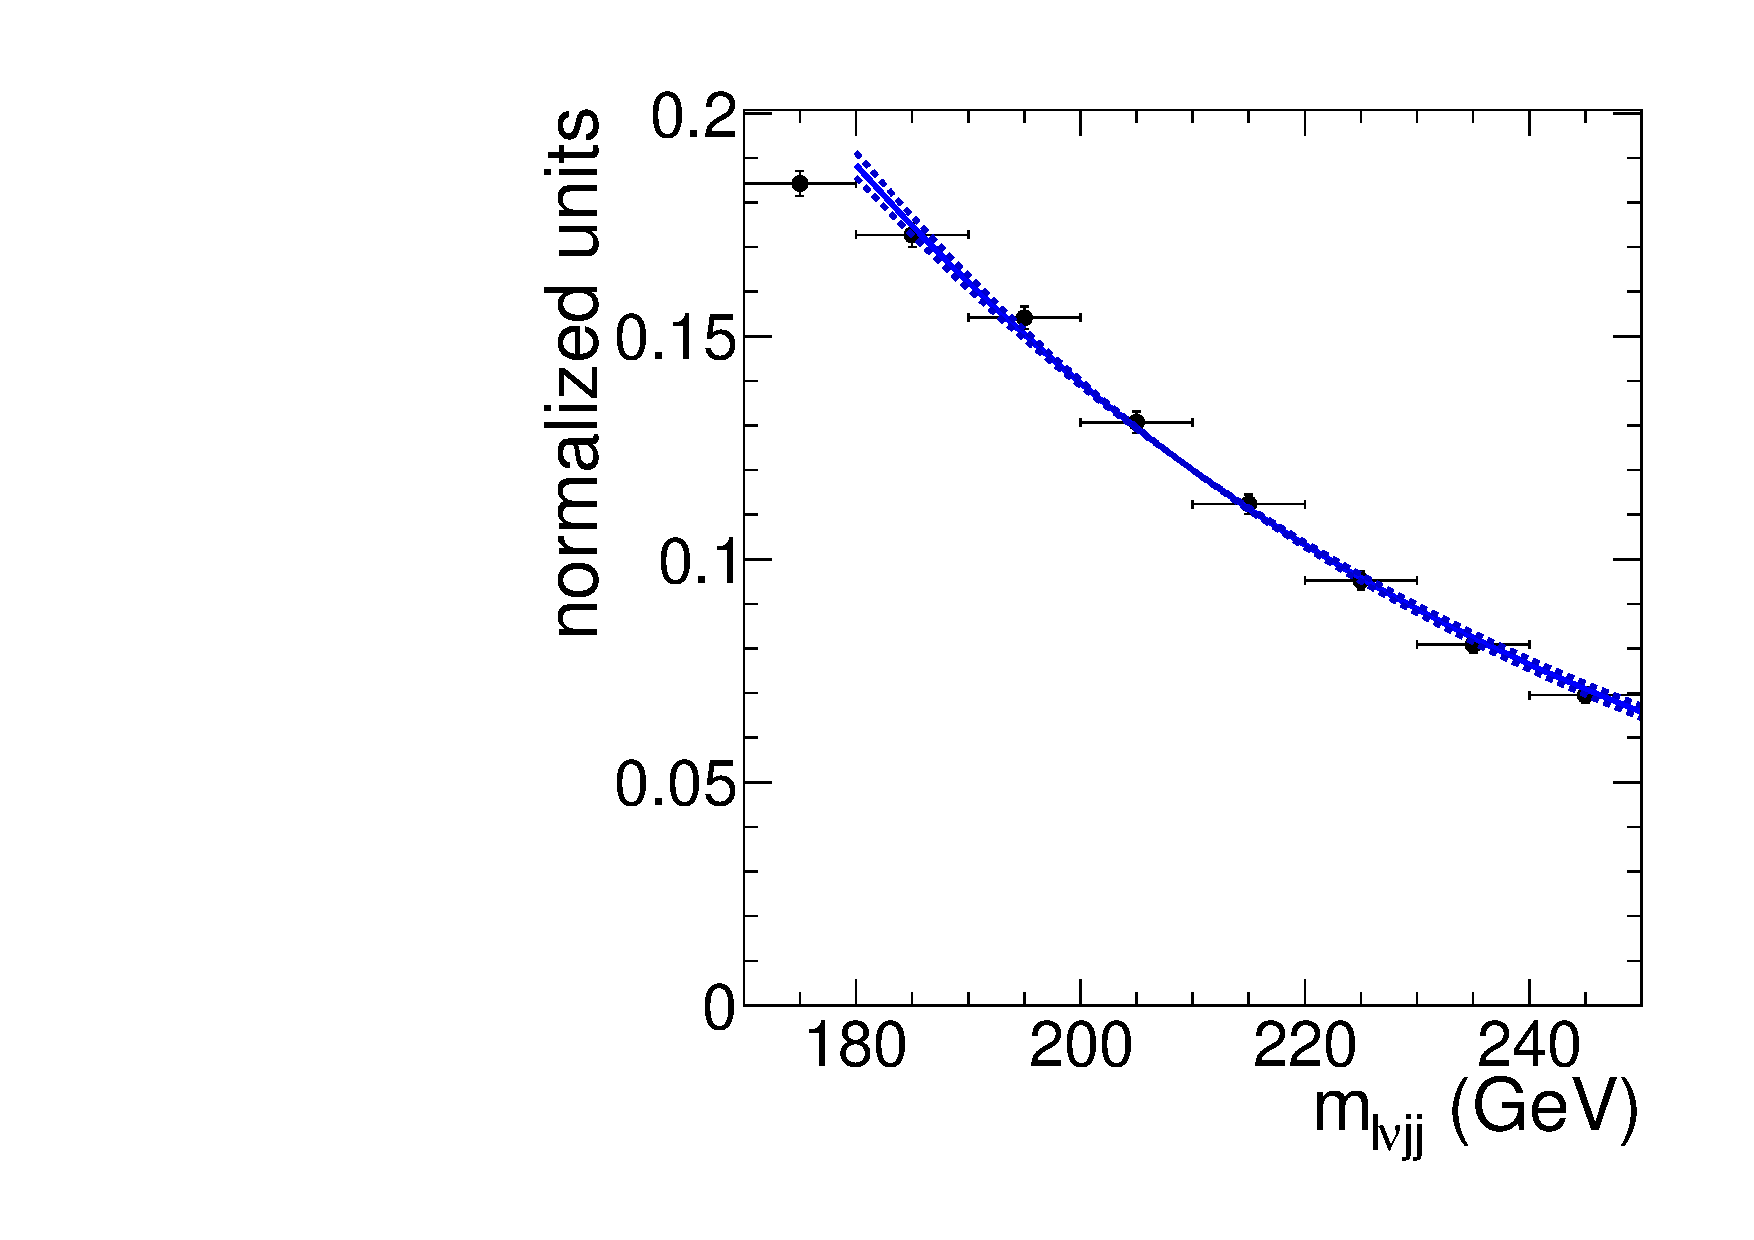
\includegraphics[width=0.49\textwidth]{plots/2012_WJetsShape/H170_Mlvjj_Muon_2jets_WpJShape.pdf}
    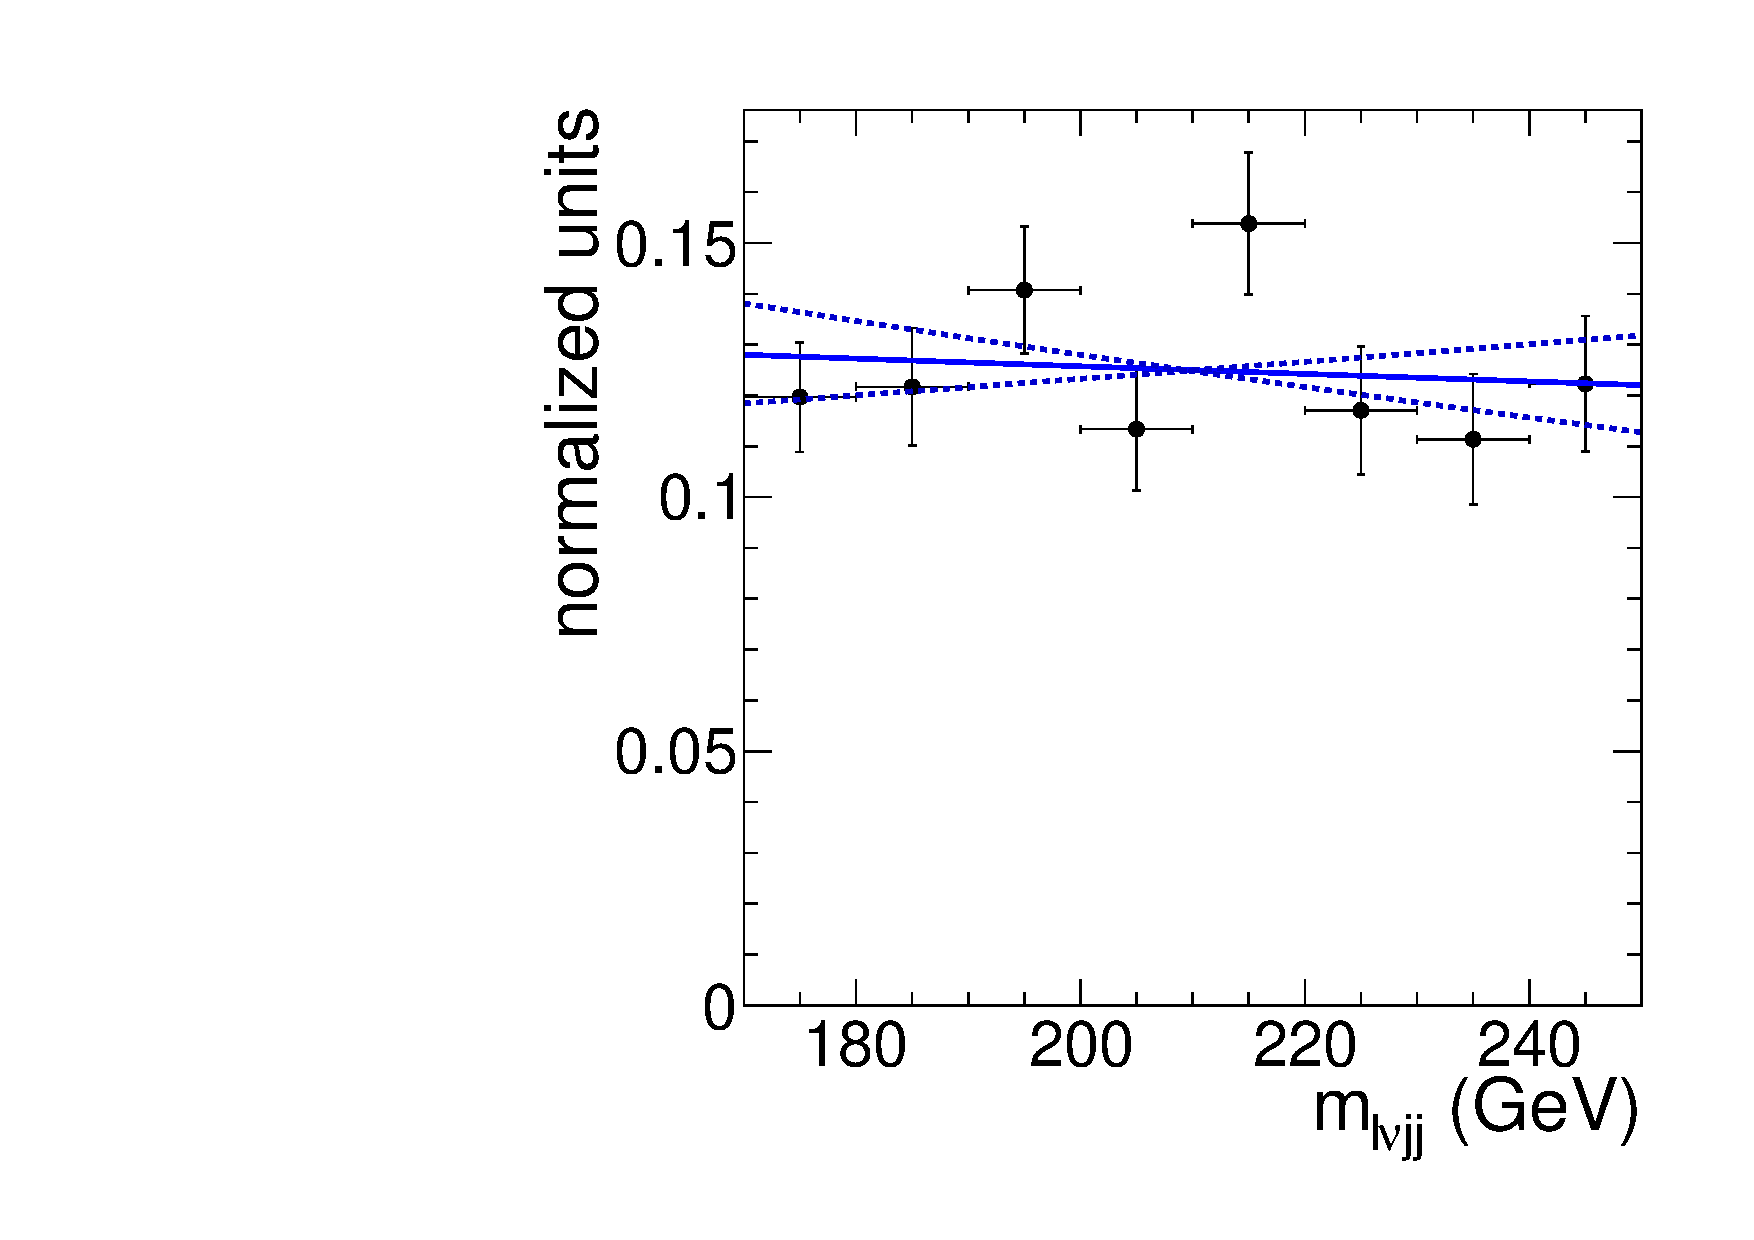
\includegraphics[width=0.49\textwidth]{plots/2012_WJetsShape/H170_Mlvjj_Electron_3jets_WpJShape.pdf}
    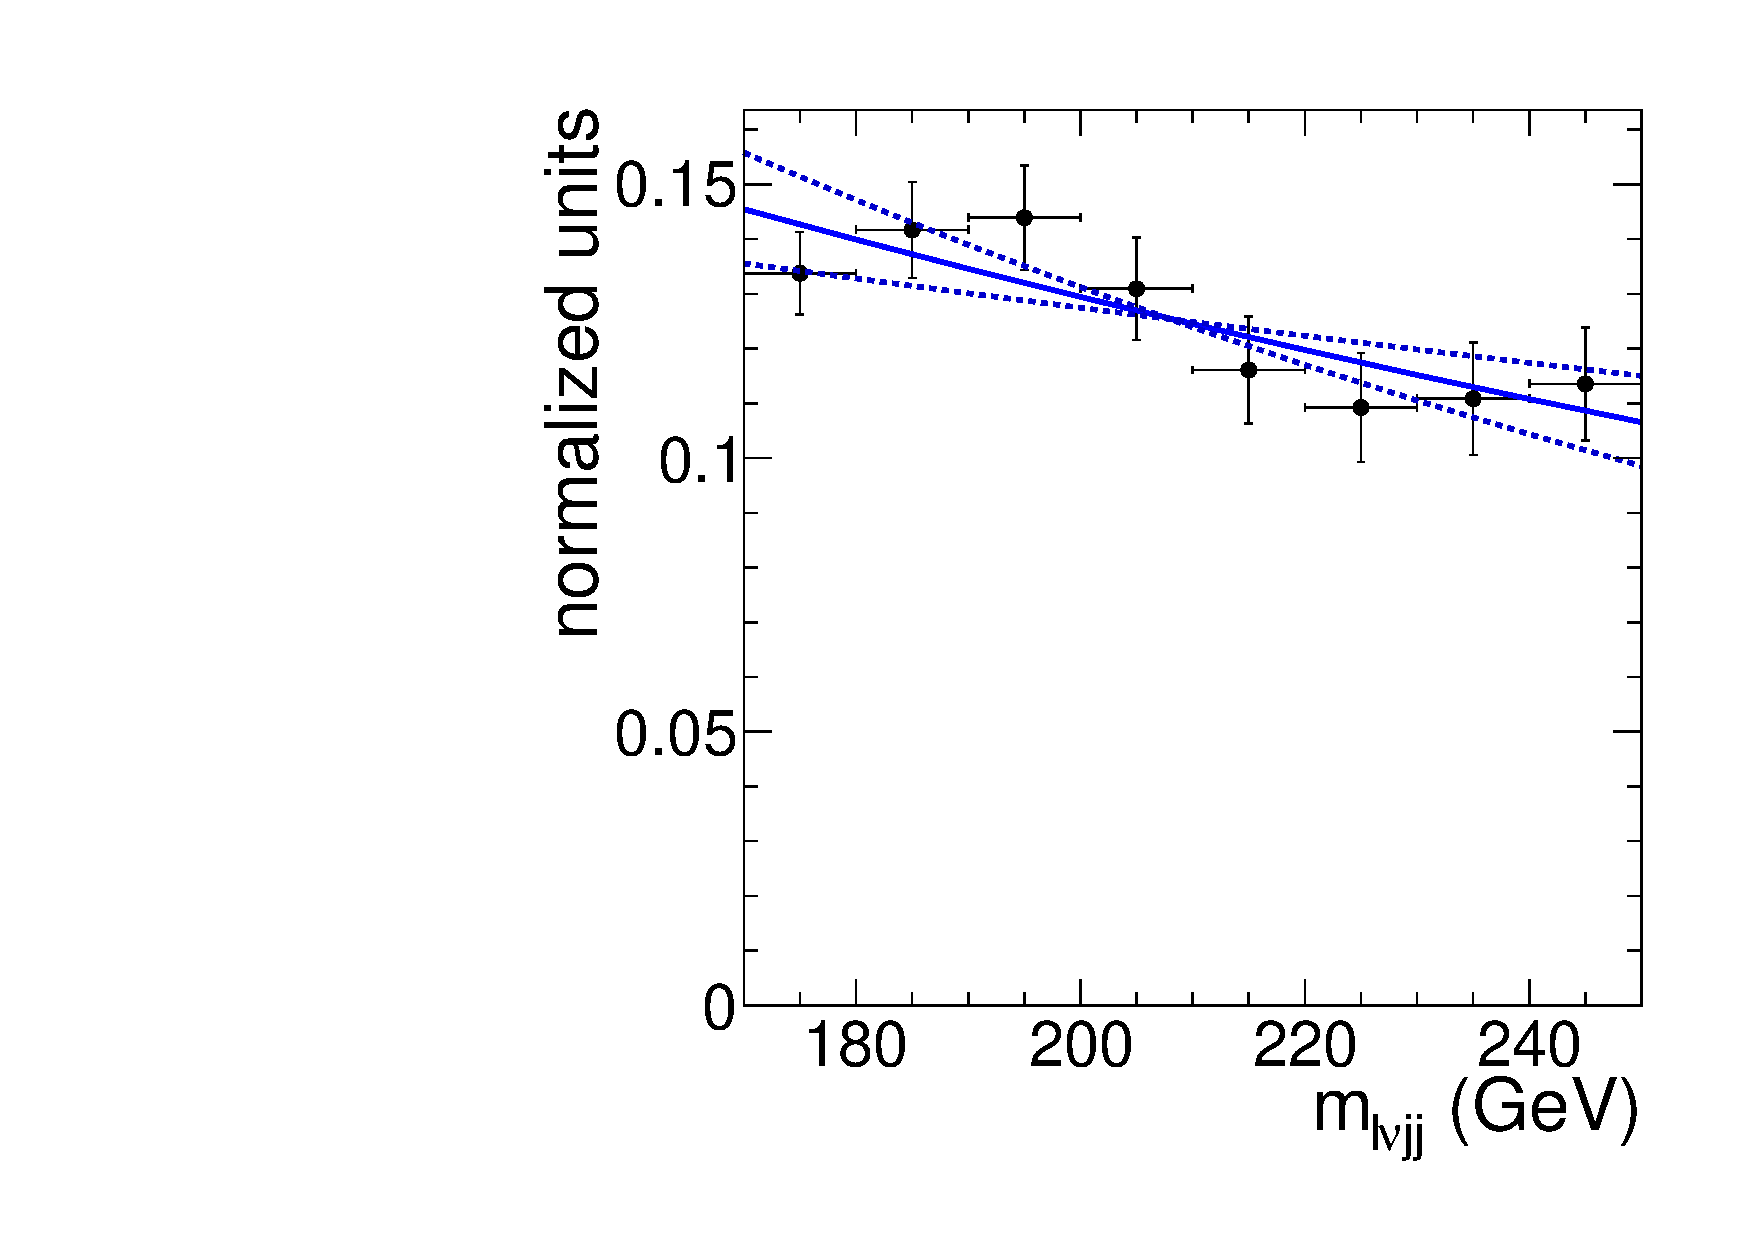
\includegraphics[width=0.49\textwidth]{plots/2012_WJetsShape/H170_Mlvjj_Muon_3jets_WpJShape.pdf}
  \caption{\label{fig:Wjets_dd_170}
  The distribution of the extrapolated background in the signal region
  is reported for the Higgs mass hypothesis of 170 GeV.
  On the top the 2 jets case, on the bottom the 3 jets case.
  Electrons are on the left, muons on the right.
  The points represent the extrapolated points, 
  while the red line shows the fitting function and the blue shaded band 
  the error from the fit.
    } 
\end{figure}
%
\begin{figure}[!t]
  \centering
    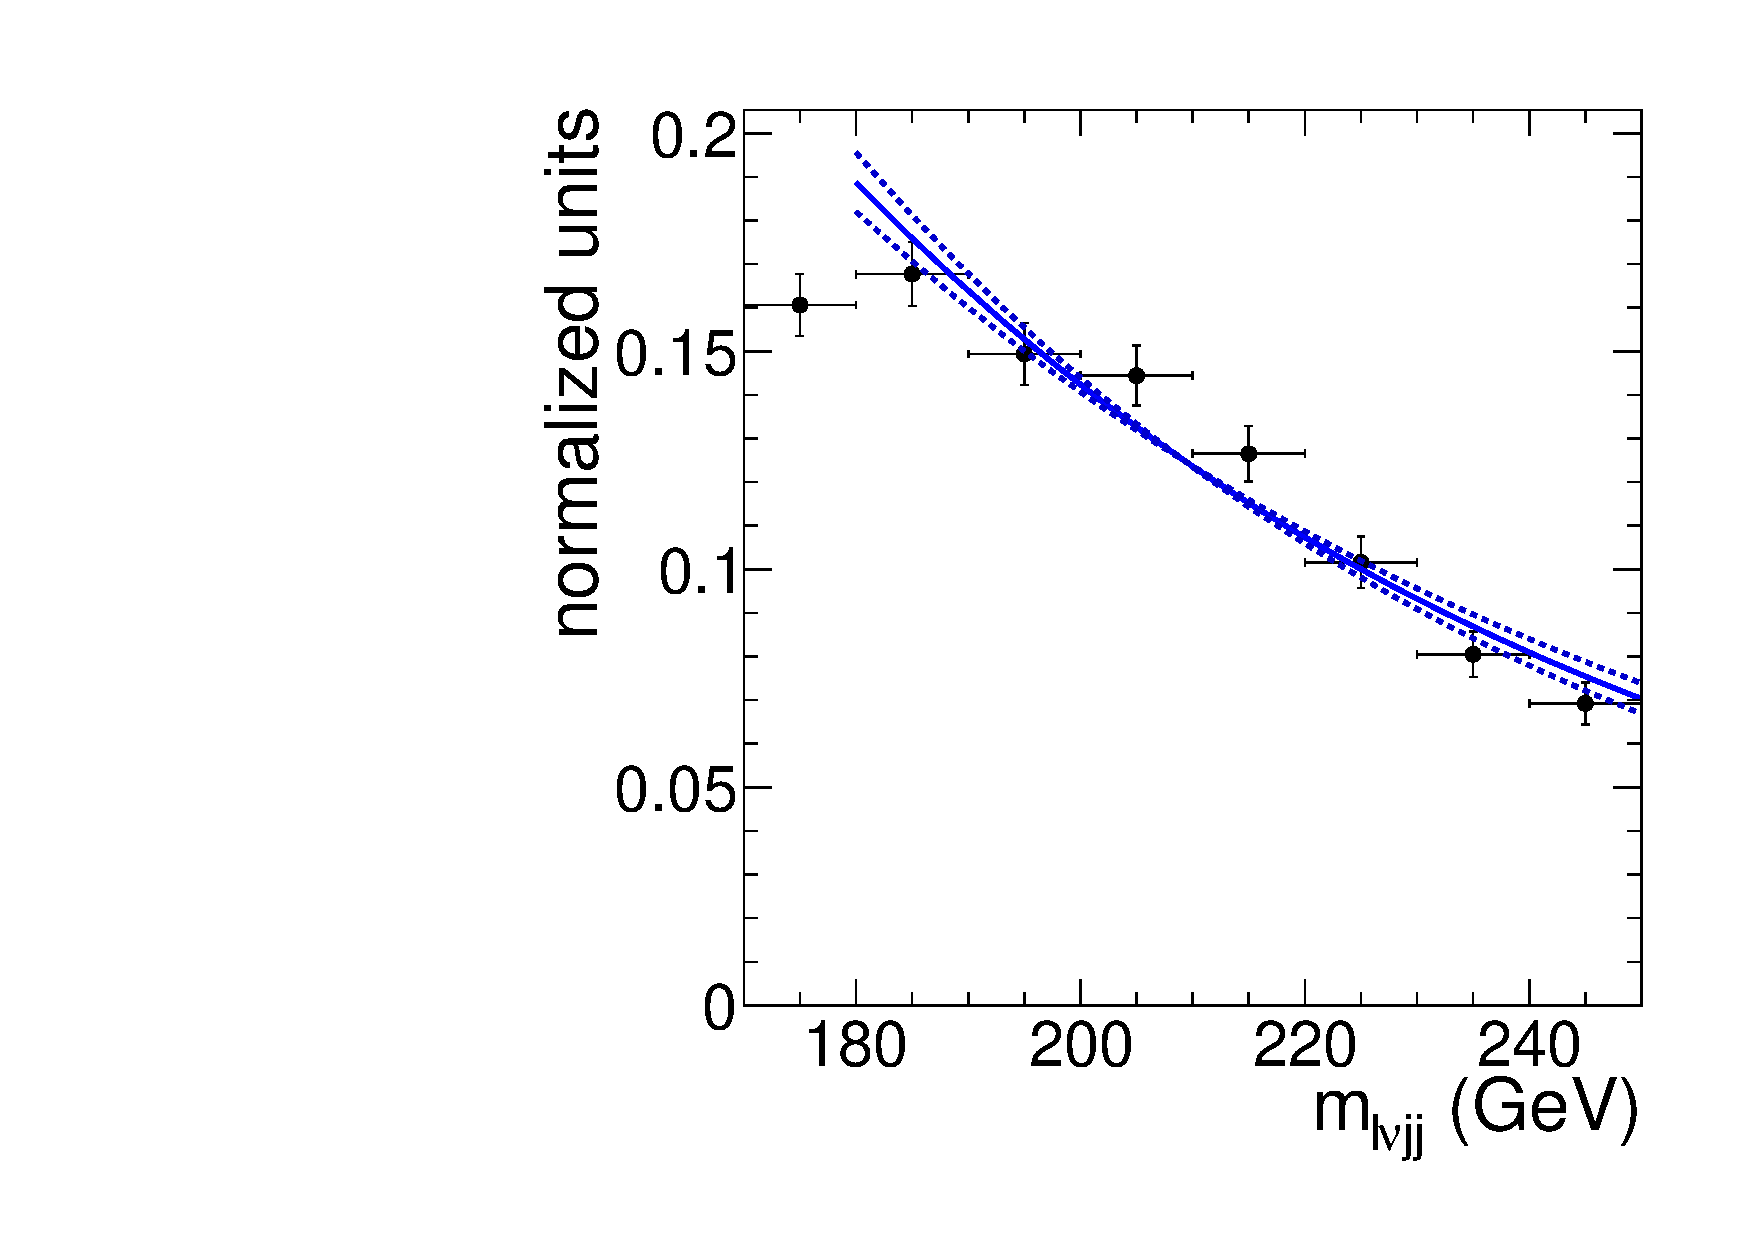
\includegraphics[width=0.49\textwidth]{plots/2012_WJetsShape/H180_Mlvjj_Electron_2jets_WpJShape.pdf}
    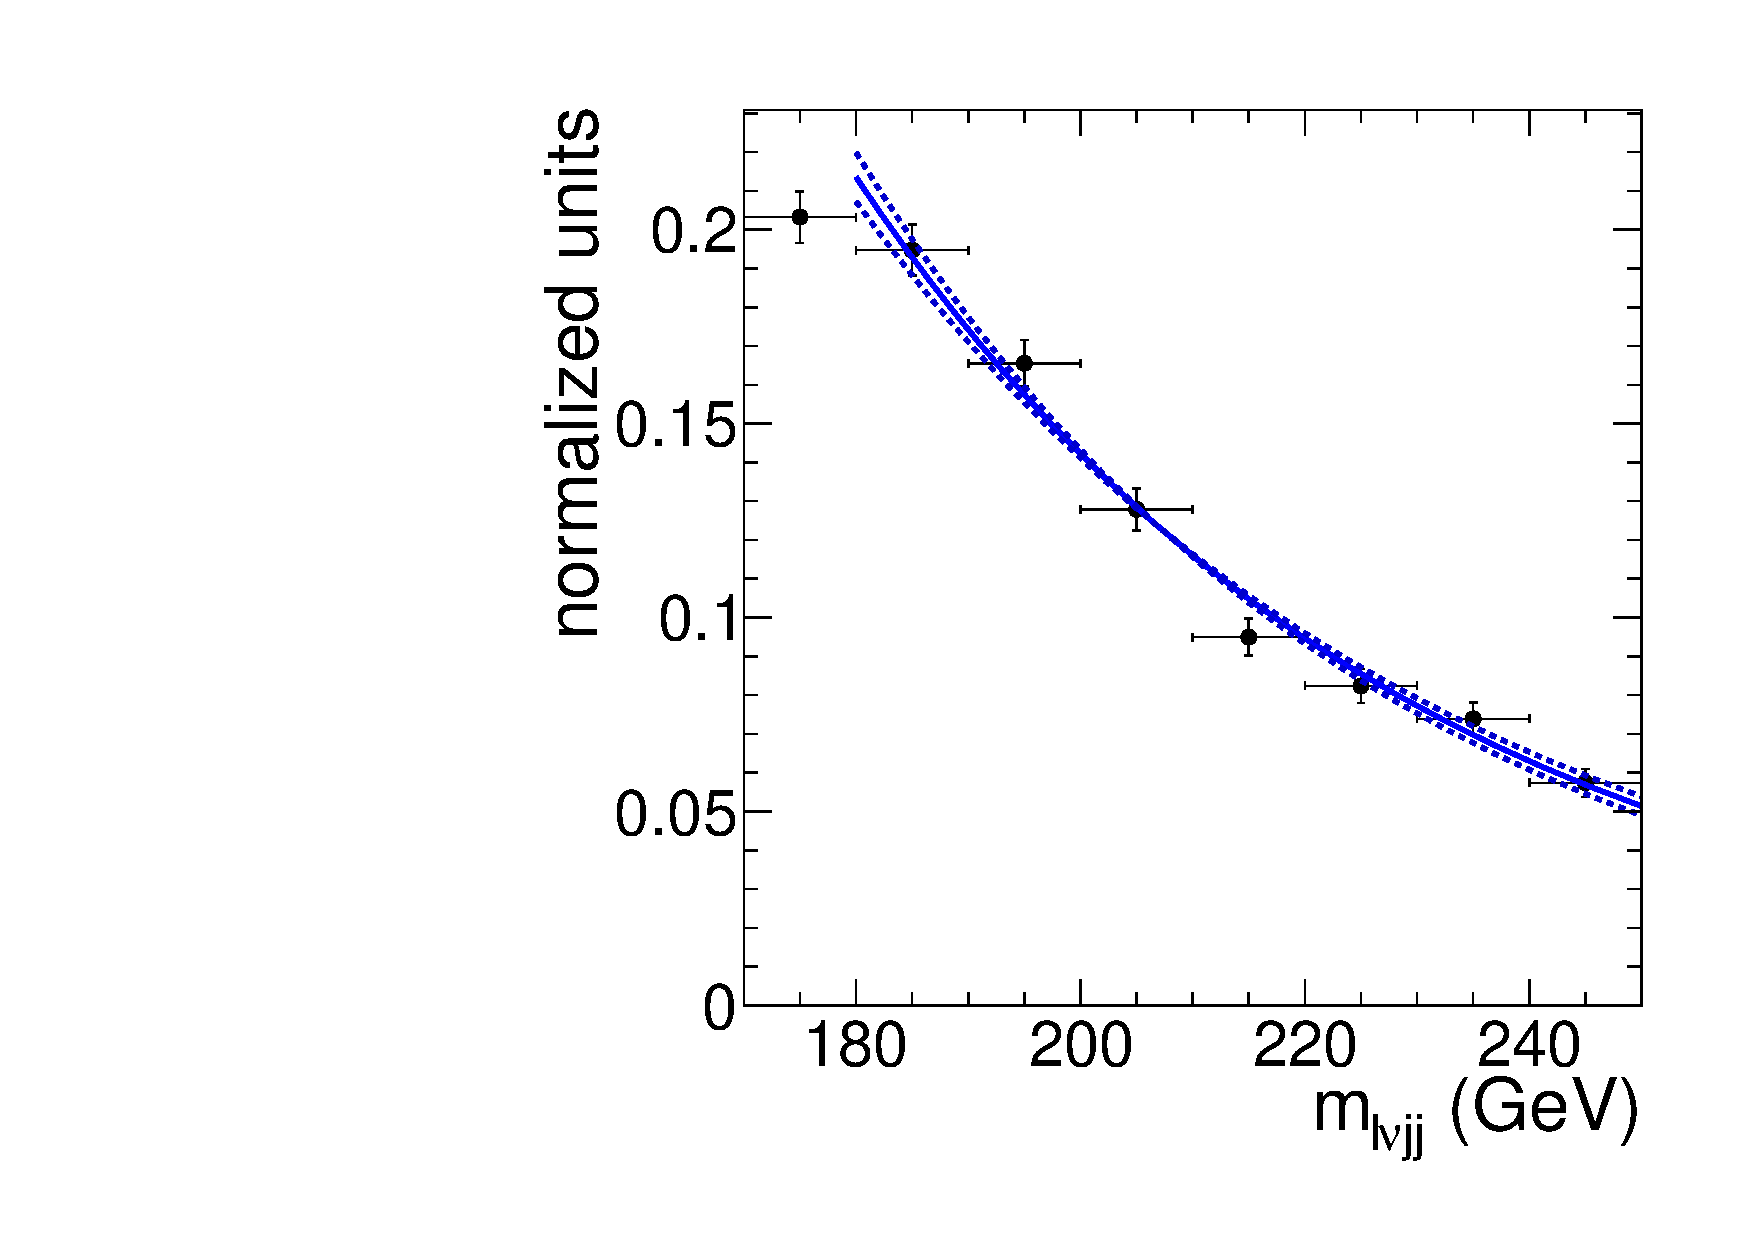
\includegraphics[width=0.49\textwidth]{plots/2012_WJetsShape/H180_Mlvjj_Muon_2jets_WpJShape.pdf}
    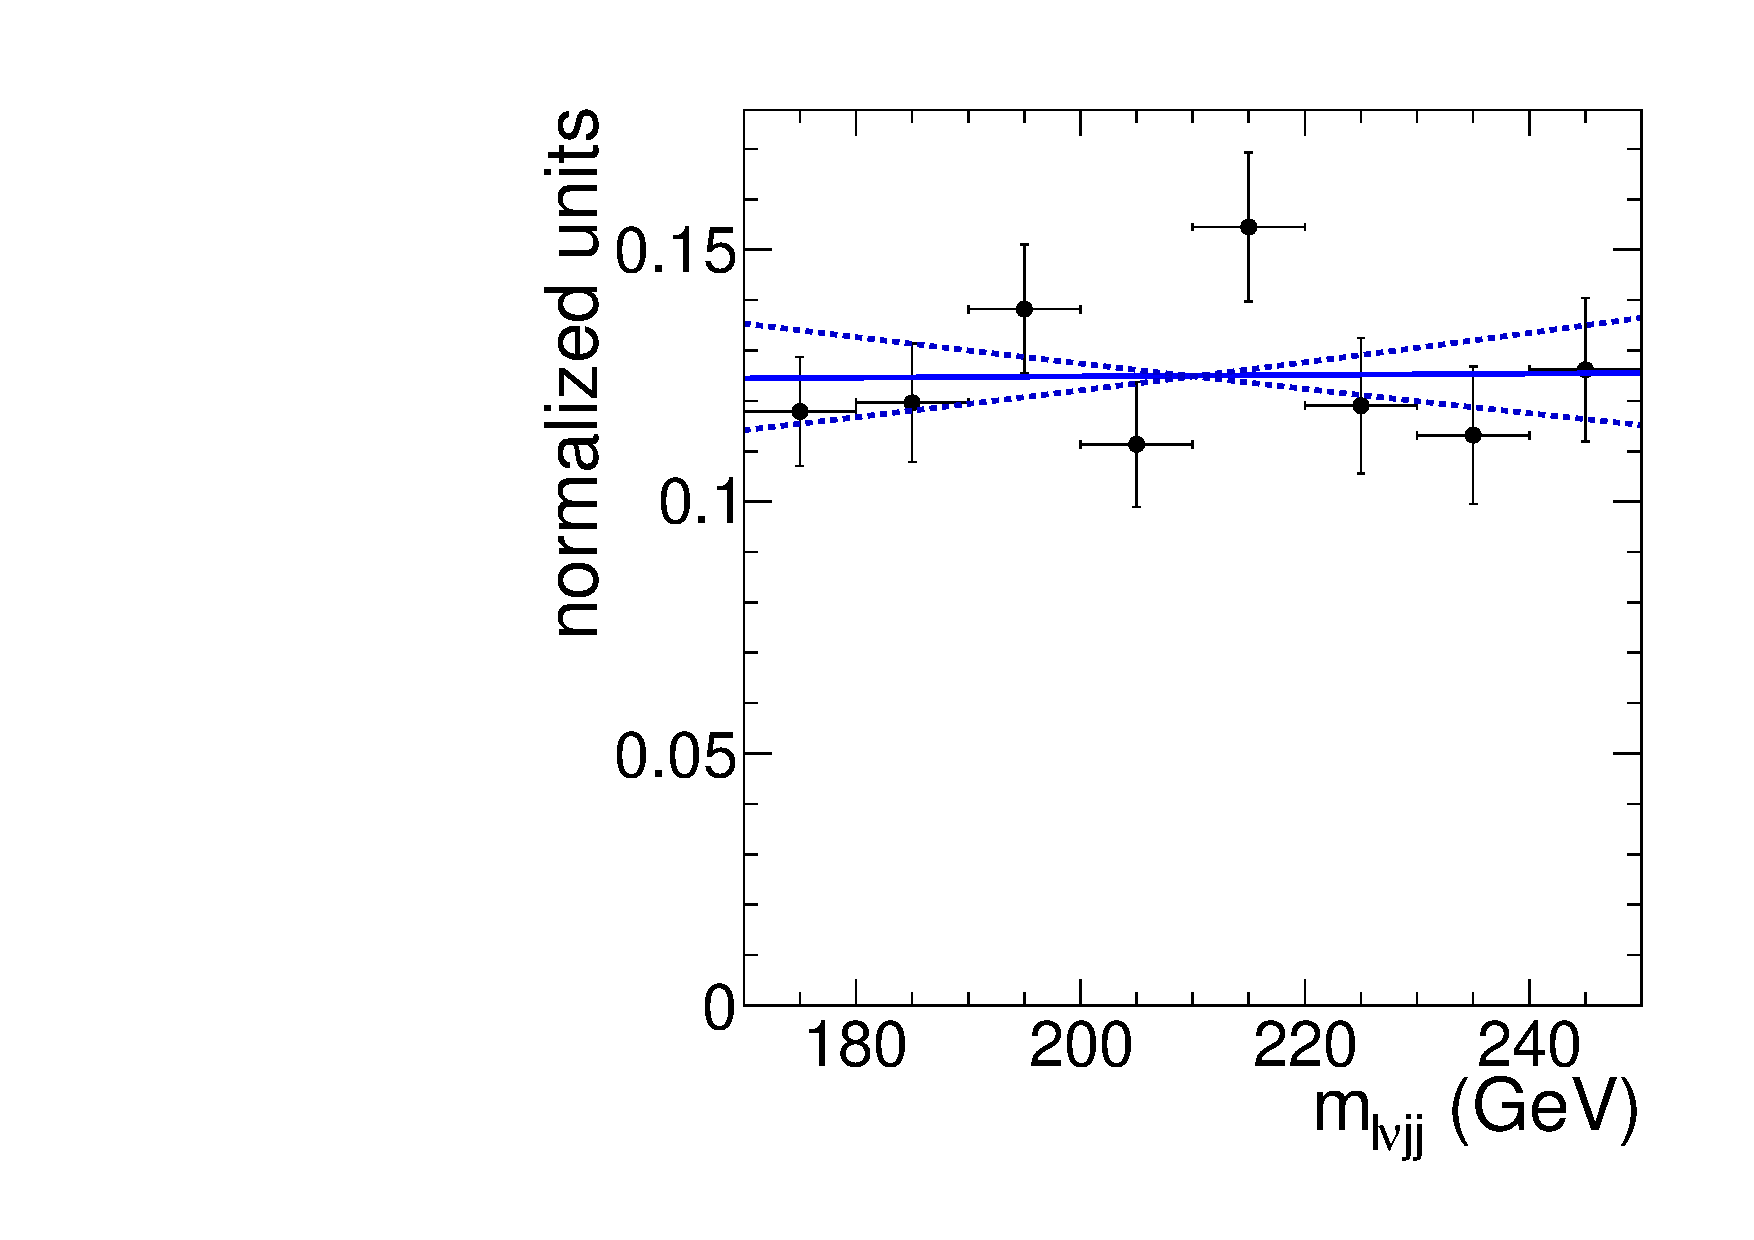
\includegraphics[width=0.49\textwidth]{plots/2012_WJetsShape/H180_Mlvjj_Electron_3jets_WpJShape.pdf}
    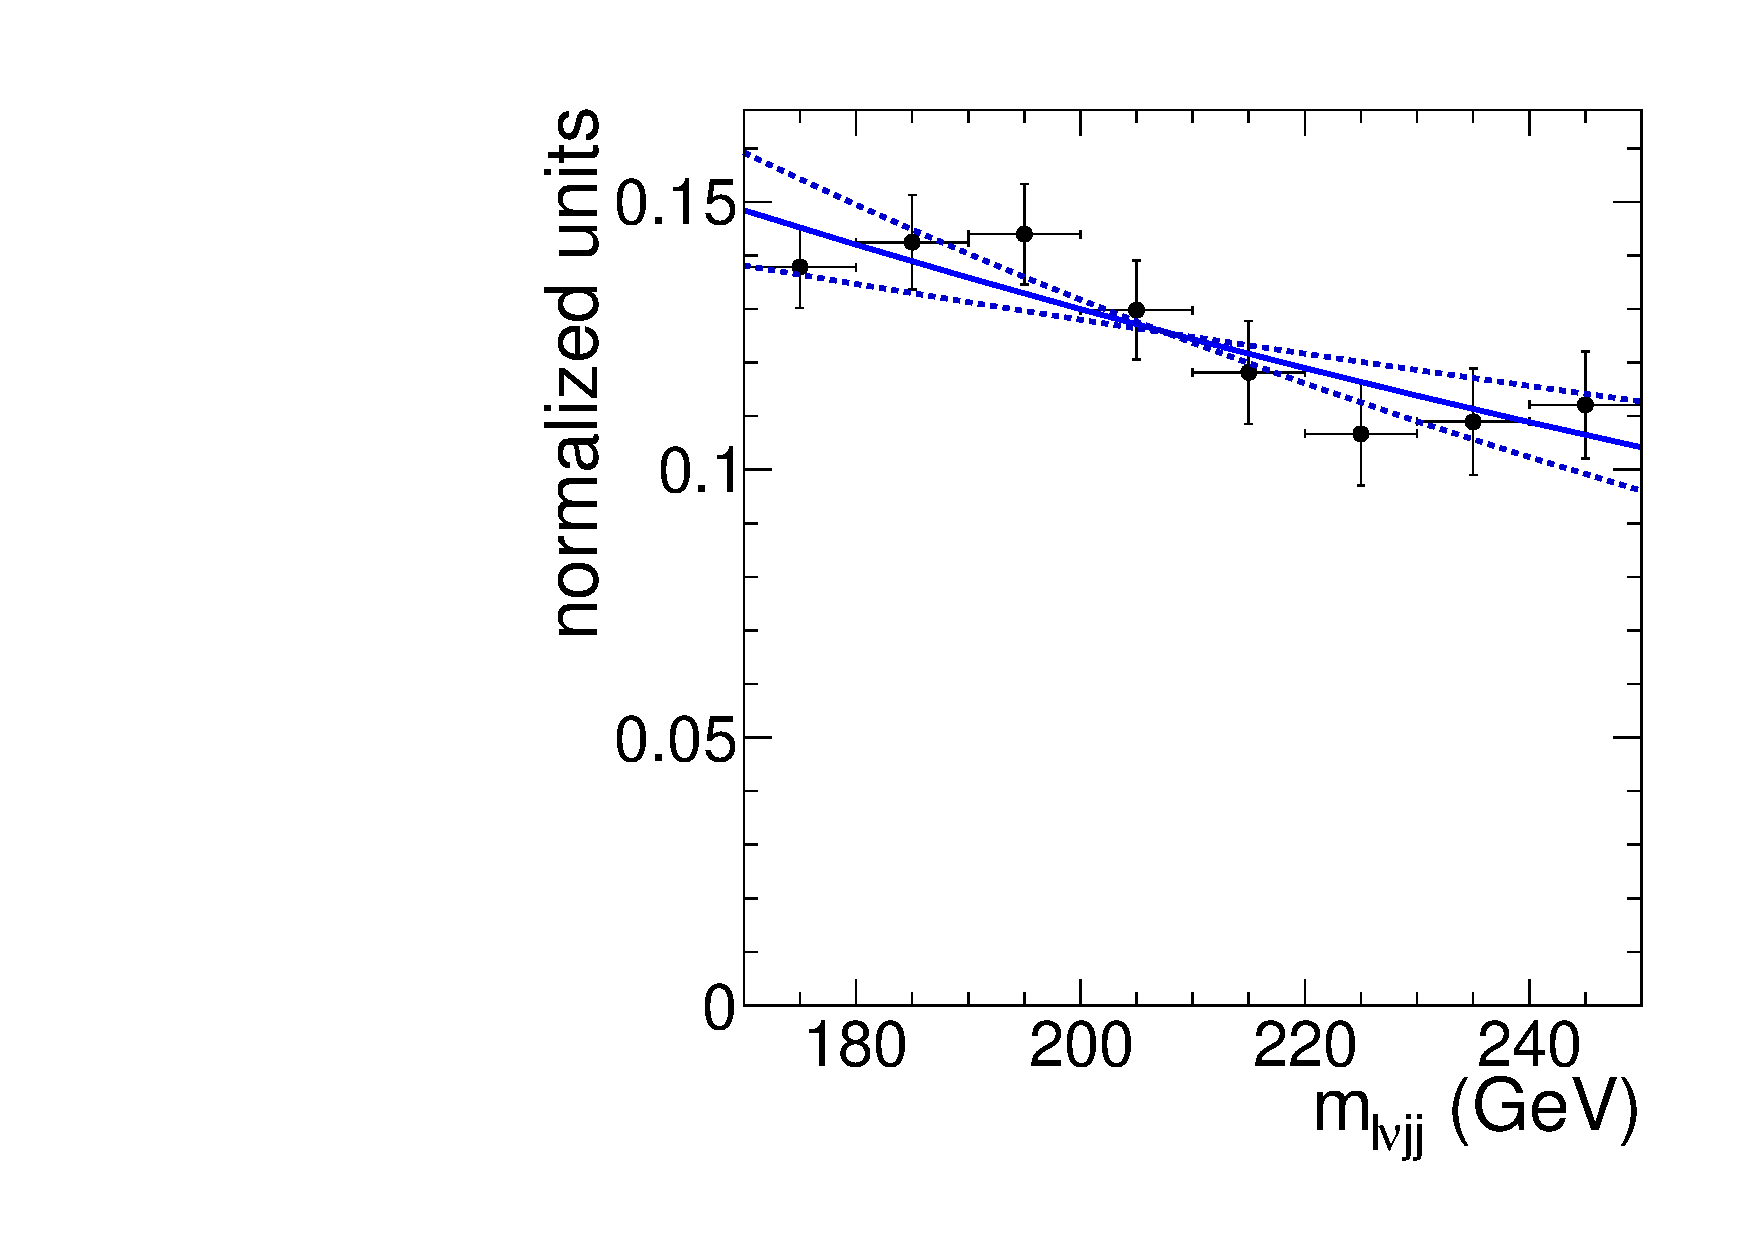
\includegraphics[width=0.49\textwidth]{plots/2012_WJetsShape/H180_Mlvjj_Muon_3jets_WpJShape.pdf}
  \caption{\label{fig:Wjets_dd_180}
  The distribution of the extrapolated background in the signal region
  is reported for the Higgs mass hypothesis of 180 GeV.
  On the top the 2 jets case, on the bottom the 3 jets case.
  Electrons are on the left, muons on the right.
  The points represent the extrapolated points, 
  while the red line shows the fitting function and the blue shaded band 
  the error from the fit.
    } 
\end{figure}
%
\begin{figure}[!t]
  \centering
    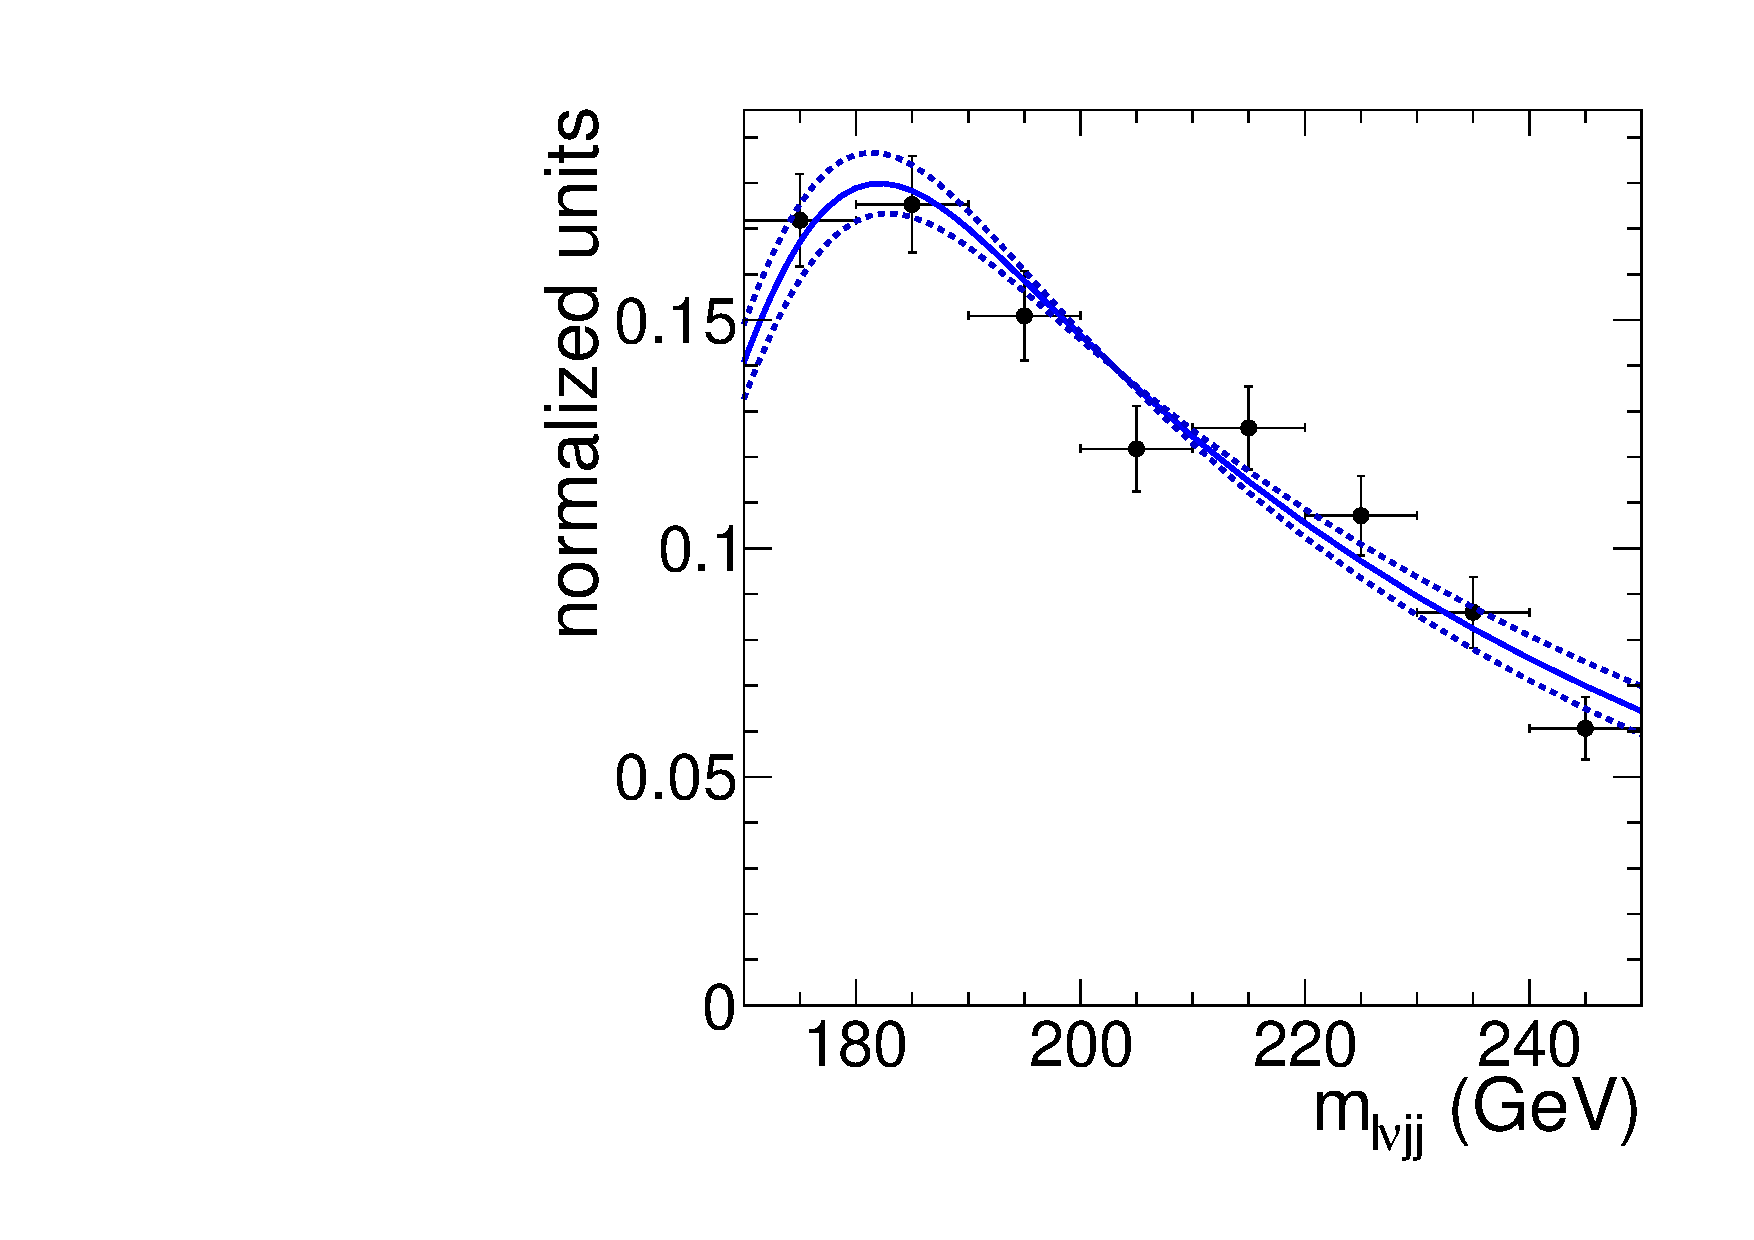
\includegraphics[width=0.49\textwidth]{plots/2012_WJetsShape/H190_Mlvjj_Electron_2jets_WpJShape.pdf}
    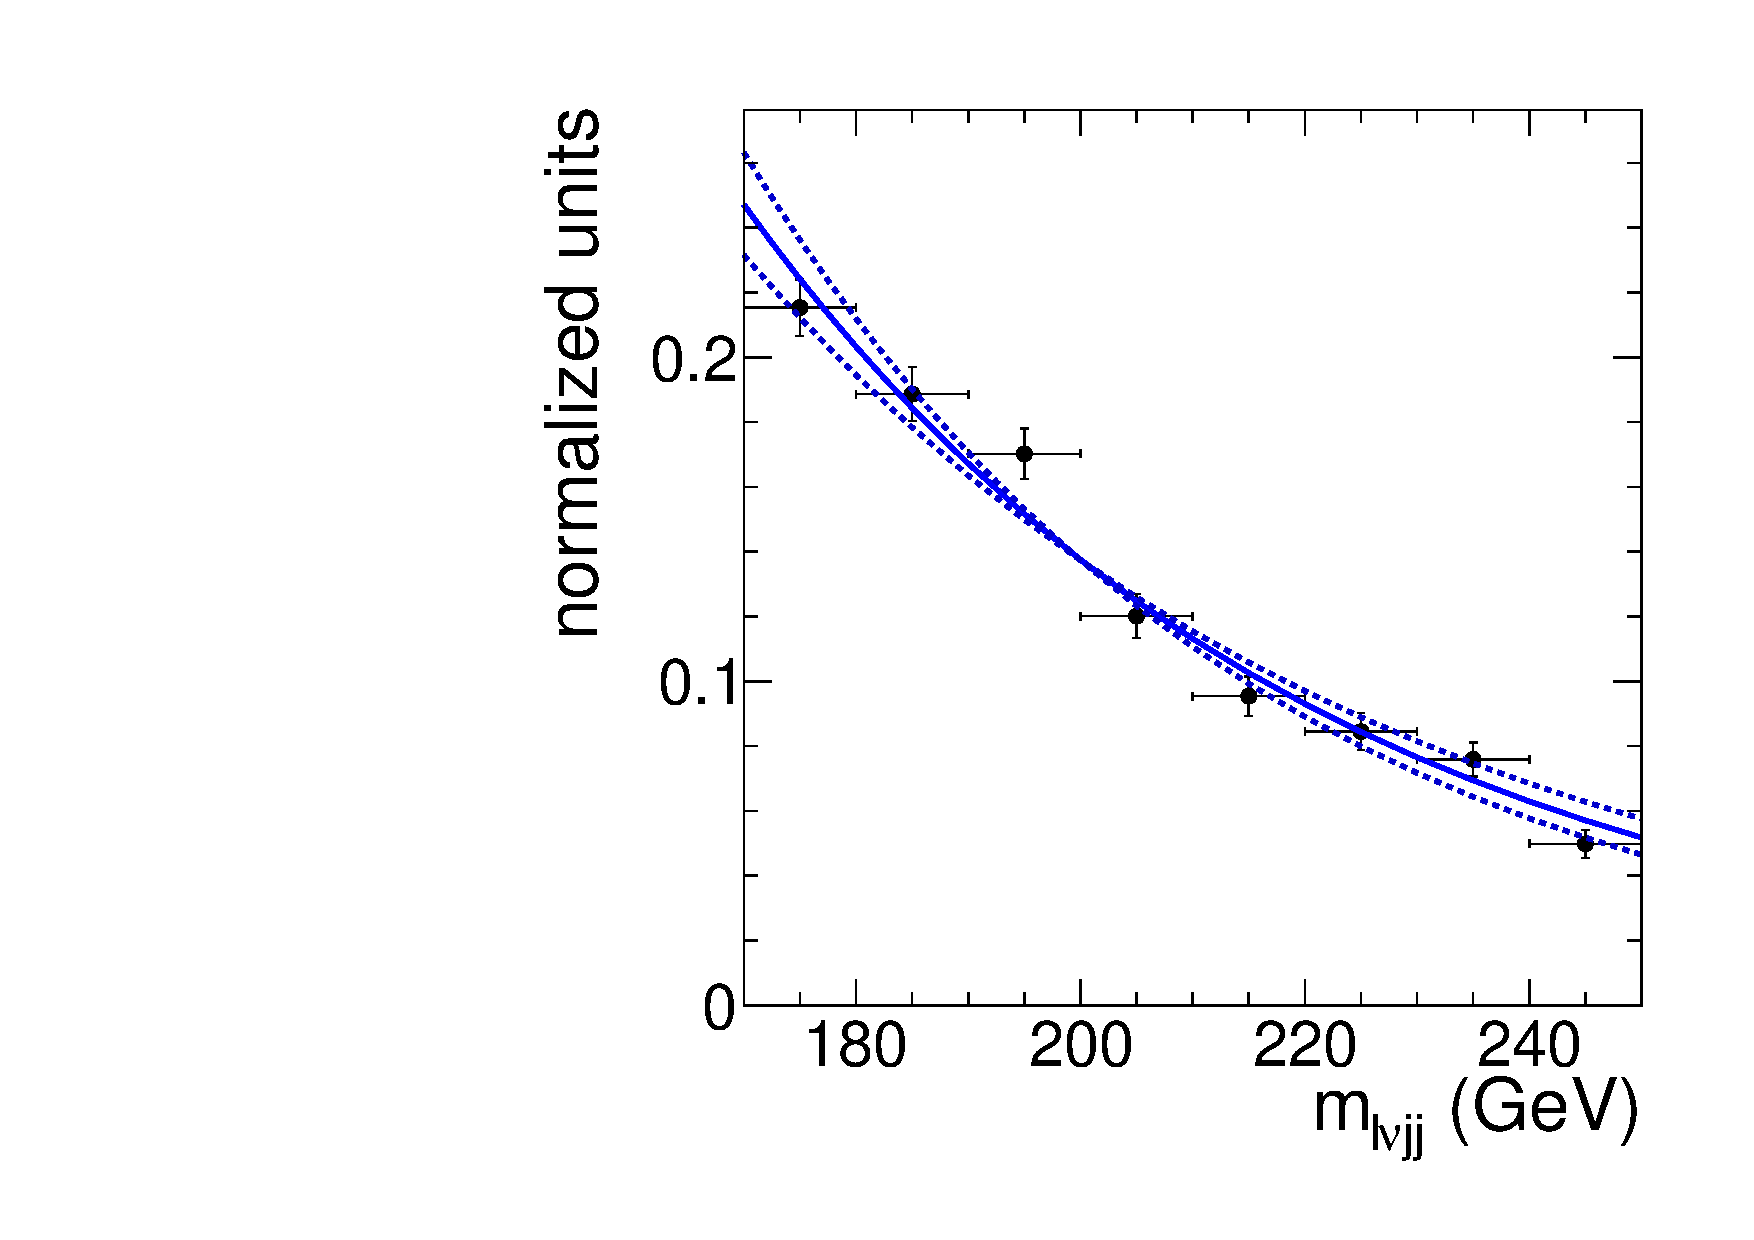
\includegraphics[width=0.49\textwidth]{plots/2012_WJetsShape/H190_Mlvjj_Muon_2jets_WpJShape.pdf}
    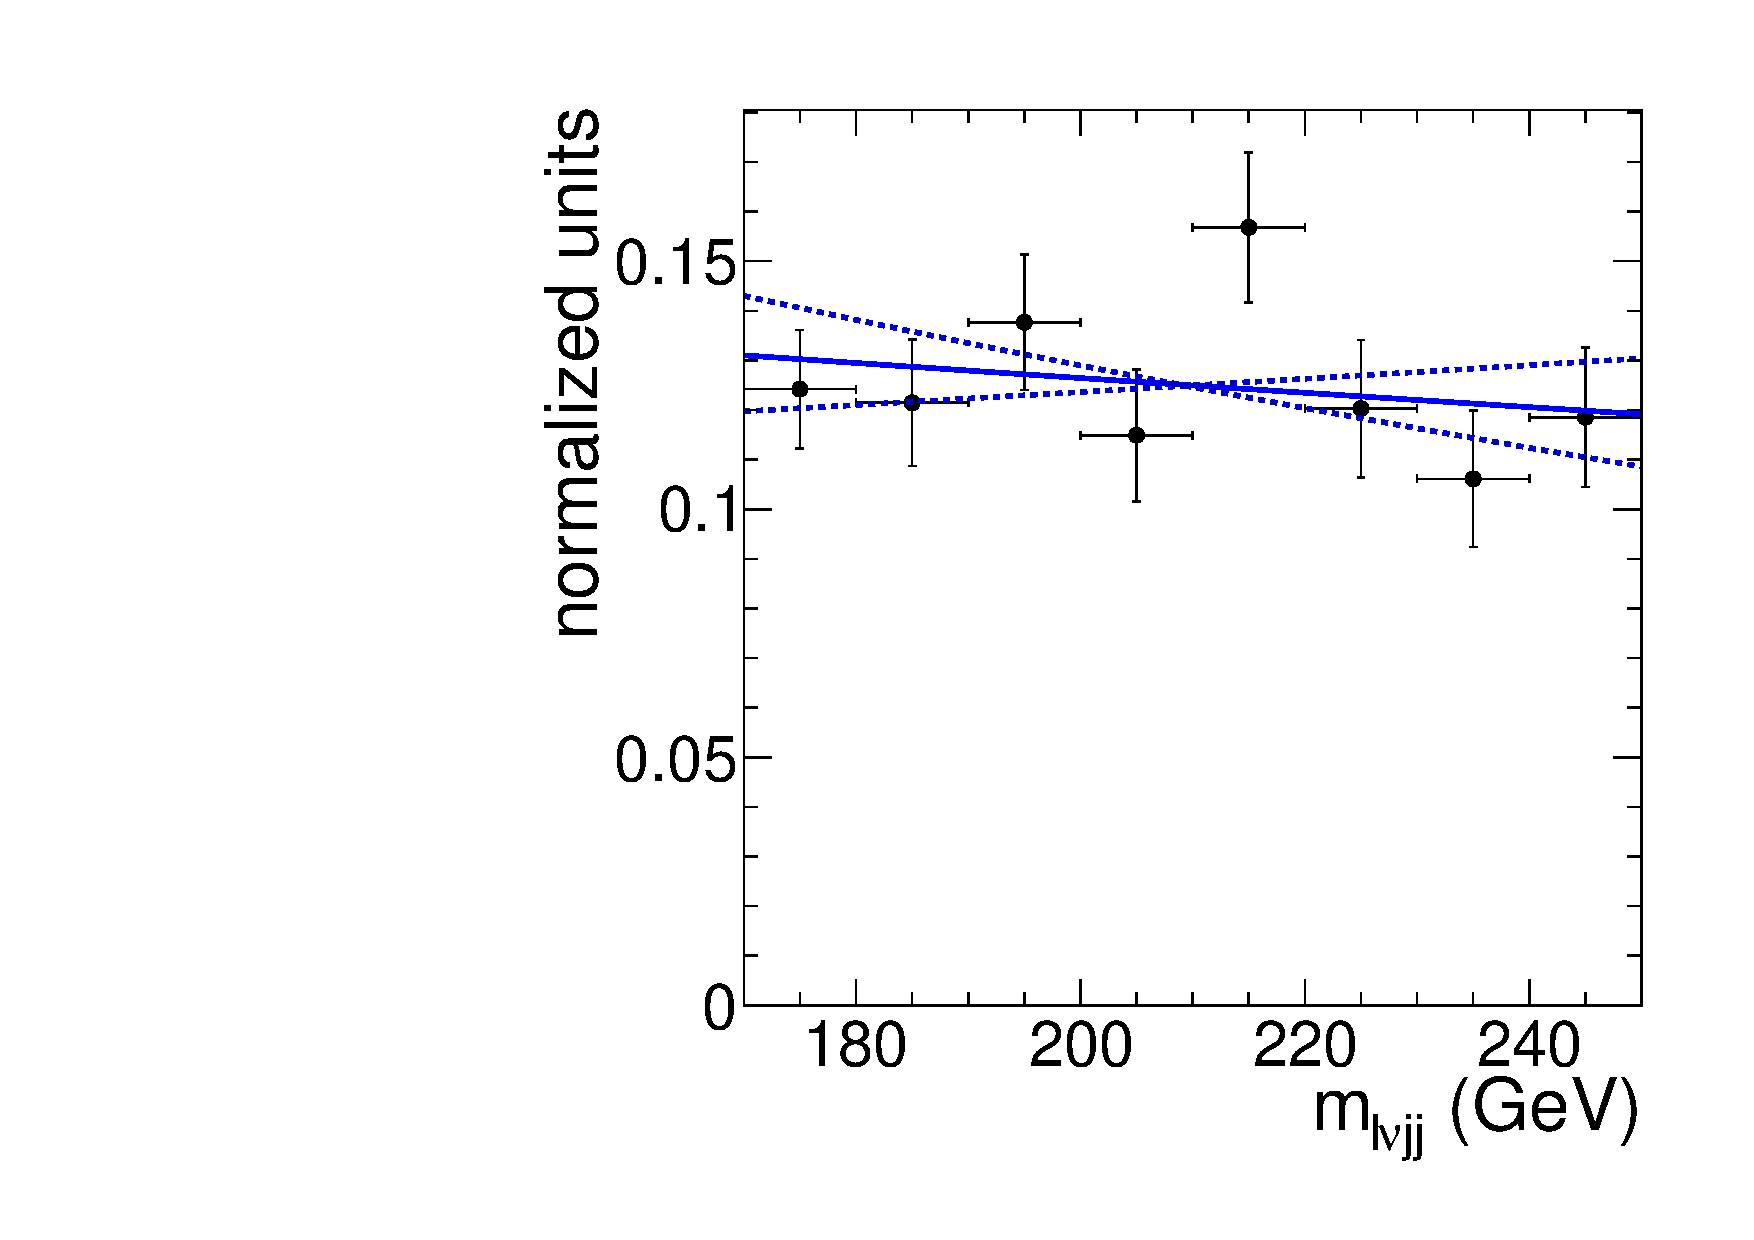
\includegraphics[width=0.49\textwidth]{plots/2012_WJetsShape/H190_Mlvjj_Electron_3jets_WpJShape.pdf}
    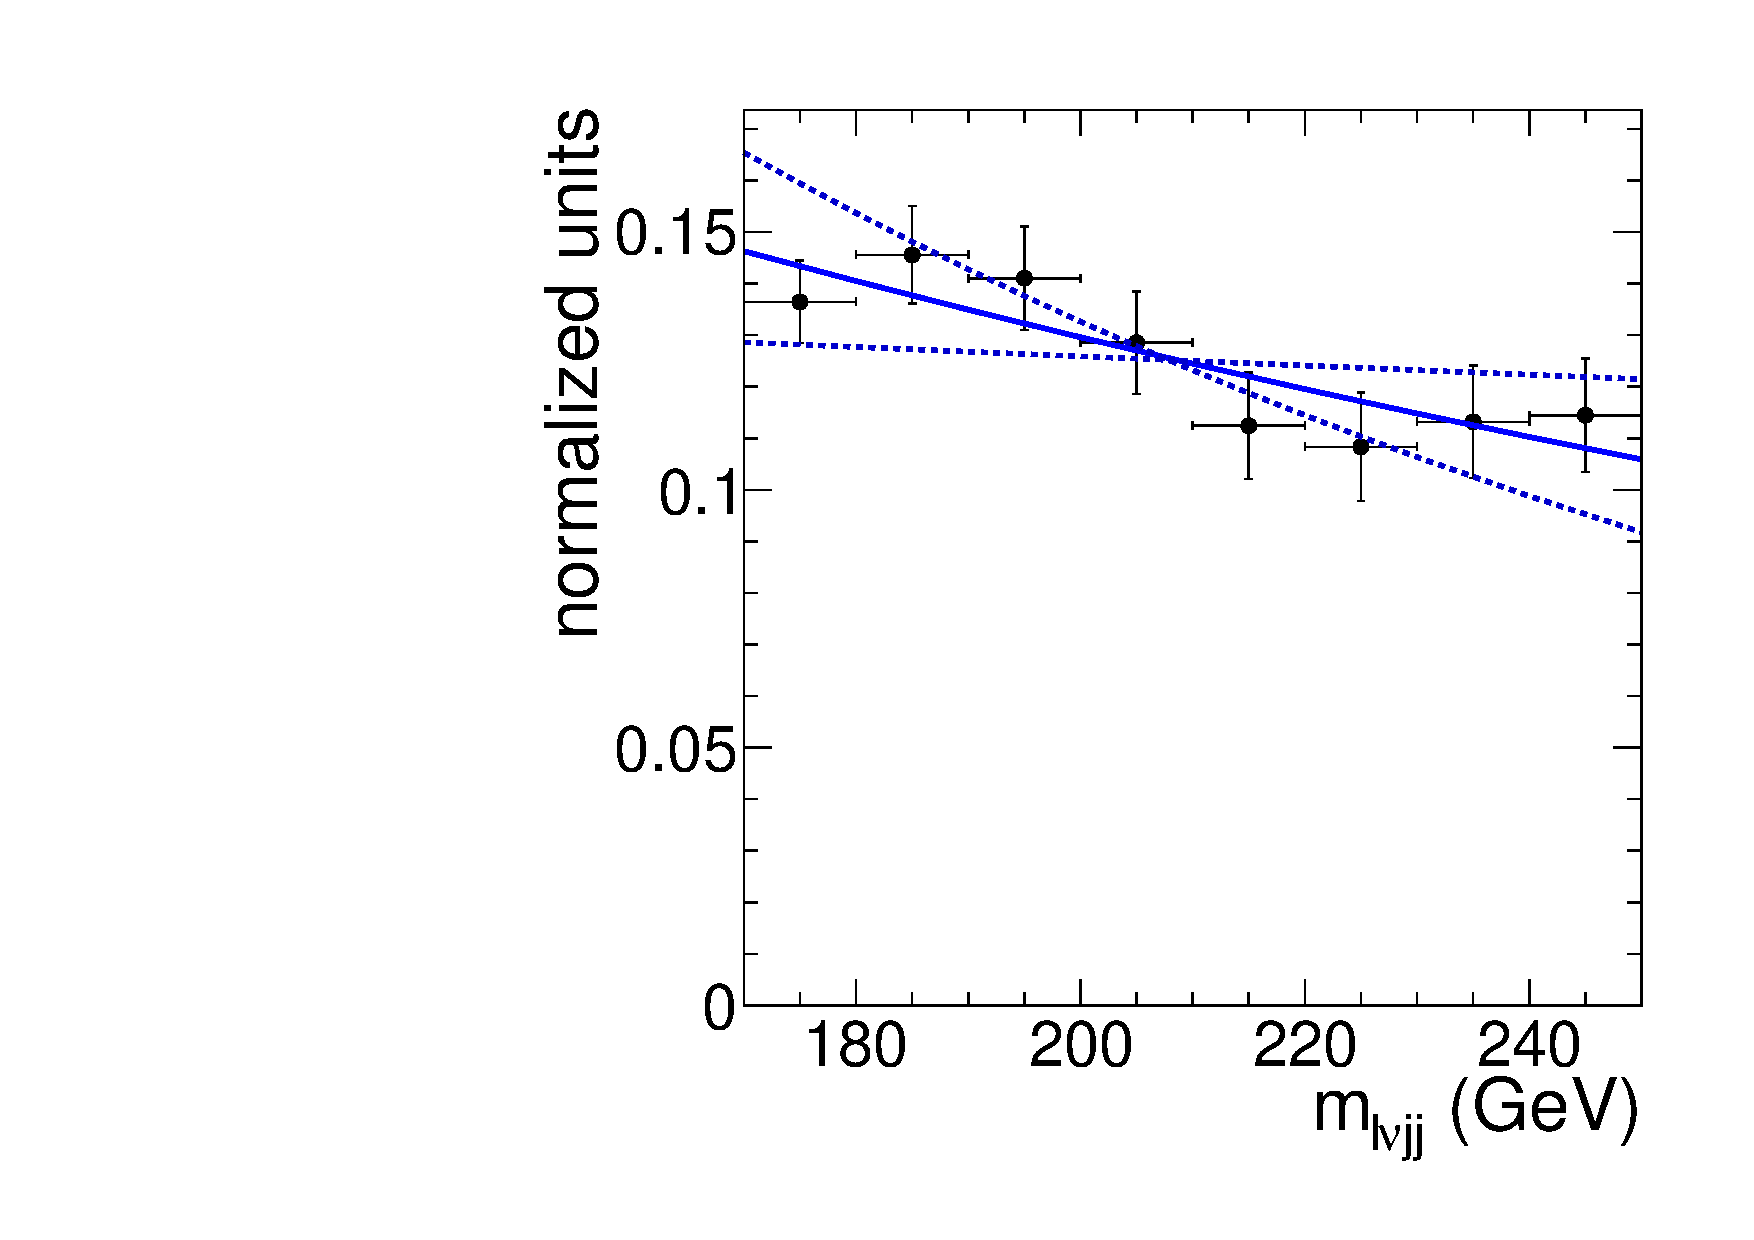
\includegraphics[width=0.49\textwidth]{plots/2012_WJetsShape/H190_Mlvjj_Muon_3jets_WpJShape.pdf}
  \caption{\label{fig:Wjets_dd_190}
  The distribution of the extrapolated background in the signal region
  is reported for the Higgs mass hypothesis of 190 GeV.
  On the top the 2 jets case, on the bottom the 3 jets case.
  Electrons are on the left, muons on the right.
  The points represent the extrapolated points, 
  while the red line shows the fitting function and the blue shaded band 
  the error from the fit.
    } 
\end{figure}
%
\begin{figure}[!t]
  \centering
    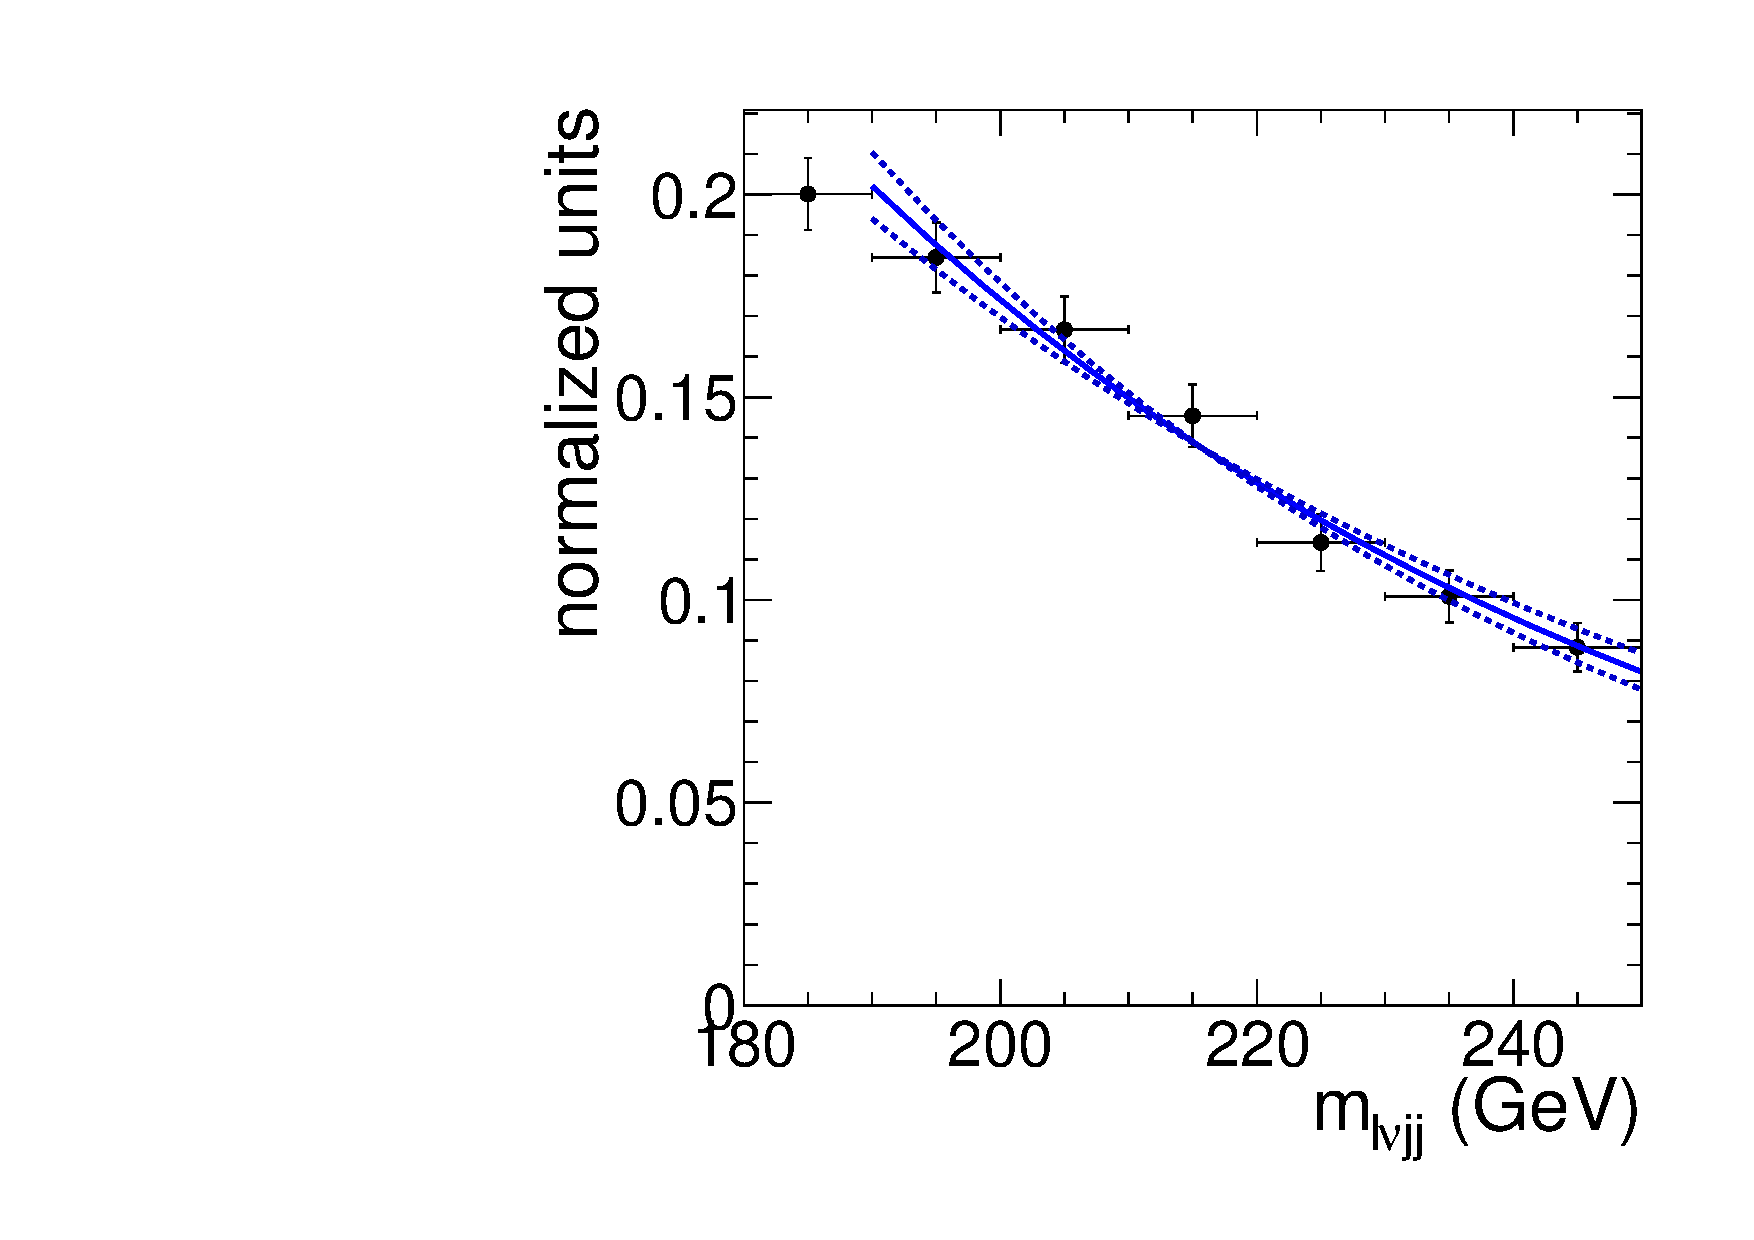
\includegraphics[width=0.49\textwidth]{plots/2012_WJetsShape/H200_Mlvjj_Electron_2jets_WpJShape.pdf}
    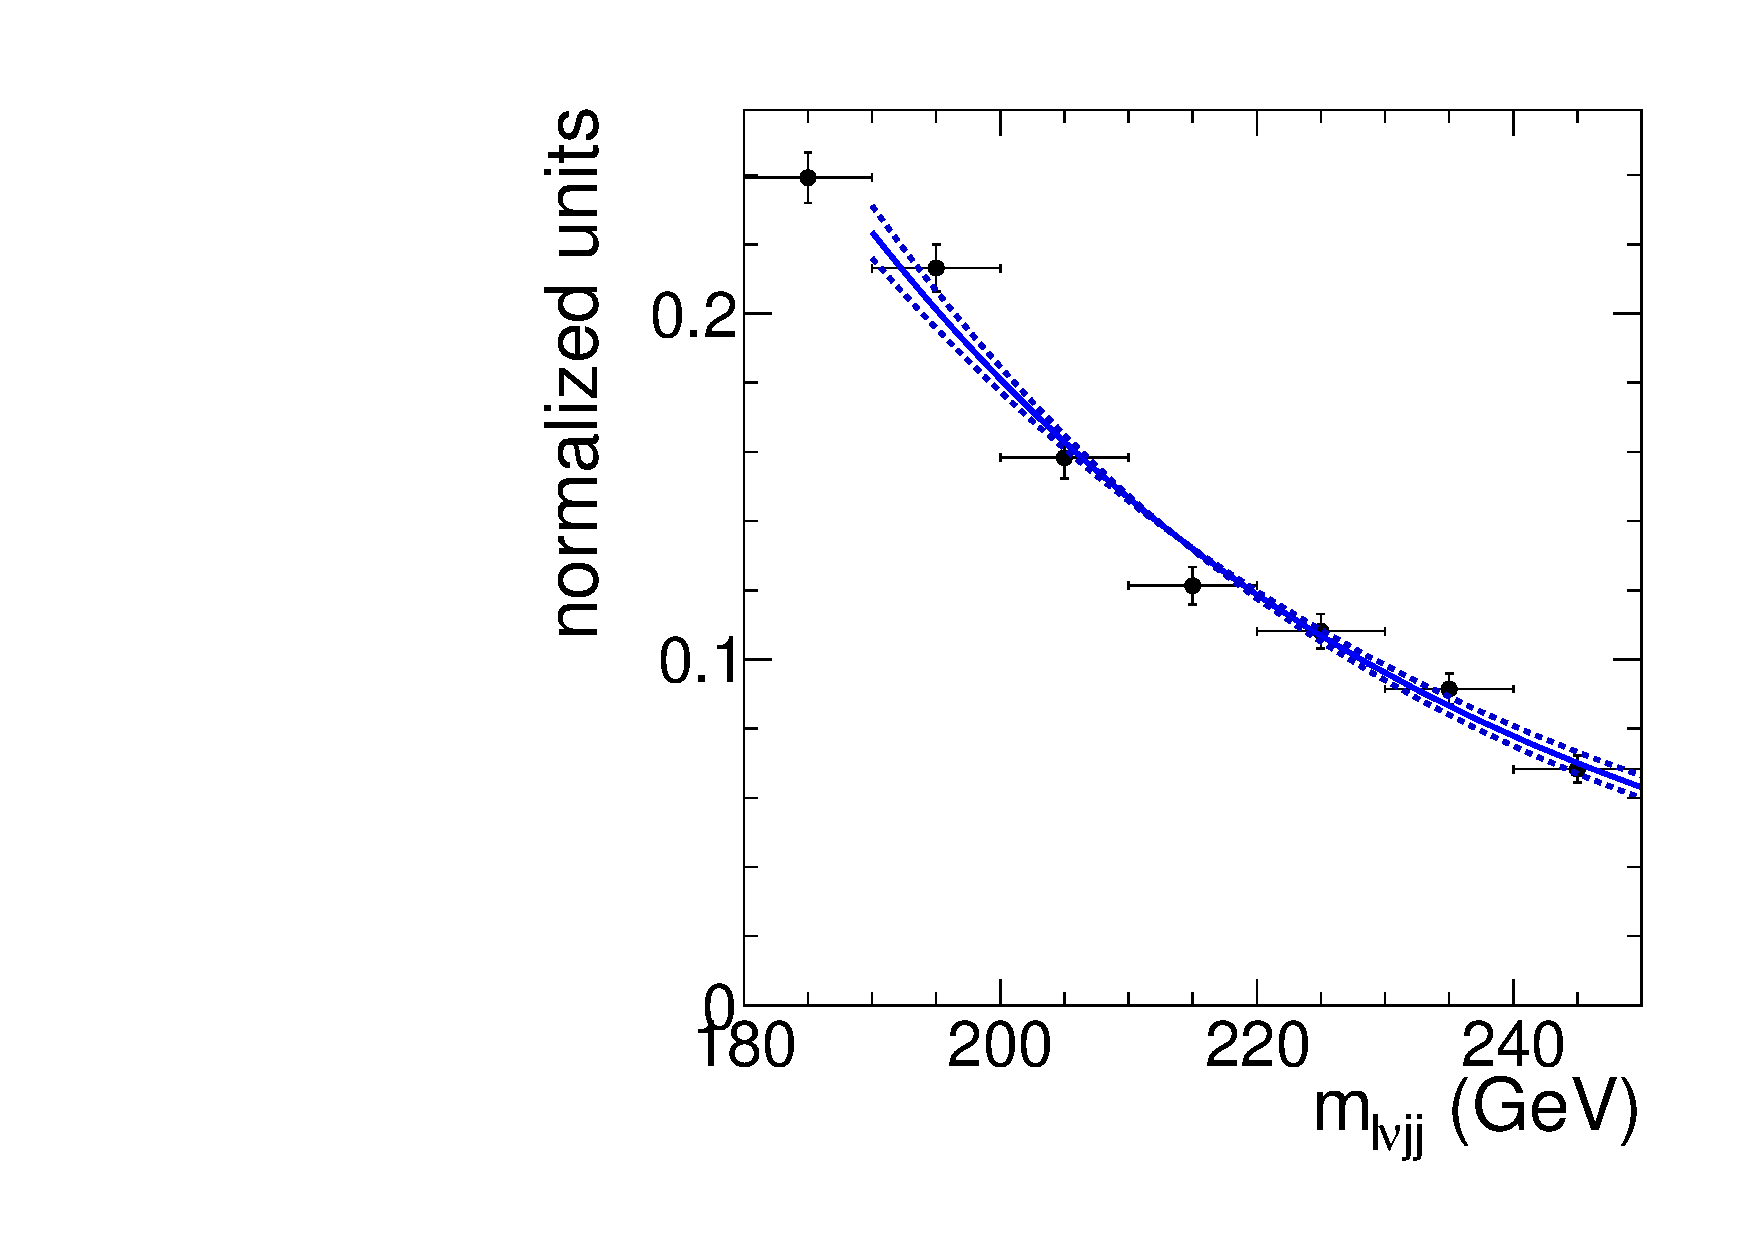
\includegraphics[width=0.49\textwidth]{plots/2012_WJetsShape/H200_Mlvjj_Muon_2jets_WpJShape.pdf}
    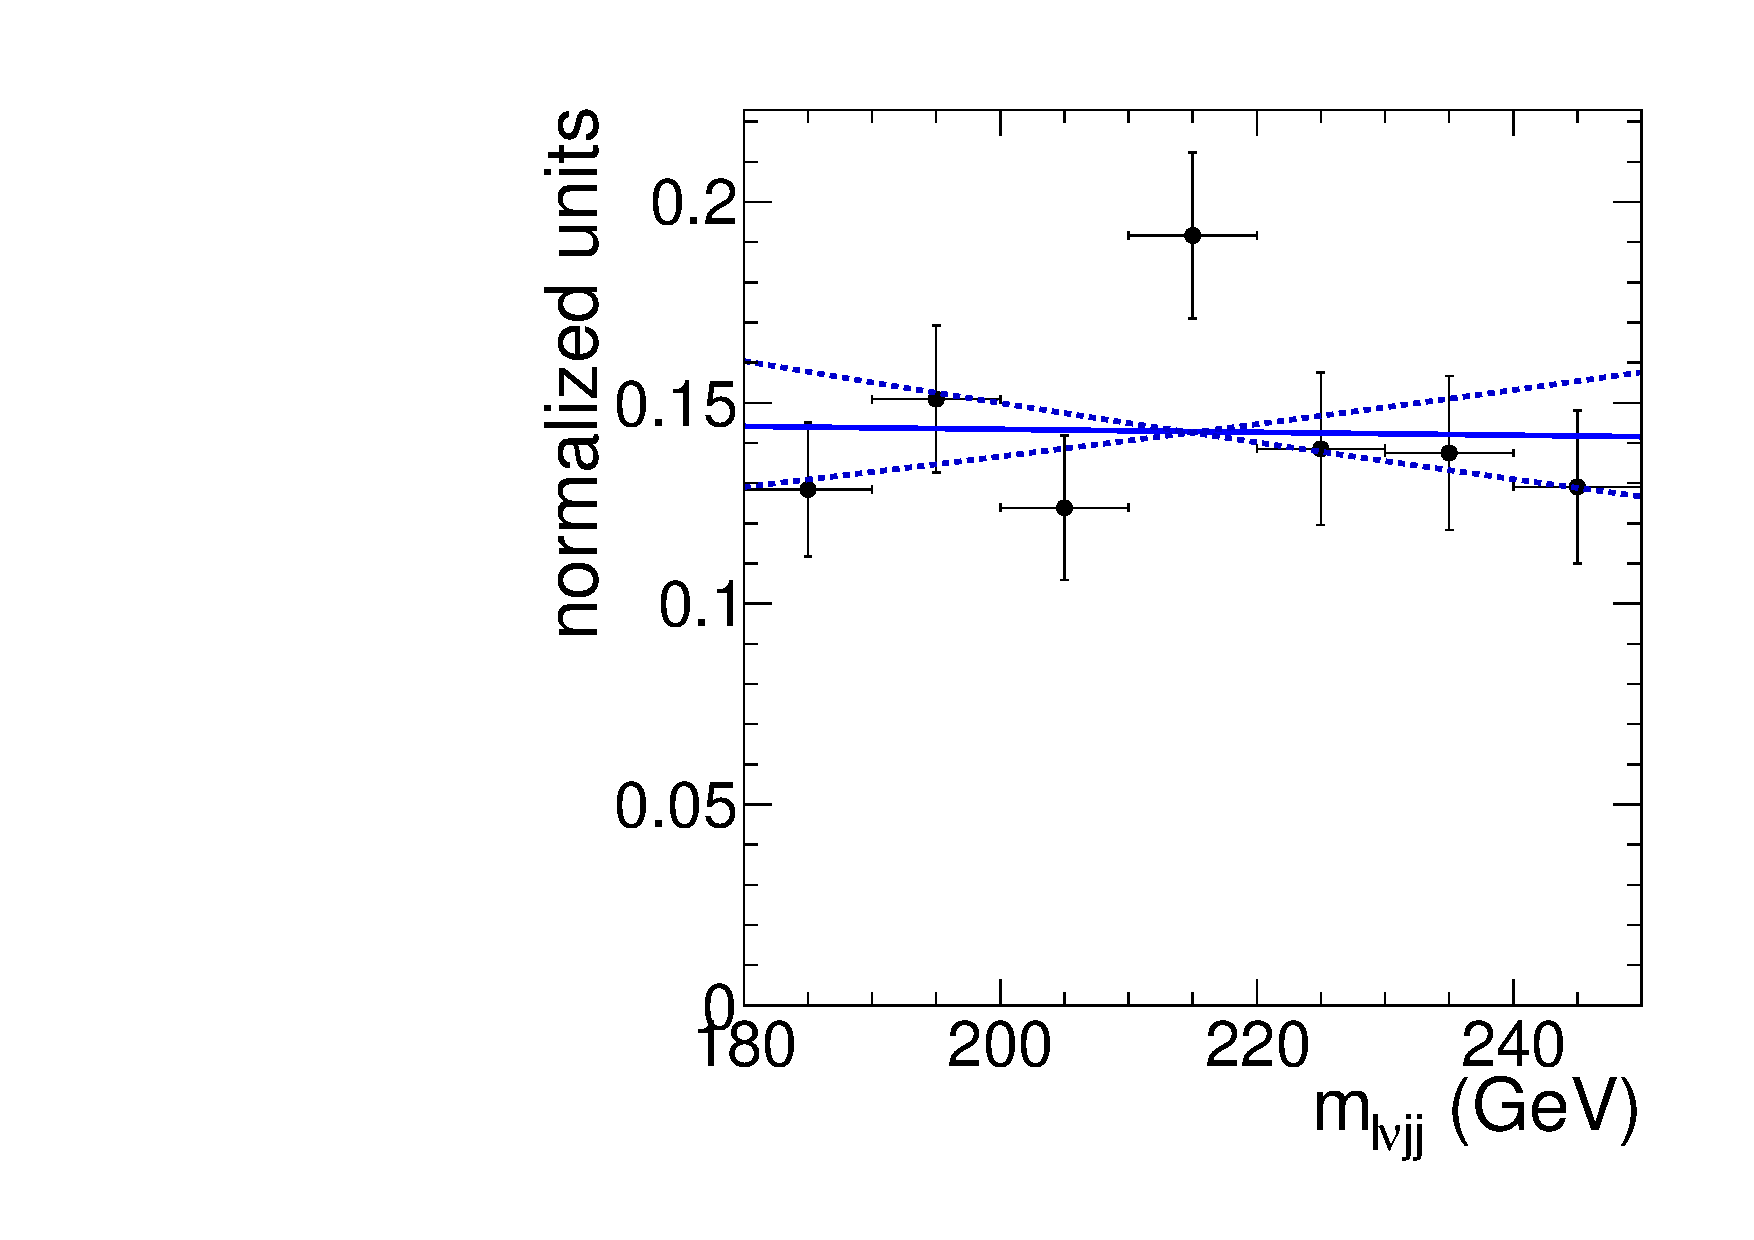
\includegraphics[width=0.49\textwidth]{plots/2012_WJetsShape/H200_Mlvjj_Electron_3jets_WpJShape.pdf}
    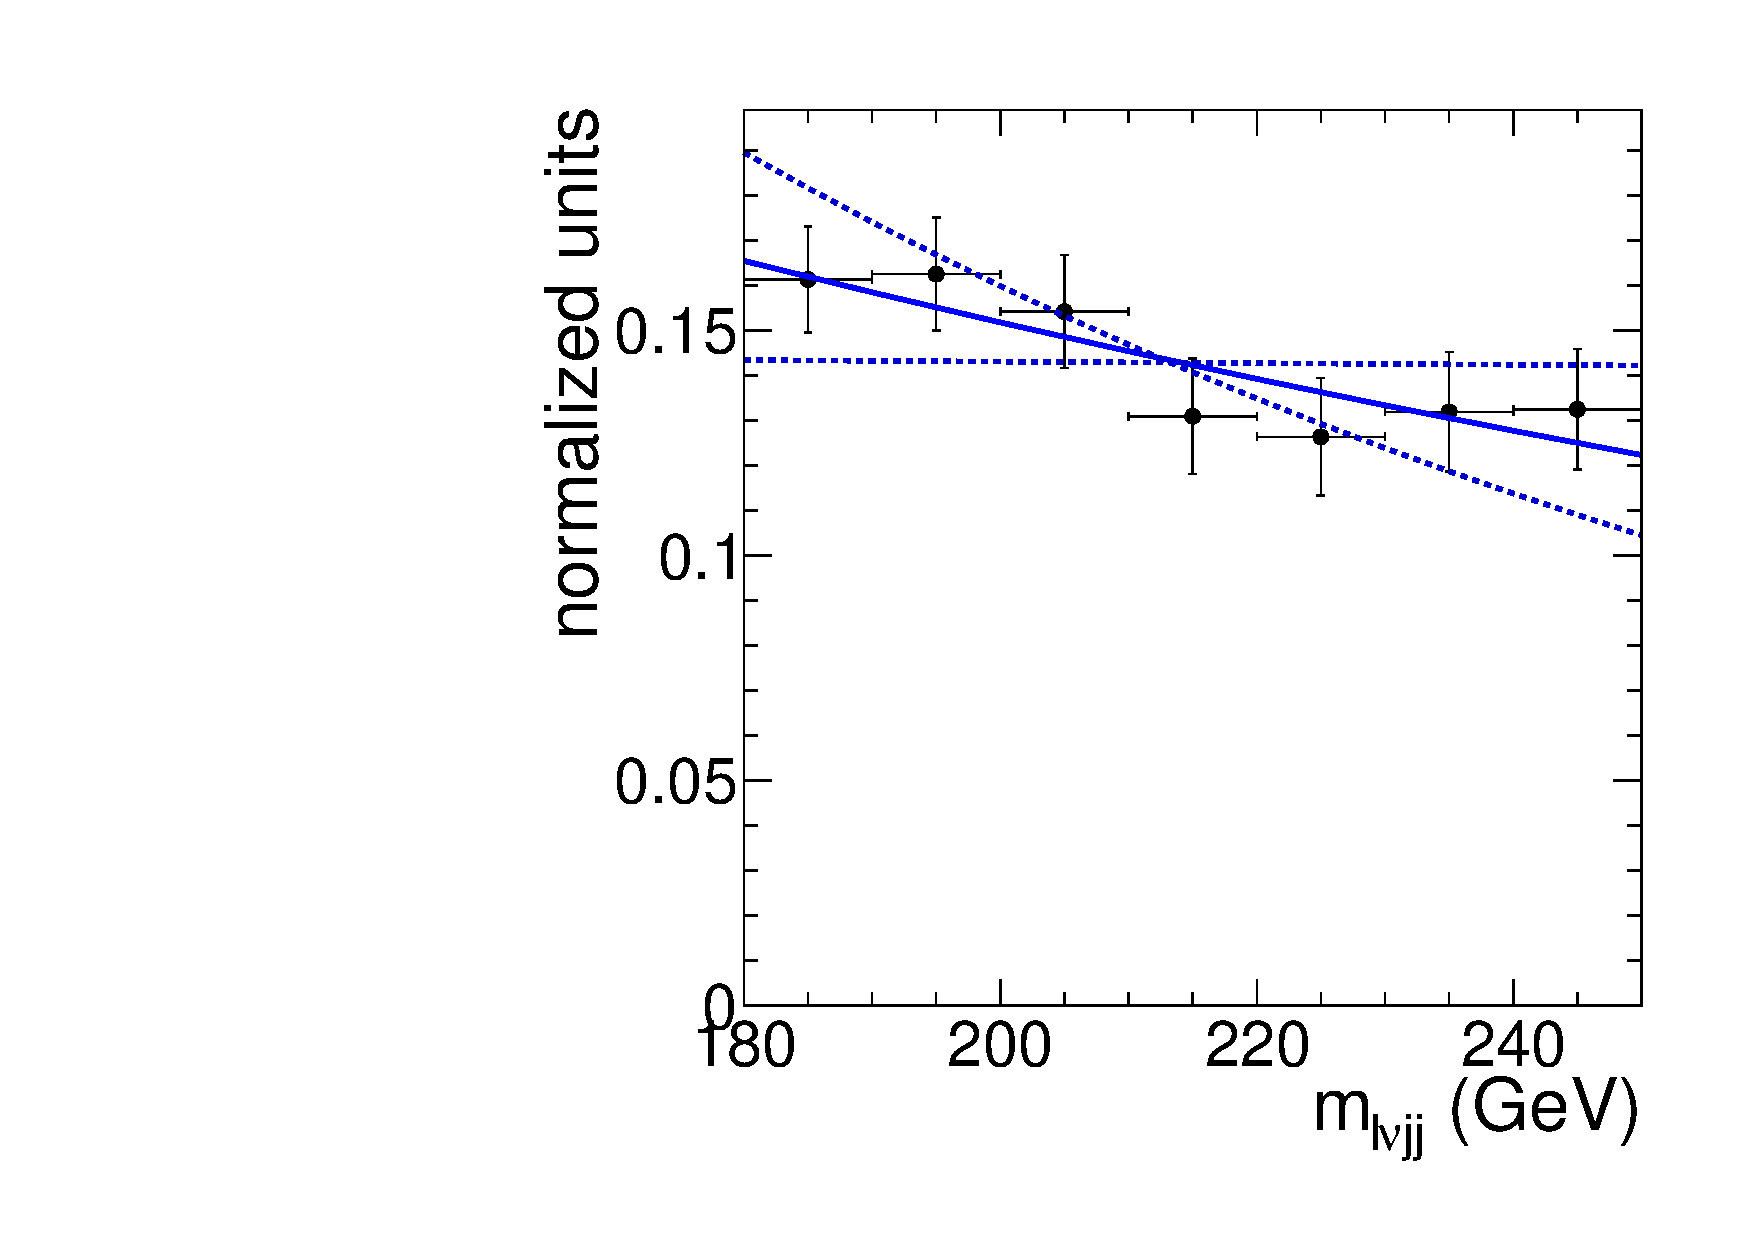
\includegraphics[width=0.49\textwidth]{plots/2012_WJetsShape/H200_Mlvjj_Muon_3jets_WpJShape.pdf}
  \caption{\label{fig:Wjets_dd_200}
  The distribution of the extrapolated background in the signal region
  is reported for the Higgs mass hypothesis of 200 GeV.
  On the top the 2 jets case, on the bottom the 3 jets case.
  Electrons are on the left, muons on the right.
  The points represent the extrapolated points, 
  while the red line shows the fitting function and the blue shaded band 
  the error from the fit.
    } 
\end{figure}
%
\begin{figure}[!t]
  \centering
    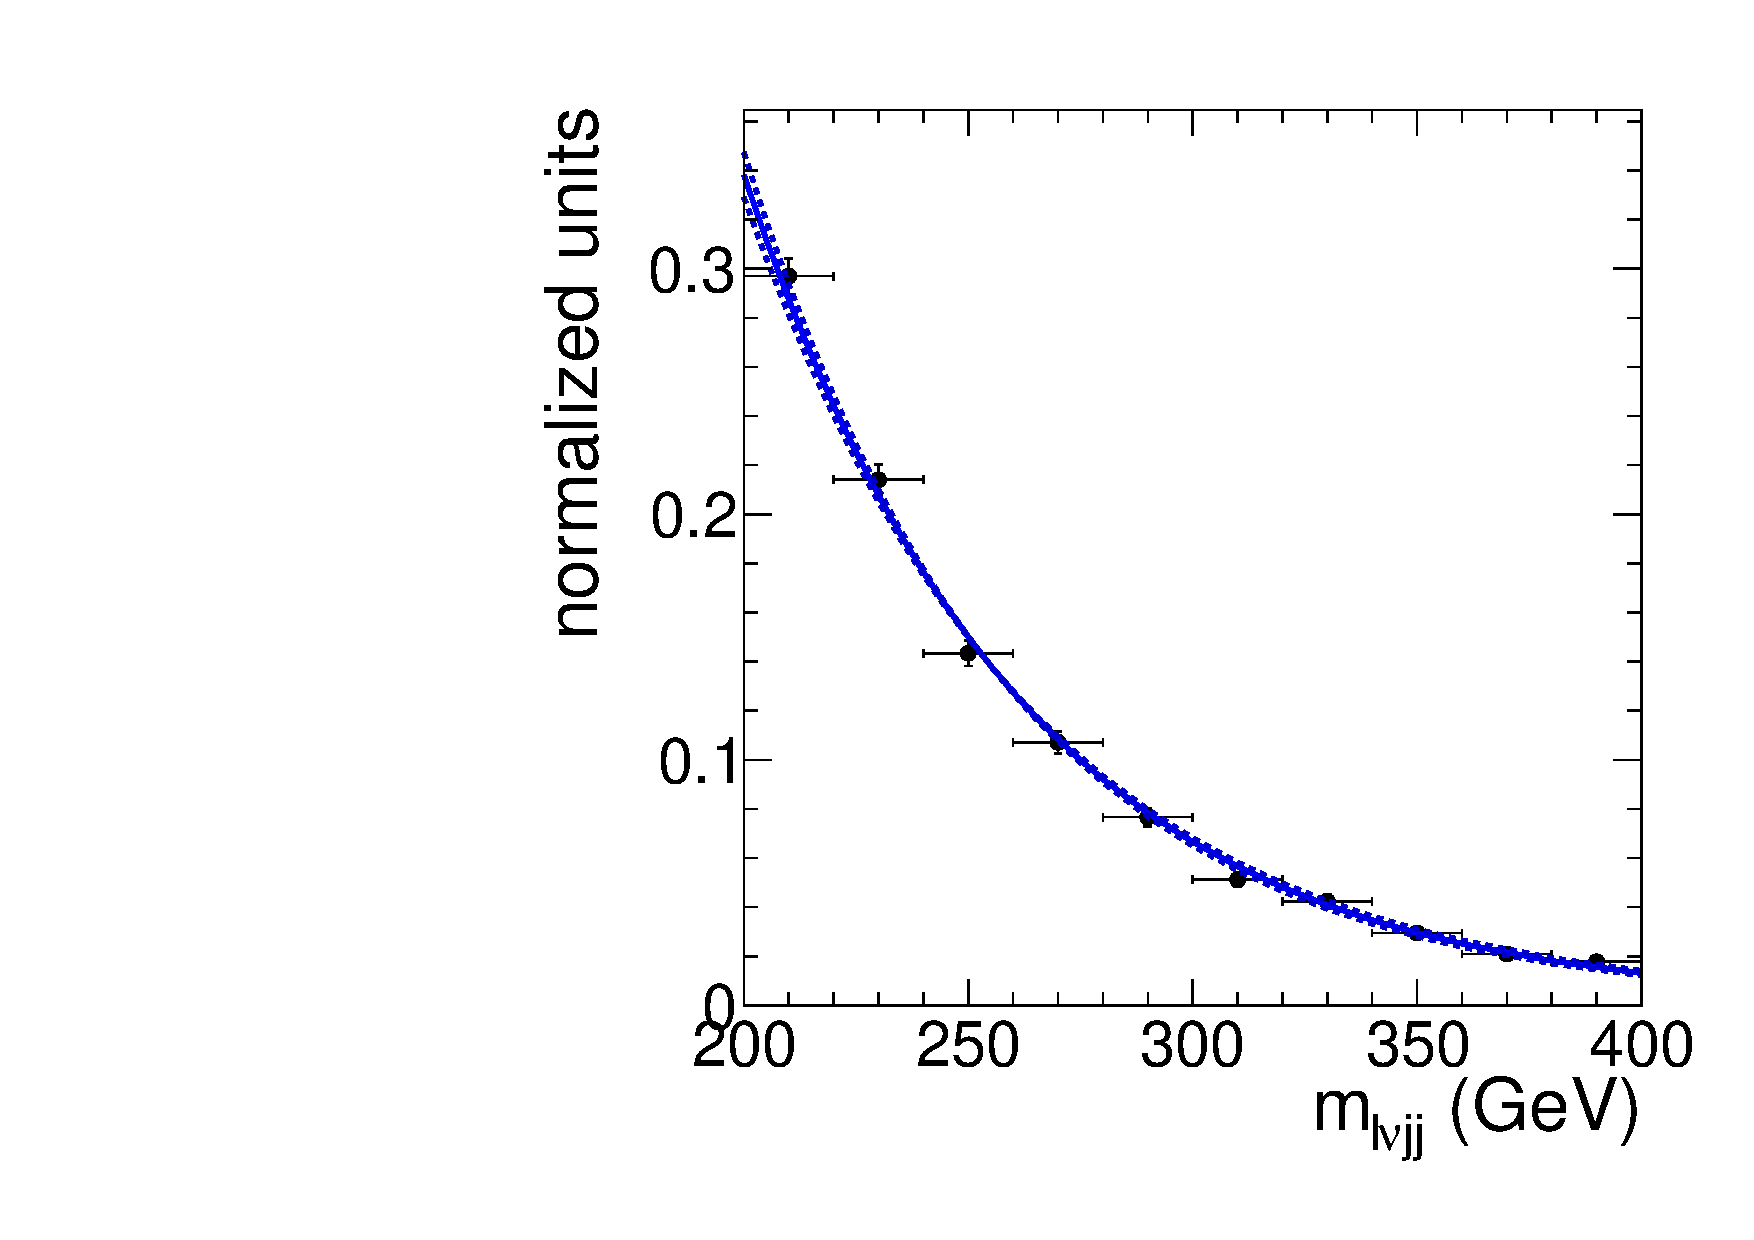
\includegraphics[width=0.49\textwidth]{plots/2012_WJetsShape/H250_Mlvjj_Electron_2jets_WpJShape.pdf}
    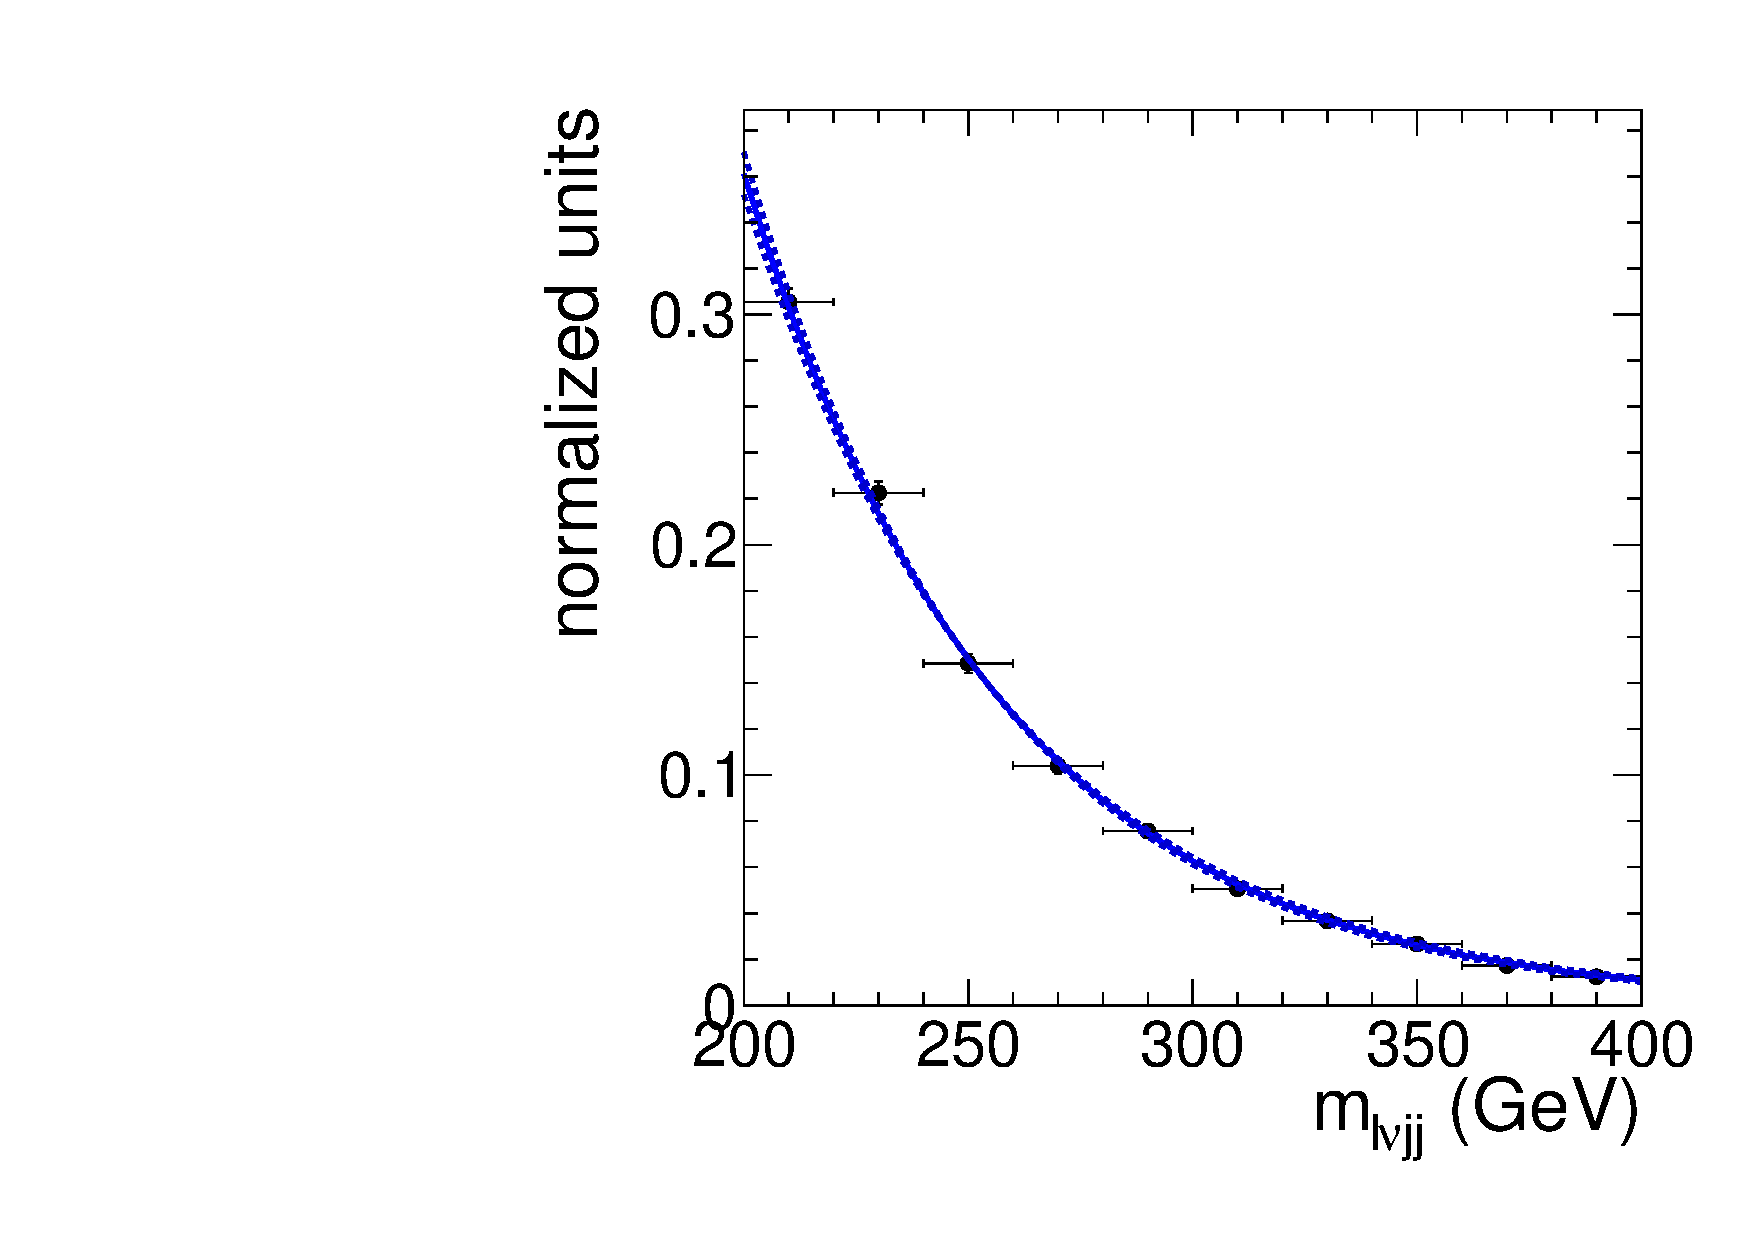
\includegraphics[width=0.49\textwidth]{plots/2012_WJetsShape/H250_Mlvjj_Muon_2jets_WpJShape.pdf}
    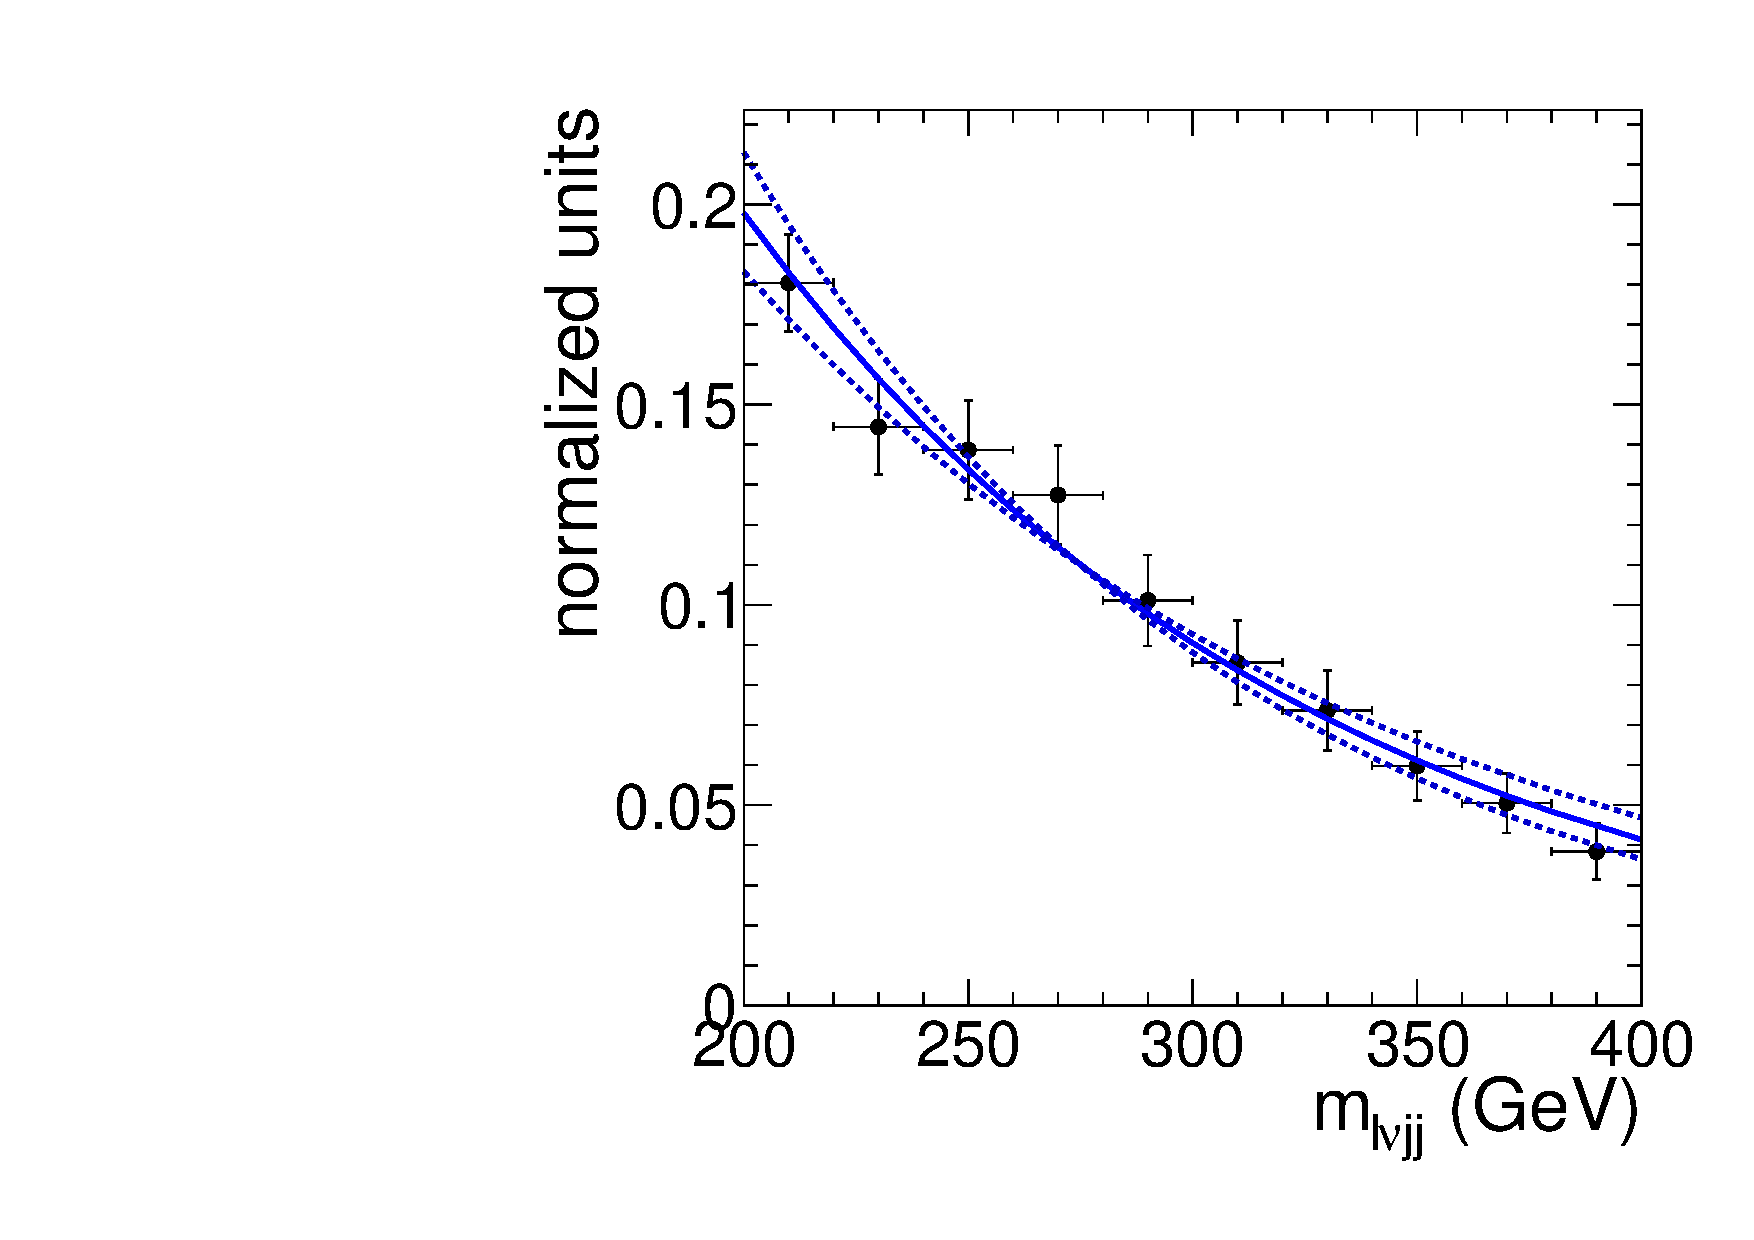
\includegraphics[width=0.49\textwidth]{plots/2012_WJetsShape/H250_Mlvjj_Electron_3jets_WpJShape.pdf}
    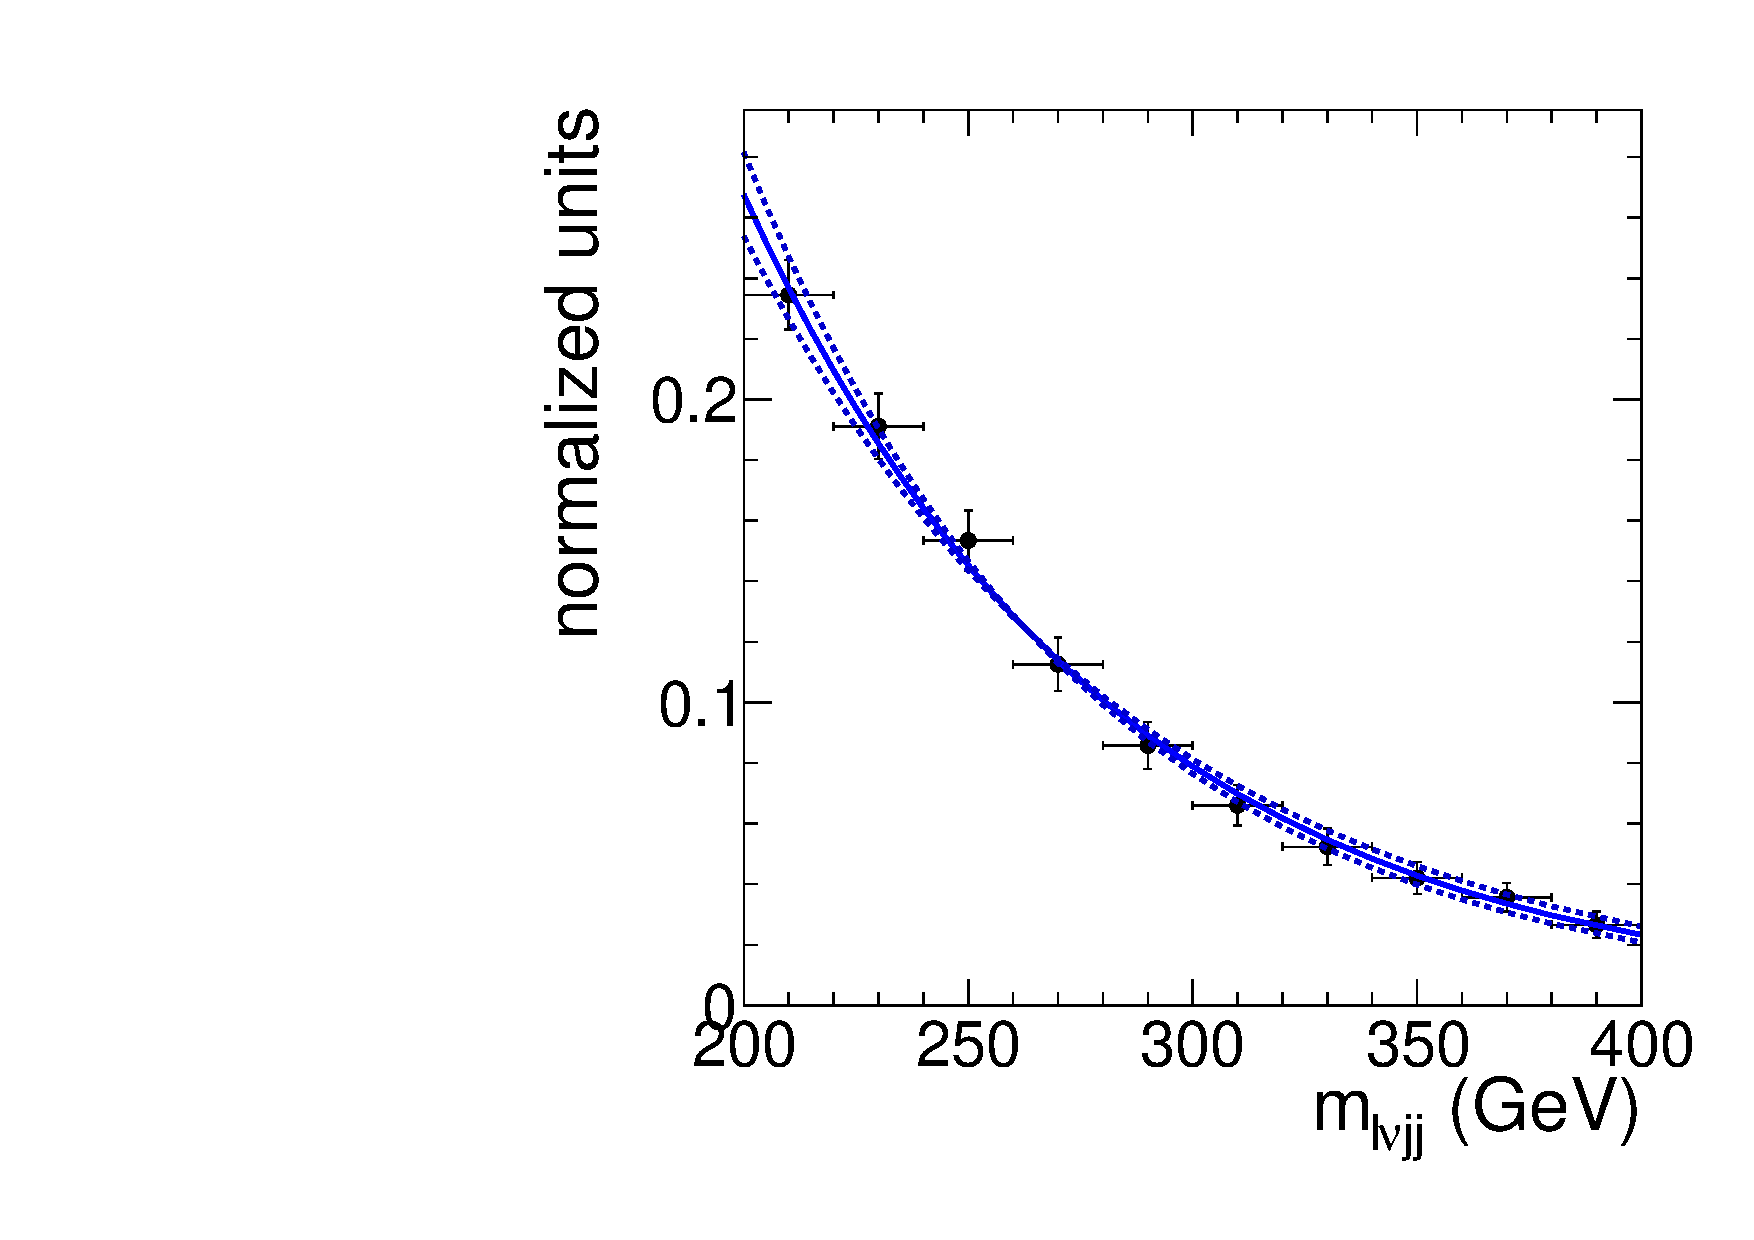
\includegraphics[width=0.49\textwidth]{plots/2012_WJetsShape/H250_Mlvjj_Muon_3jets_WpJShape.pdf}
  \caption{\label{fig:Wjets_dd_250}
  The distribution of the extrapolated background in the signal region
  is reported for the Higgs mass hypothesis of 250 GeV.
  On the top the 2 jets case, on the bottom the 3 jets case.
  Electrons are on the left, muons on the right.
  The points represent the extrapolated points, 
  while the red line shows the fitting function and the blue shaded band 
  the error from the fit.
    } 
\end{figure}
%
\begin{figure}[!t]
  \centering
    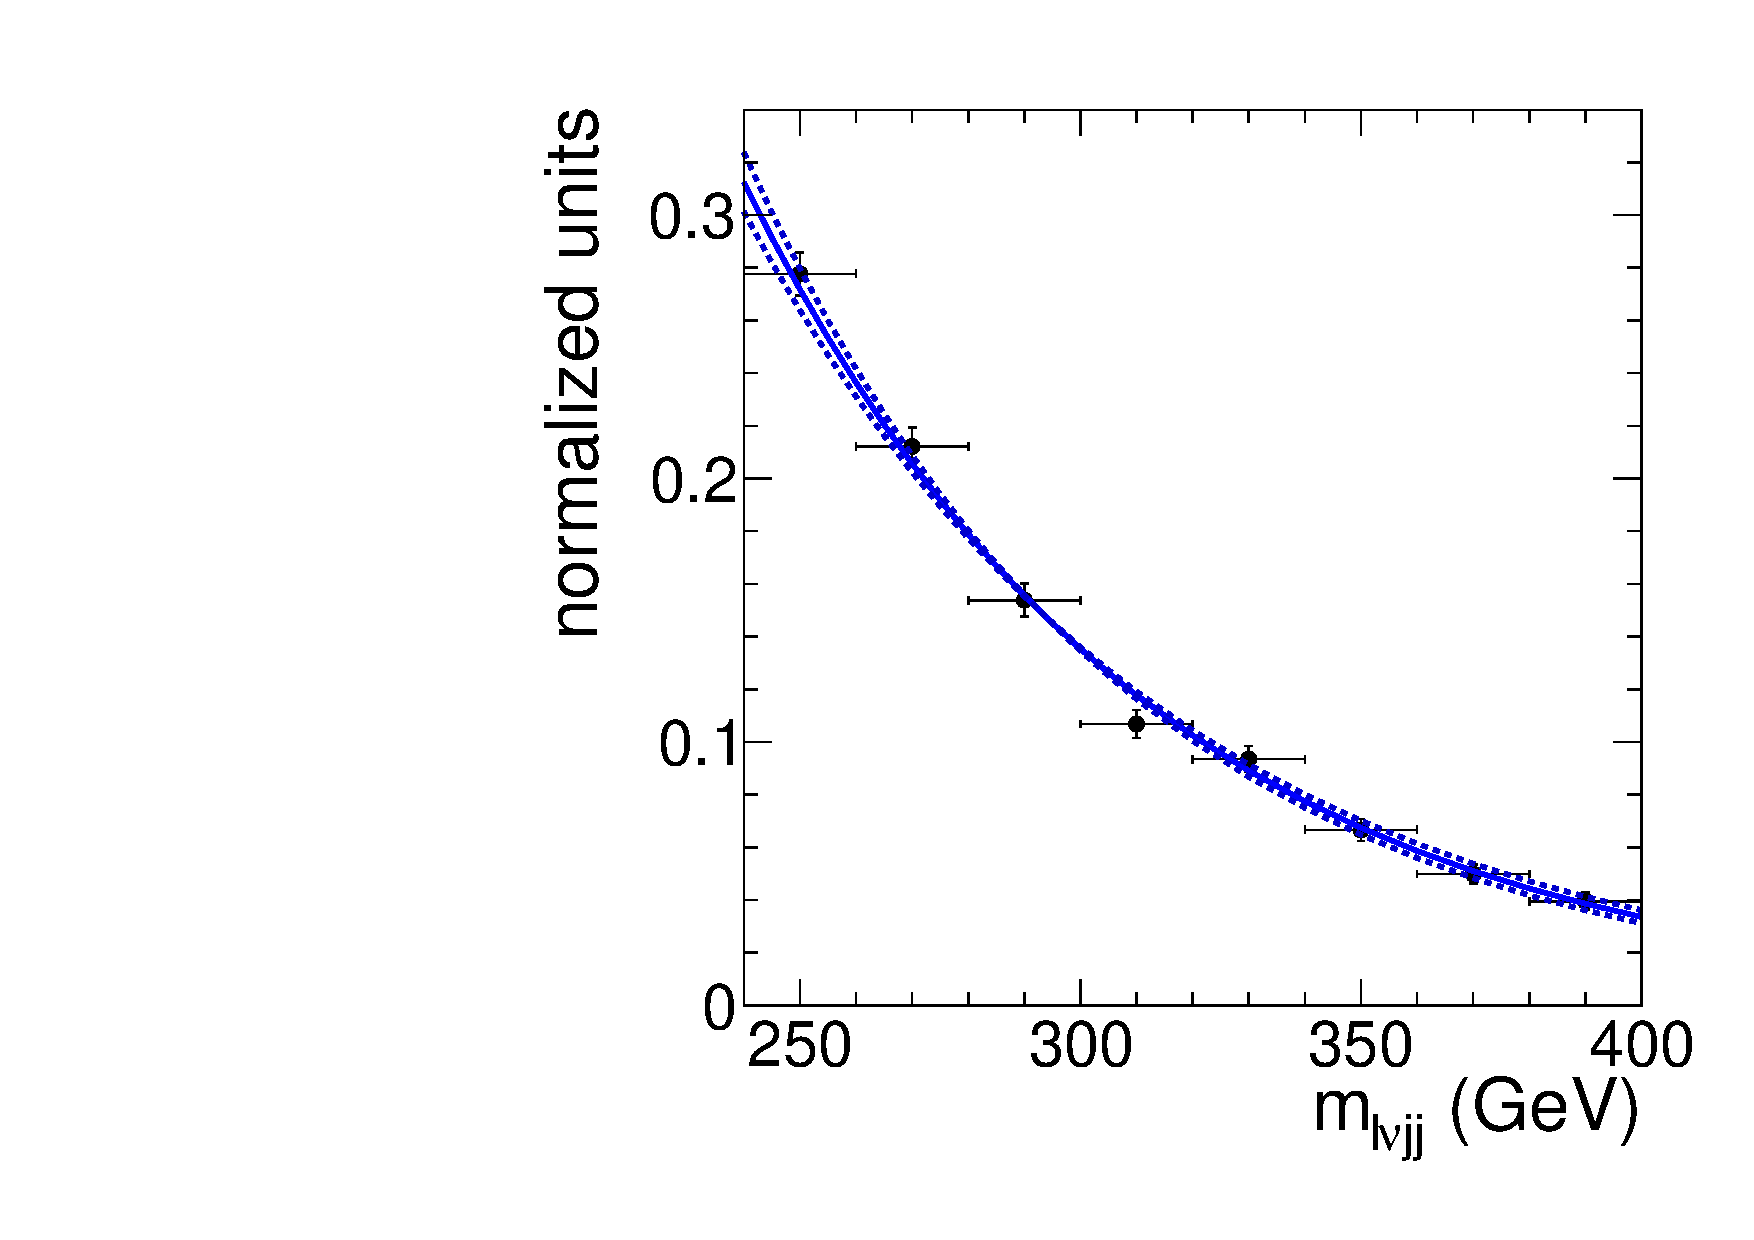
\includegraphics[width=0.49\textwidth]{plots/2012_WJetsShape/H300_Mlvjj_Electron_2jets_WpJShape.pdf}
    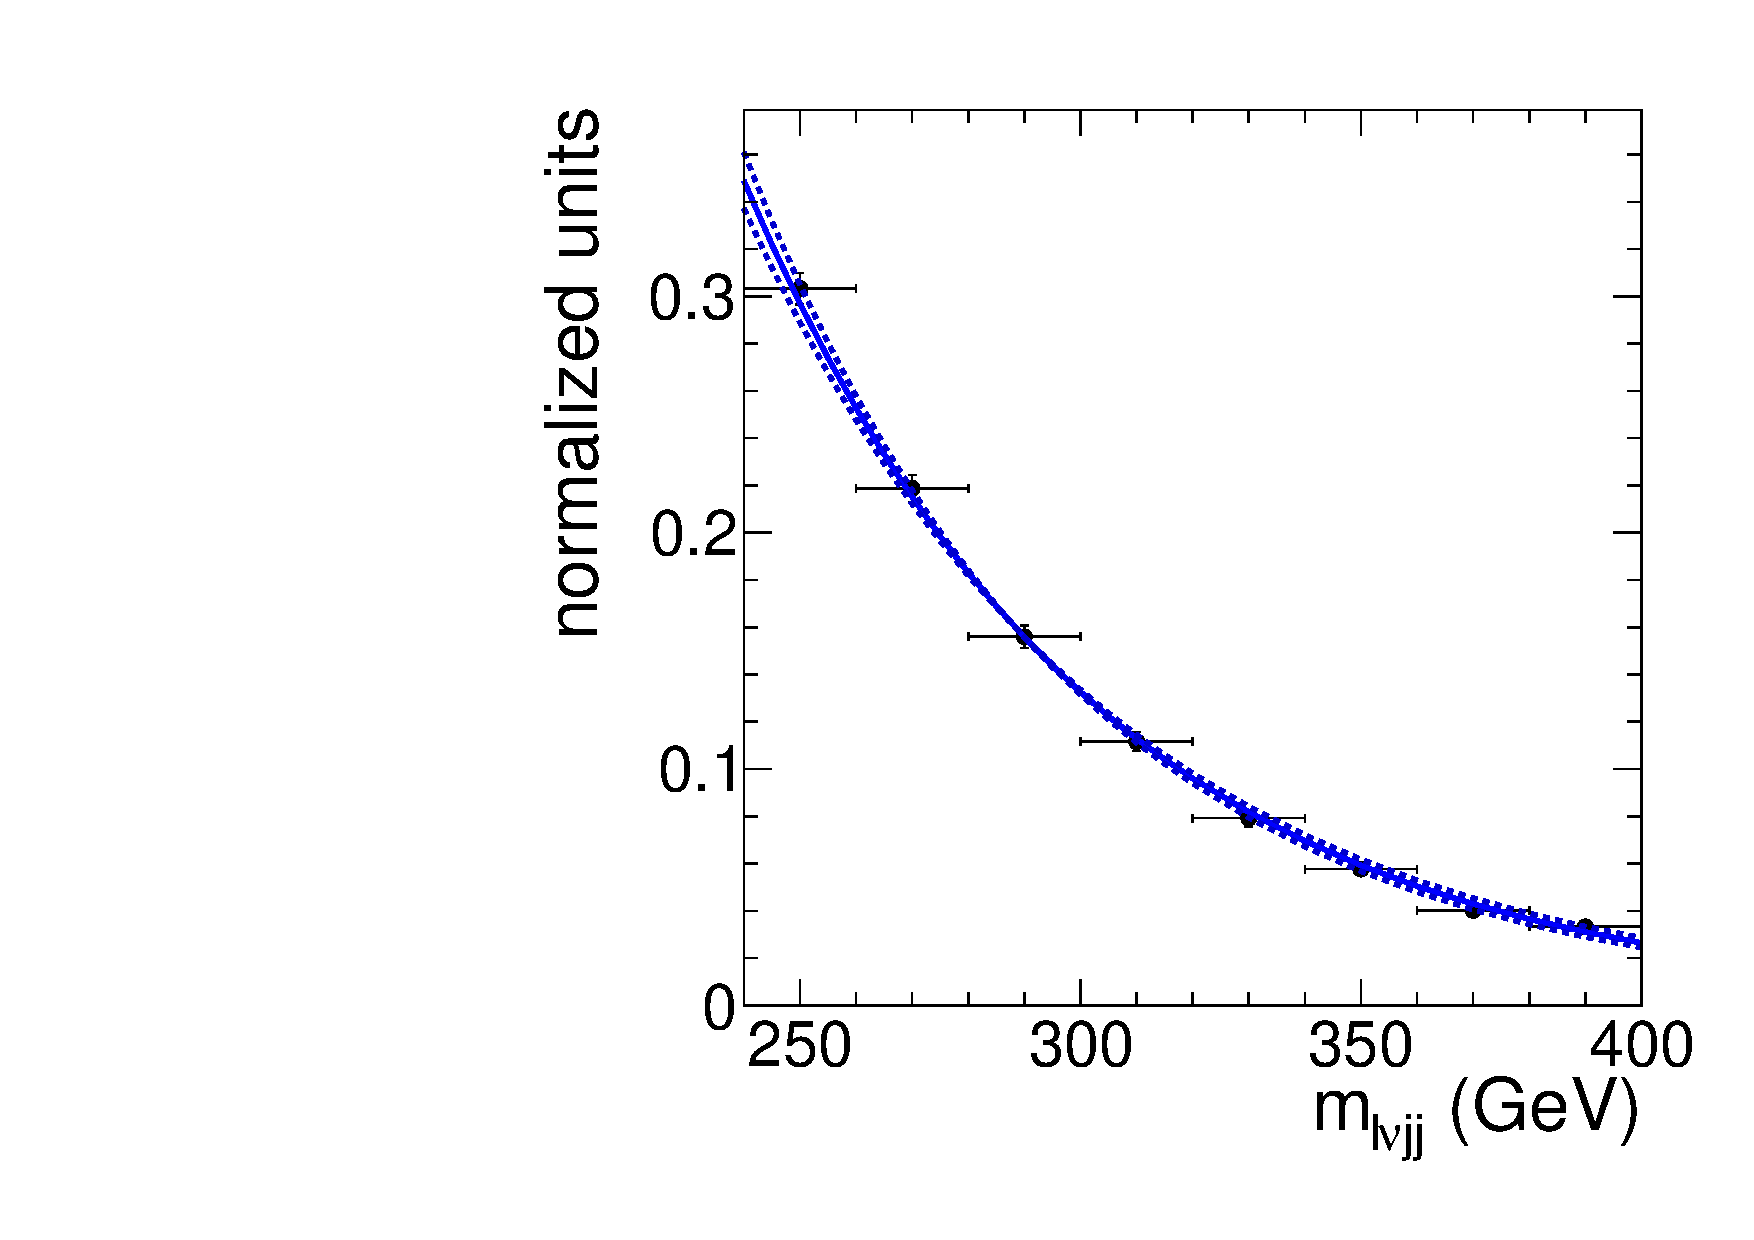
\includegraphics[width=0.49\textwidth]{plots/2012_WJetsShape/H300_Mlvjj_Muon_2jets_WpJShape.pdf}
    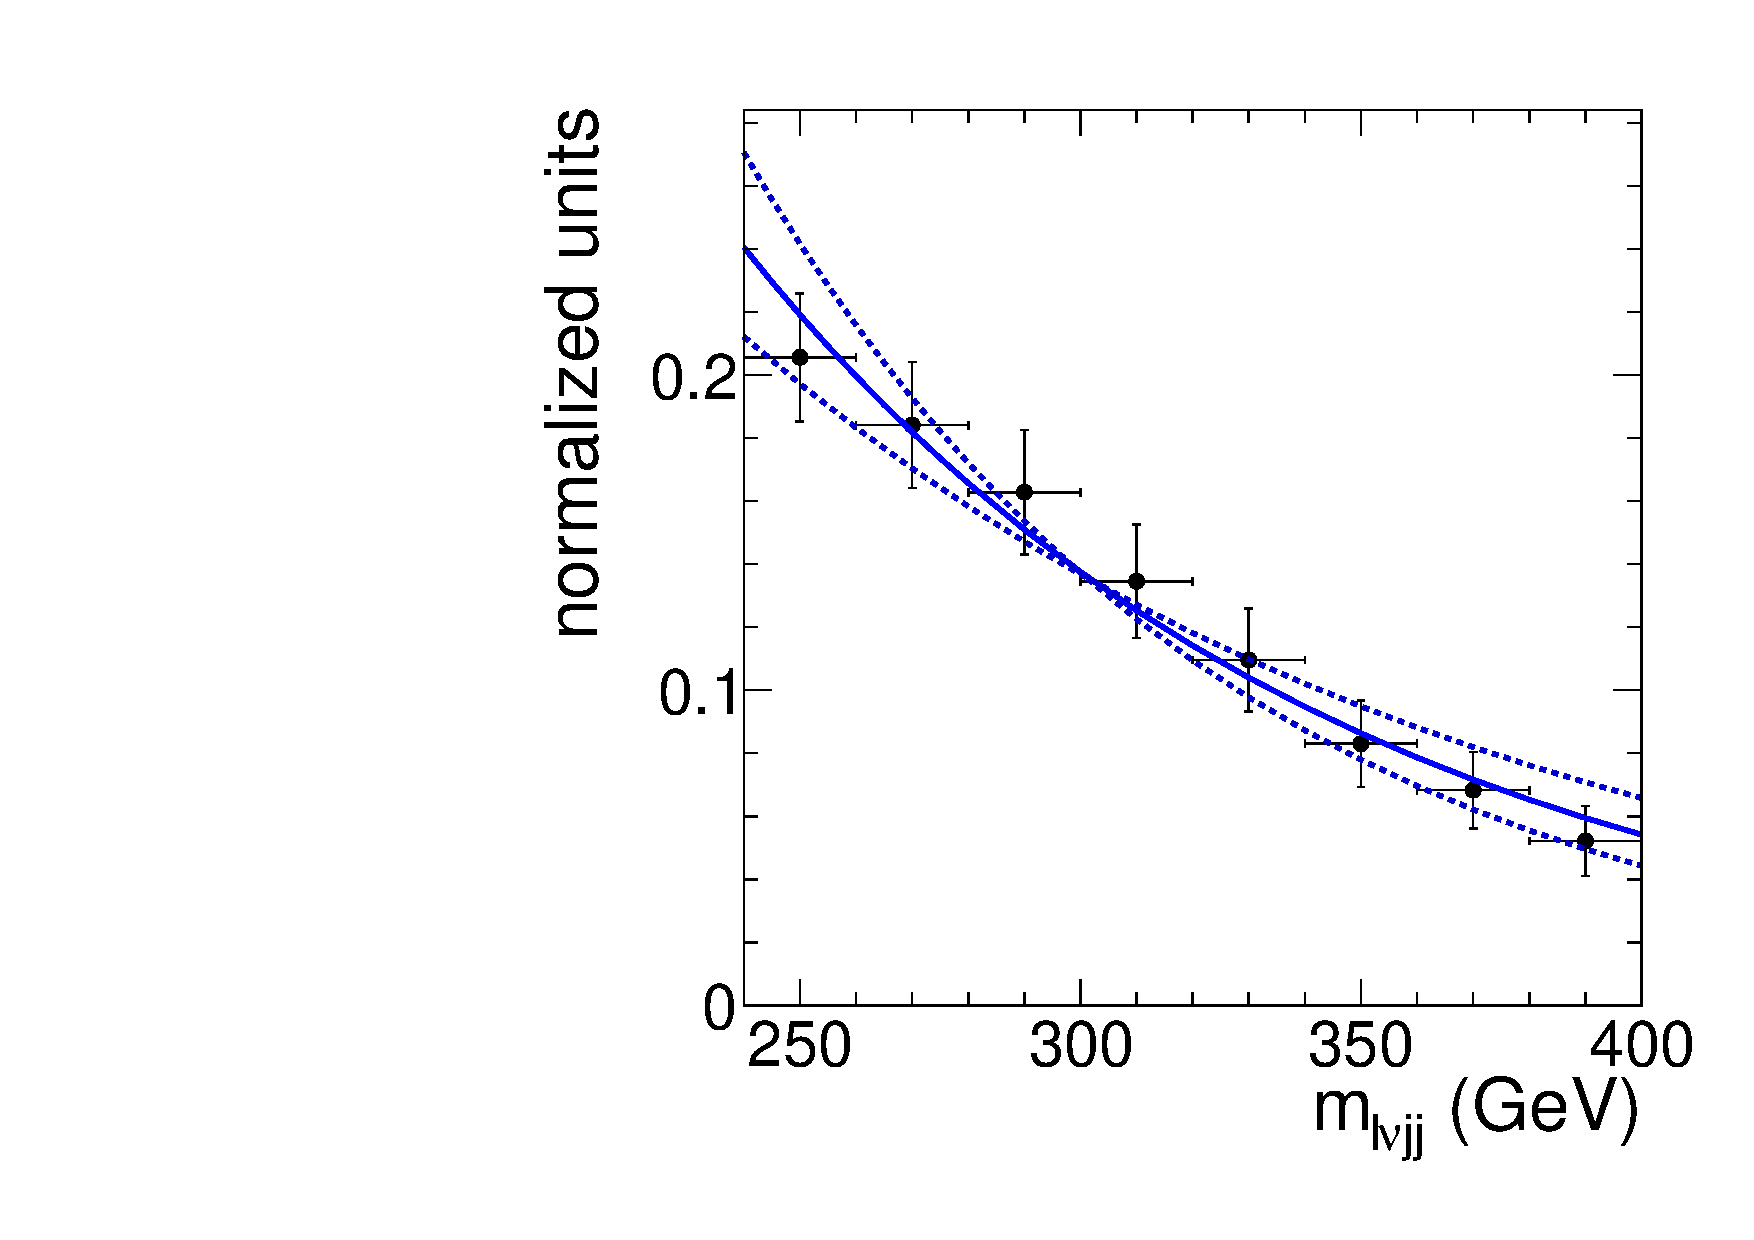
\includegraphics[width=0.49\textwidth]{plots/2012_WJetsShape/H300_Mlvjj_Electron_3jets_WpJShape.pdf}
    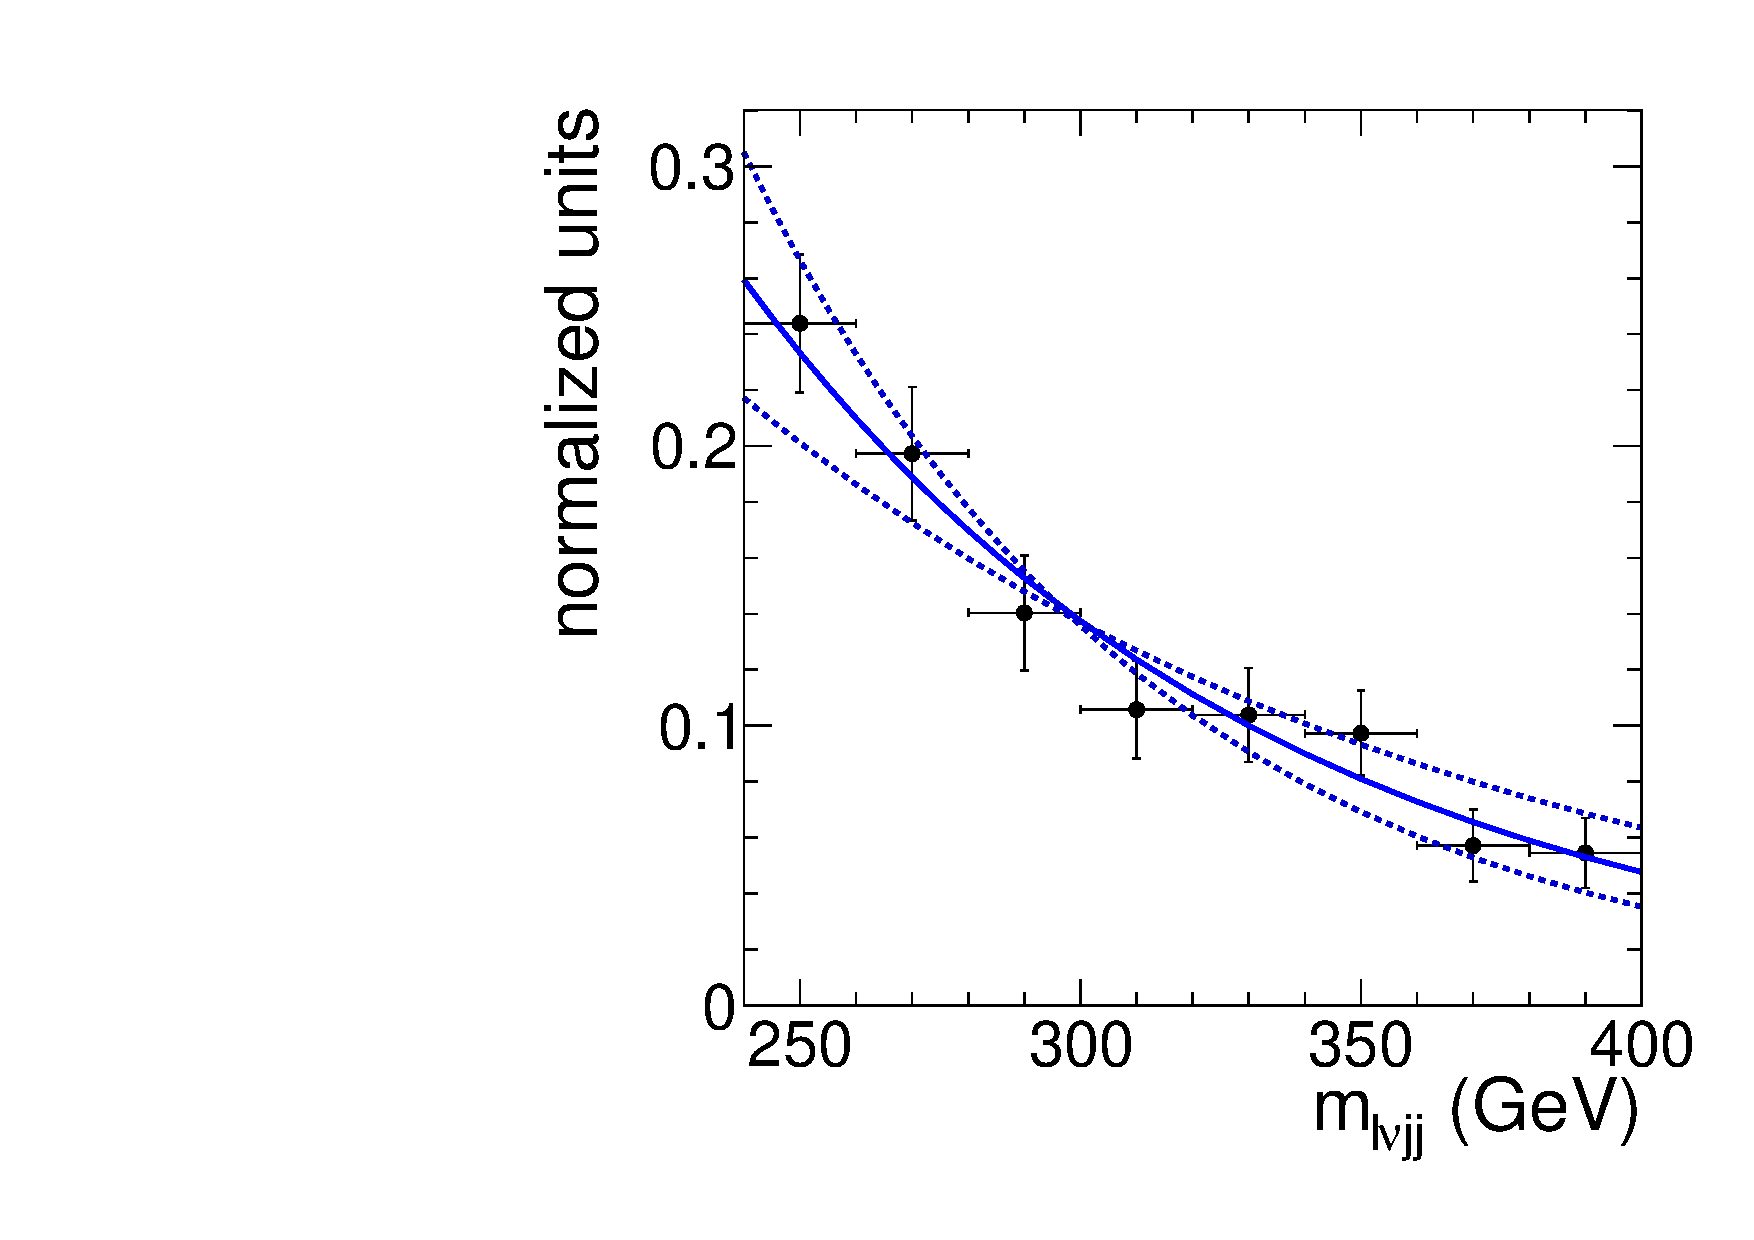
\includegraphics[width=0.49\textwidth]{plots/2012_WJetsShape/H300_Mlvjj_Muon_3jets_WpJShape.pdf}
  \caption{\label{fig:Wjets_dd_300}
  The distribution of the extrapolated background in the signal region
  is reported for the Higgs mass hypothesis of 300 GeV.
  On the top the 2 jets case, on the bottom the 3 jets case.
  Electrons are on the left, muons on the right.
  The points represent the extrapolated points, 
  while the red line shows the fitting function and the blue shaded band 
  the error from the fit.
    } 
\end{figure}
%
\begin{figure}[!t]
  \centering
    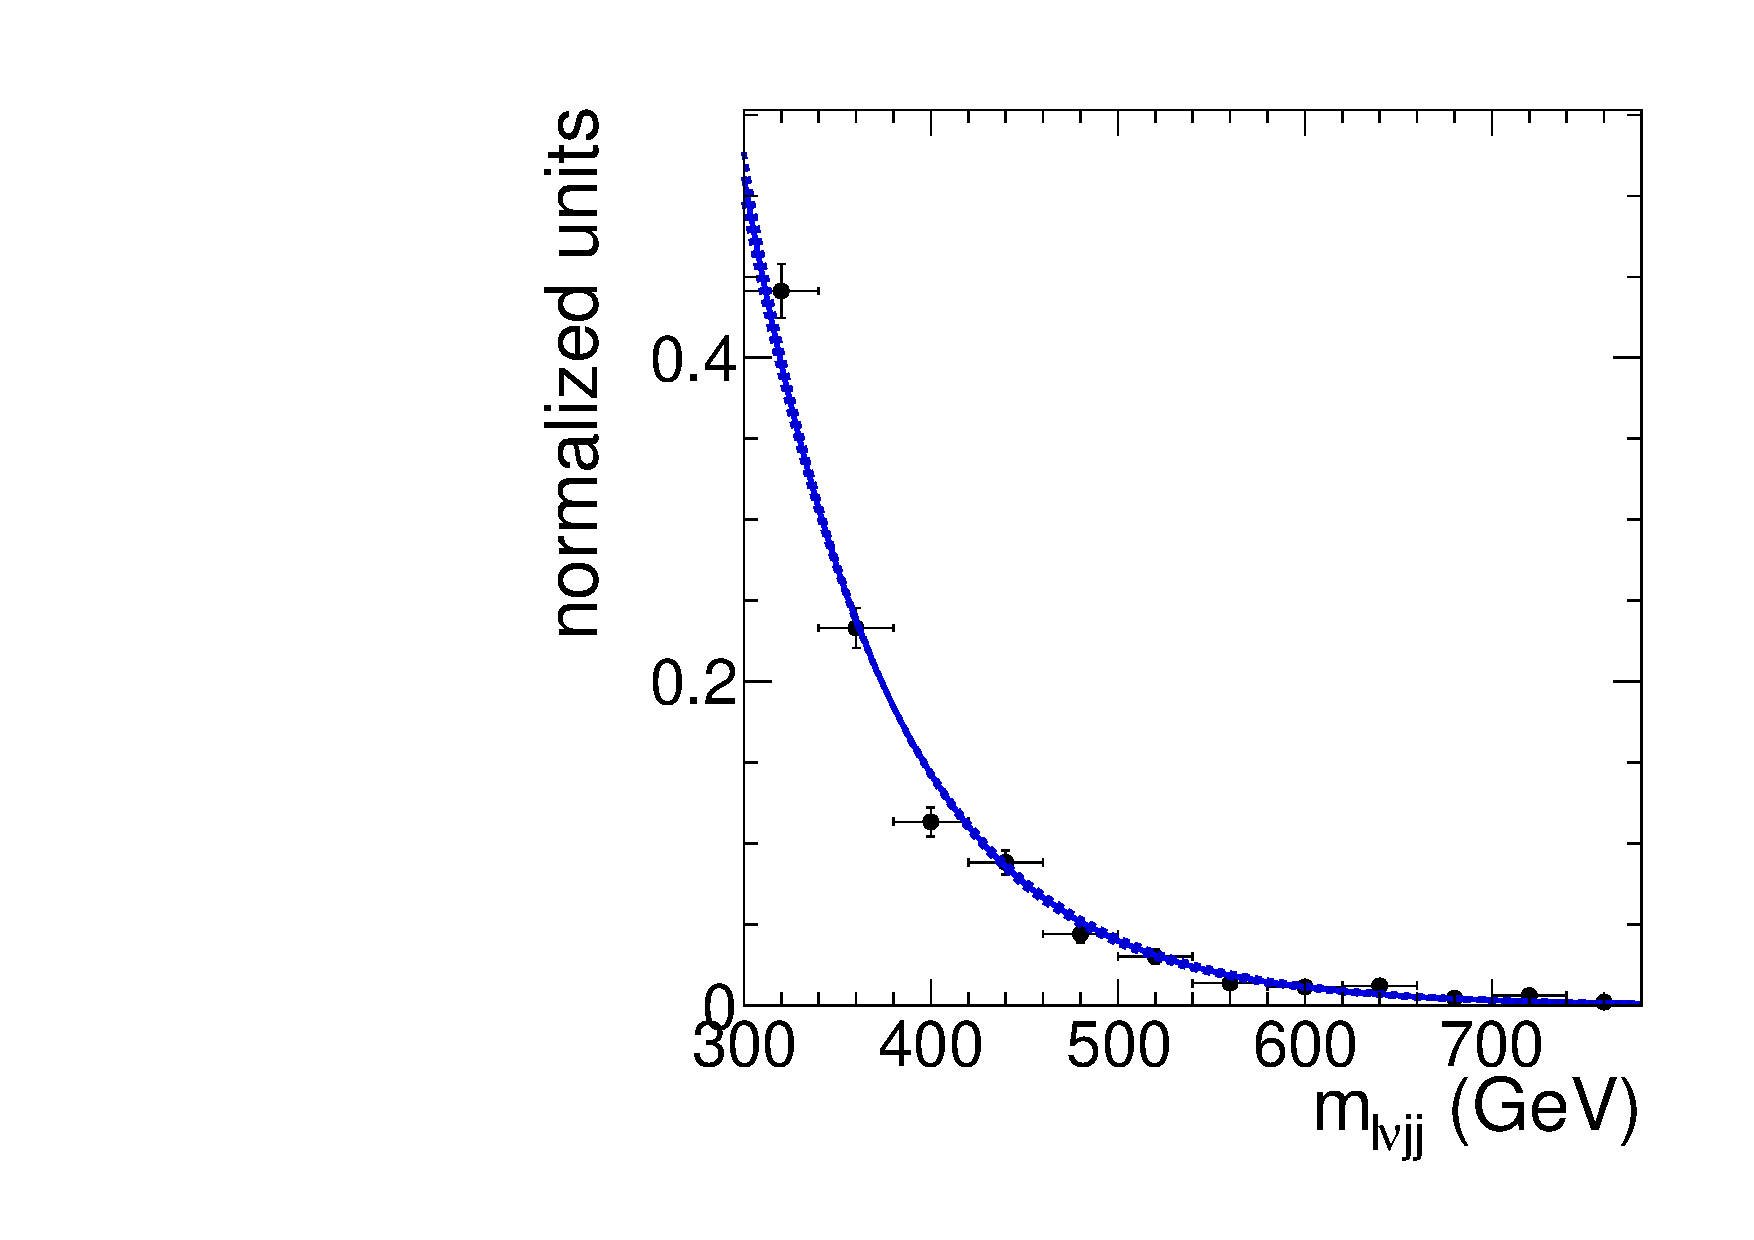
\includegraphics[width=0.49\textwidth]{plots/2012_WJetsShape/H350_Mlvjj_Electron_2jets_WpJShape.pdf}
    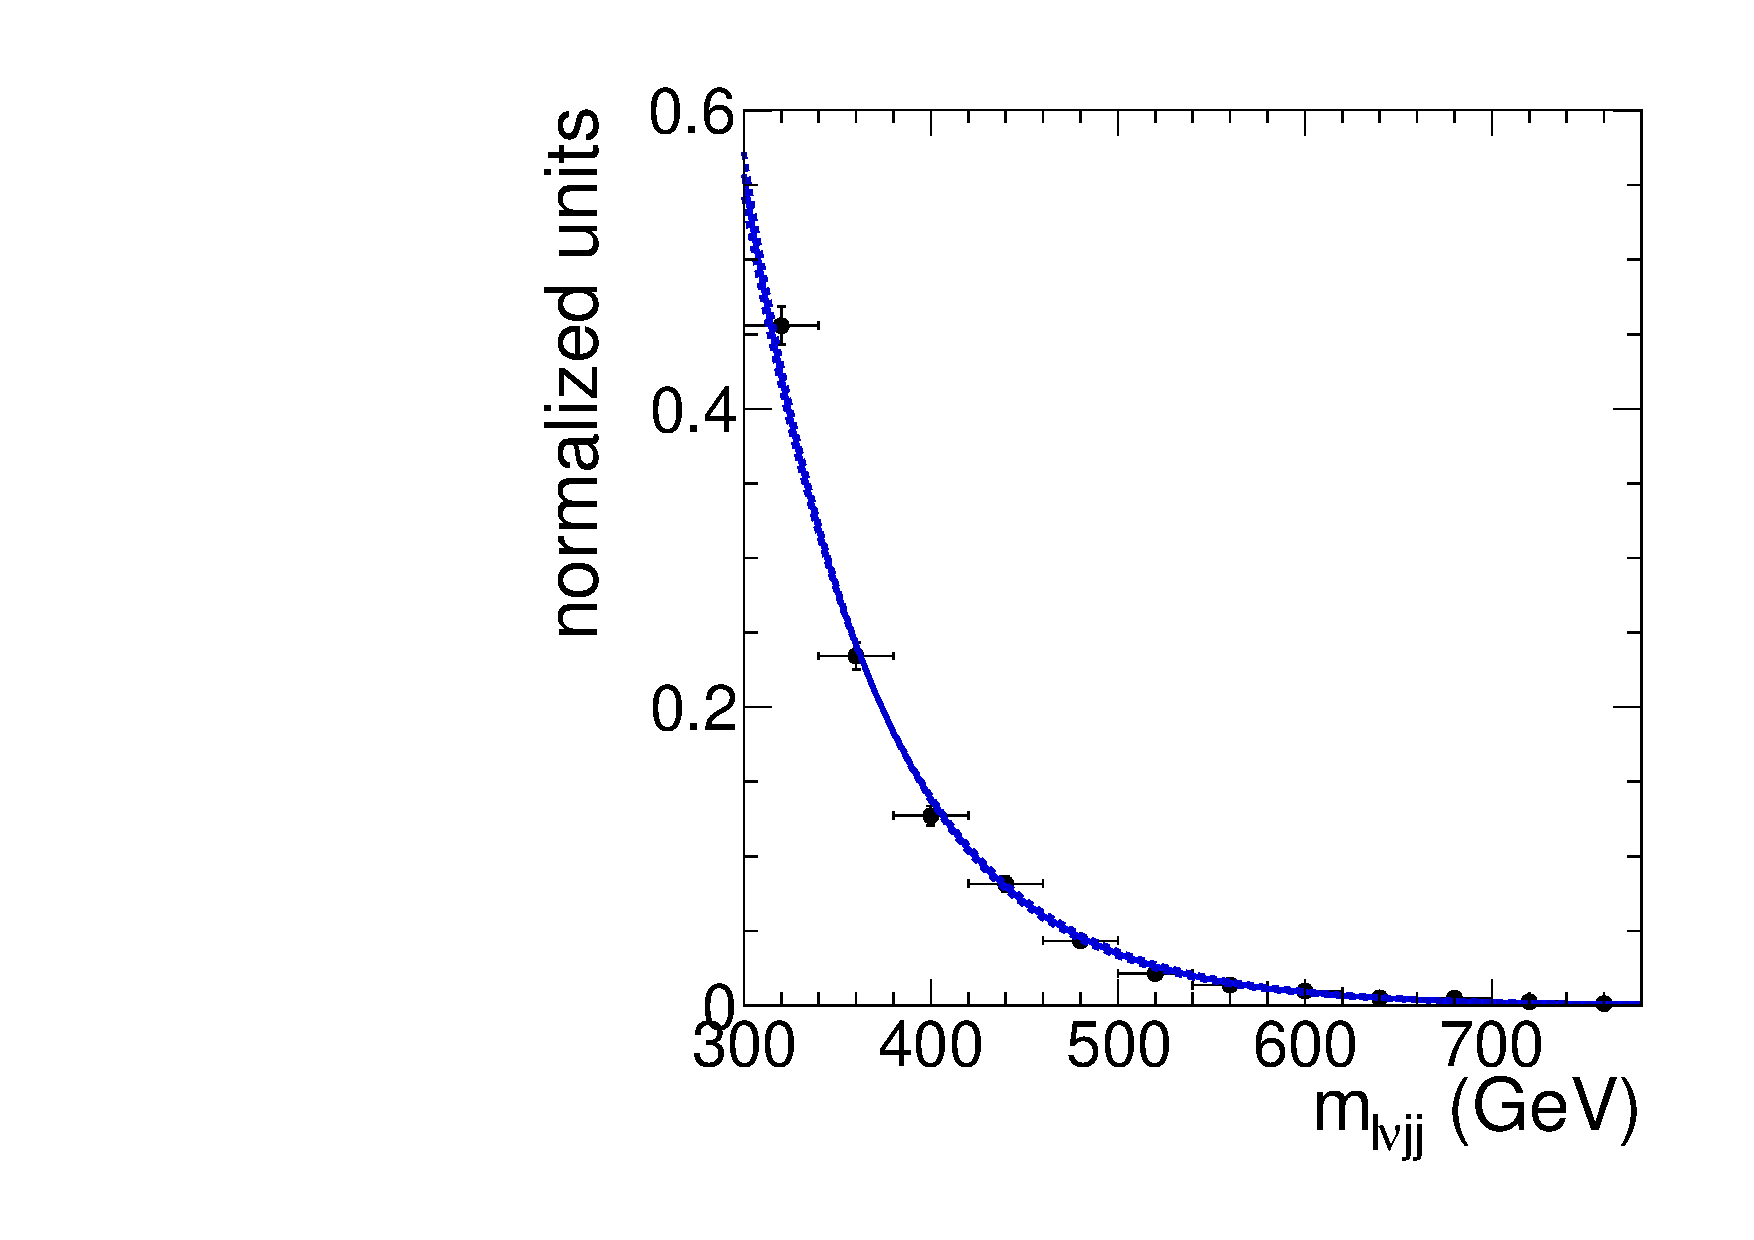
\includegraphics[width=0.49\textwidth]{plots/2012_WJetsShape/H350_Mlvjj_Muon_2jets_WpJShape.pdf}
    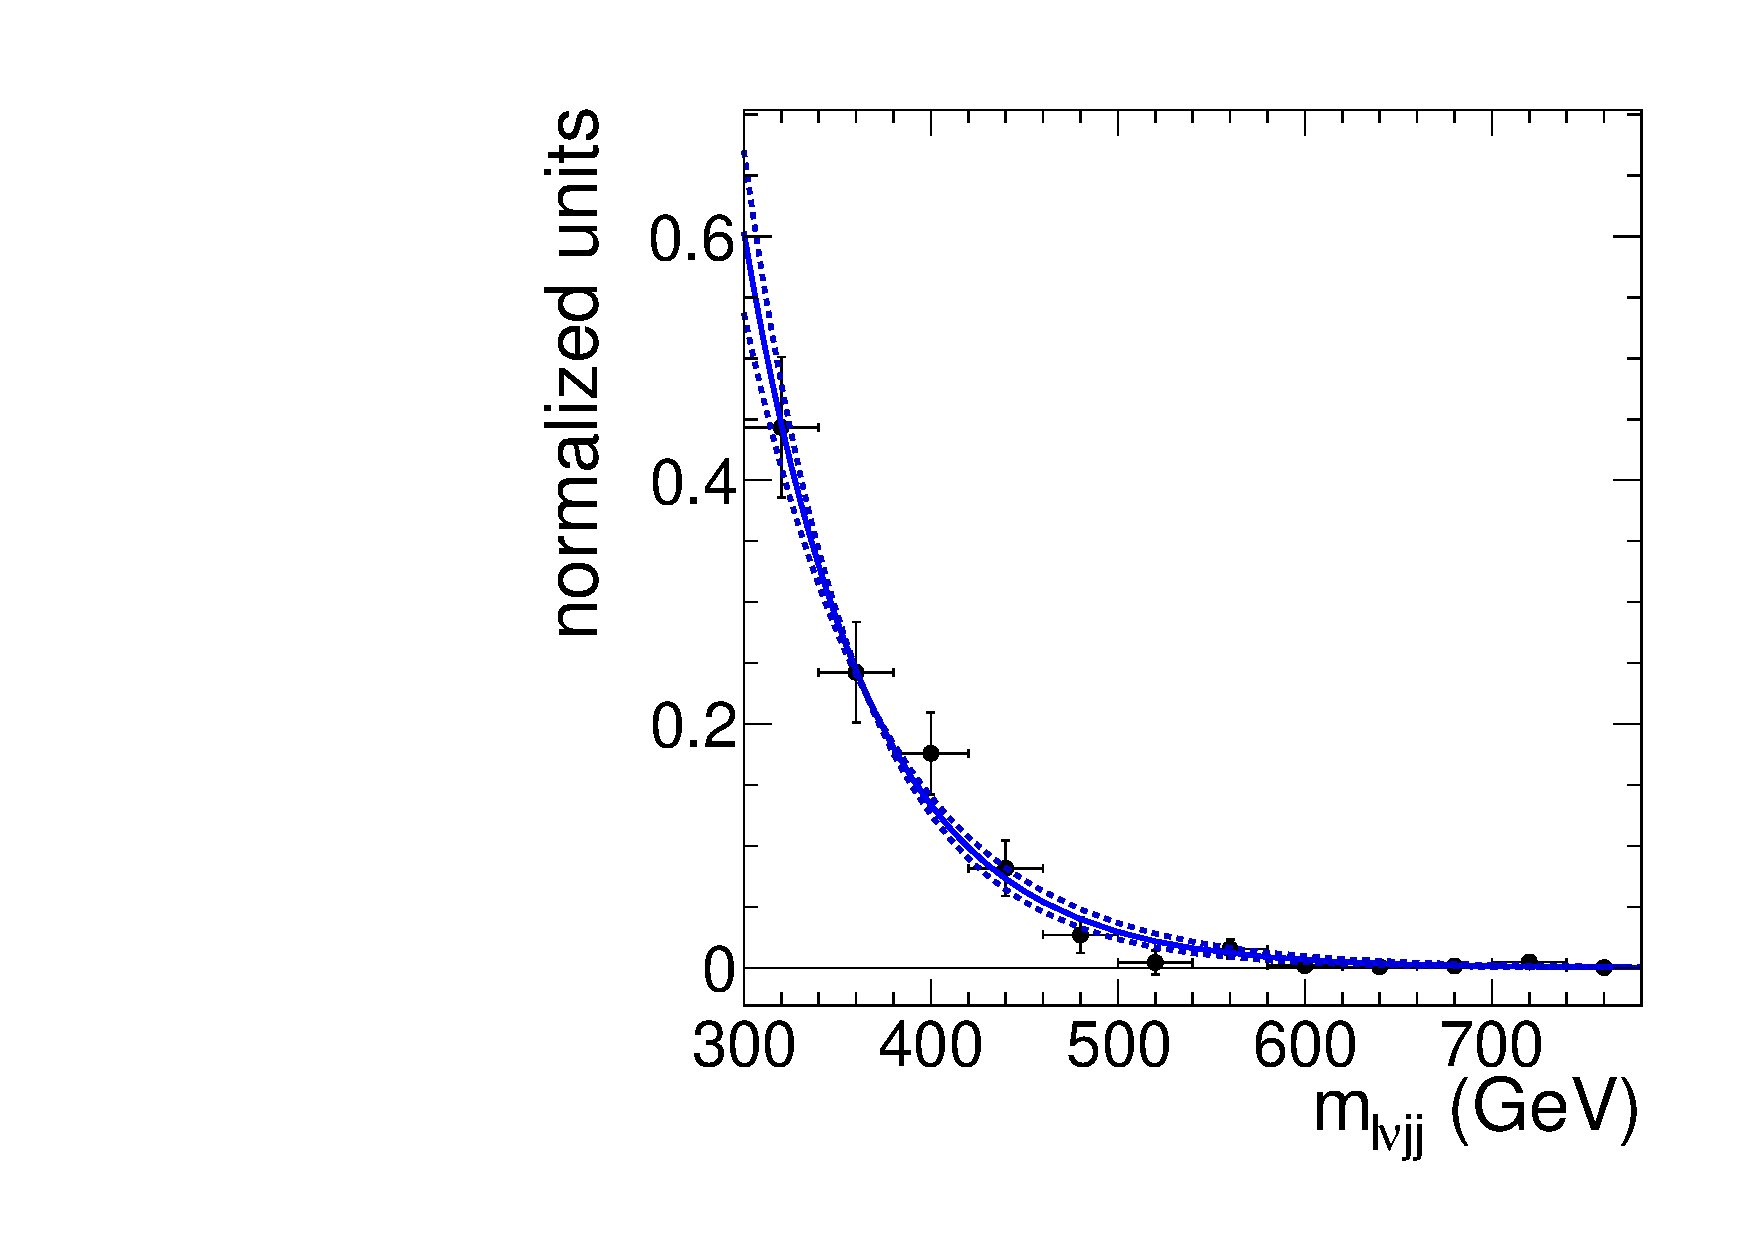
\includegraphics[width=0.49\textwidth]{plots/2012_WJetsShape/H350_Mlvjj_Electron_3jets_WpJShape.pdf}
    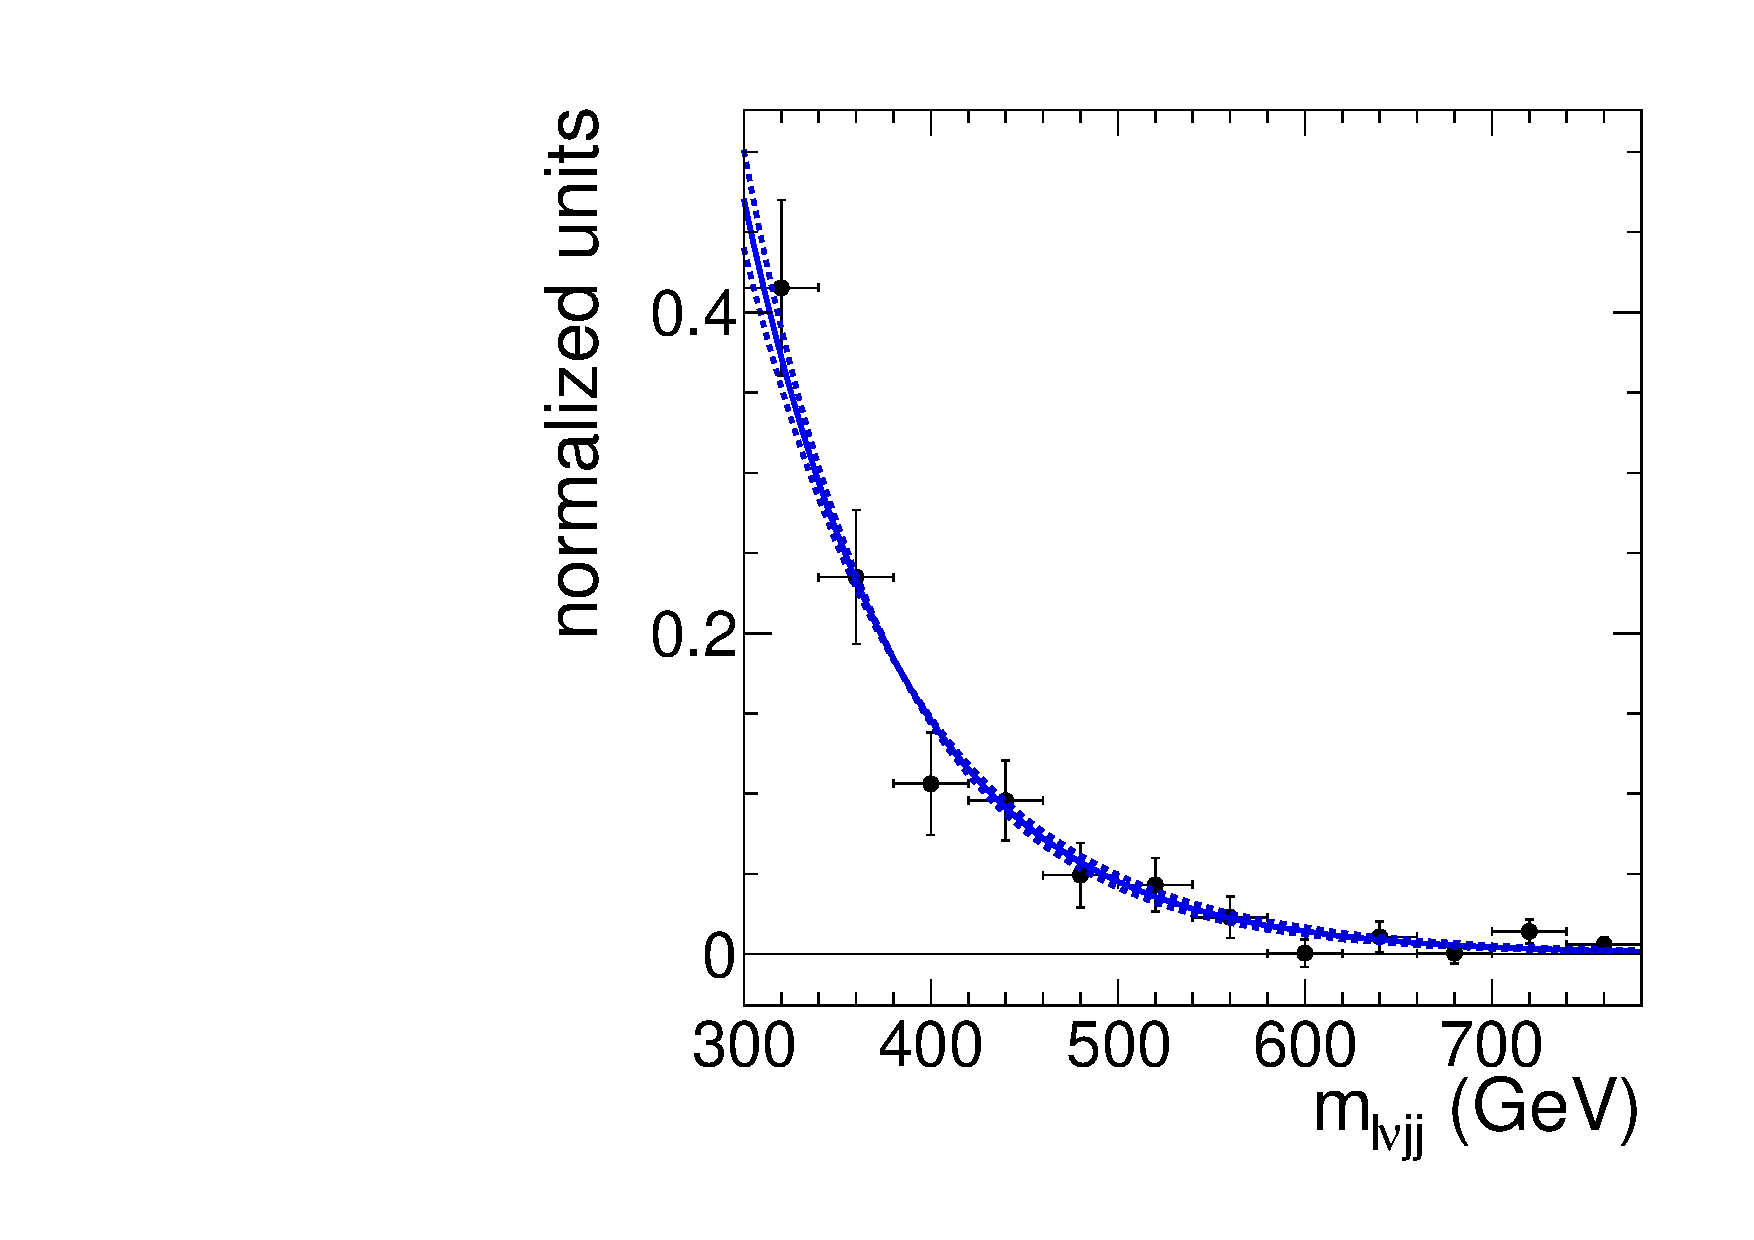
\includegraphics[width=0.49\textwidth]{plots/2012_WJetsShape/H350_Mlvjj_Muon_3jets_WpJShape.pdf}
  \caption{\label{fig:Wjets_dd_350}
  The distribution of the extrapolated background in the signal region
  is reported for the Higgs mass hypothesis of 350 GeV.
  On the top the 2 jets case, on the bottom the 3 jets case.
  Electrons are on the left, muons on the right.
  The points represent the extrapolated points, 
  while the red line shows the fitting function and the blue shaded band 
  the error from the fit.
    } 
\end{figure}
%
\begin{figure}[!t]
  \centering
    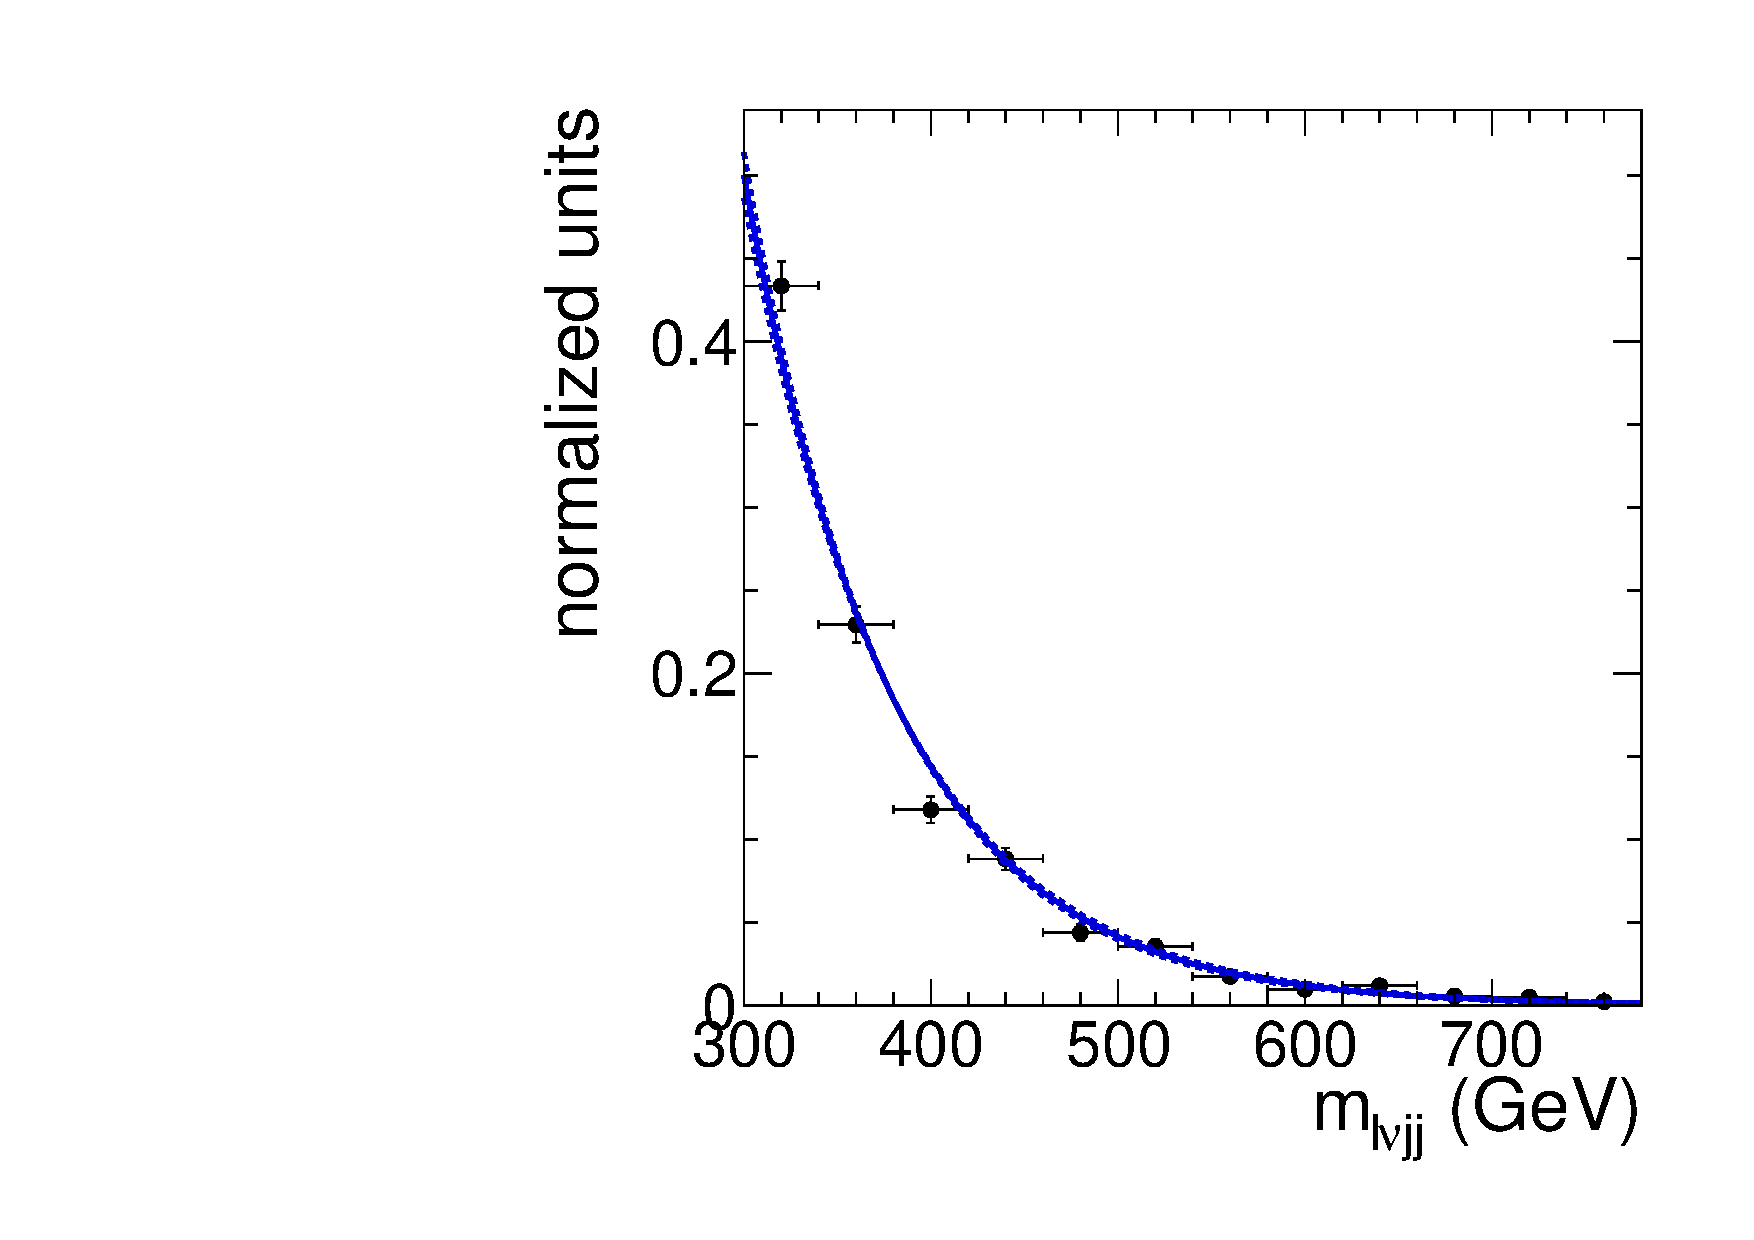
\includegraphics[width=0.49\textwidth]{plots/2012_WJetsShape/H400_Mlvjj_Electron_2jets_WpJShape.pdf}
    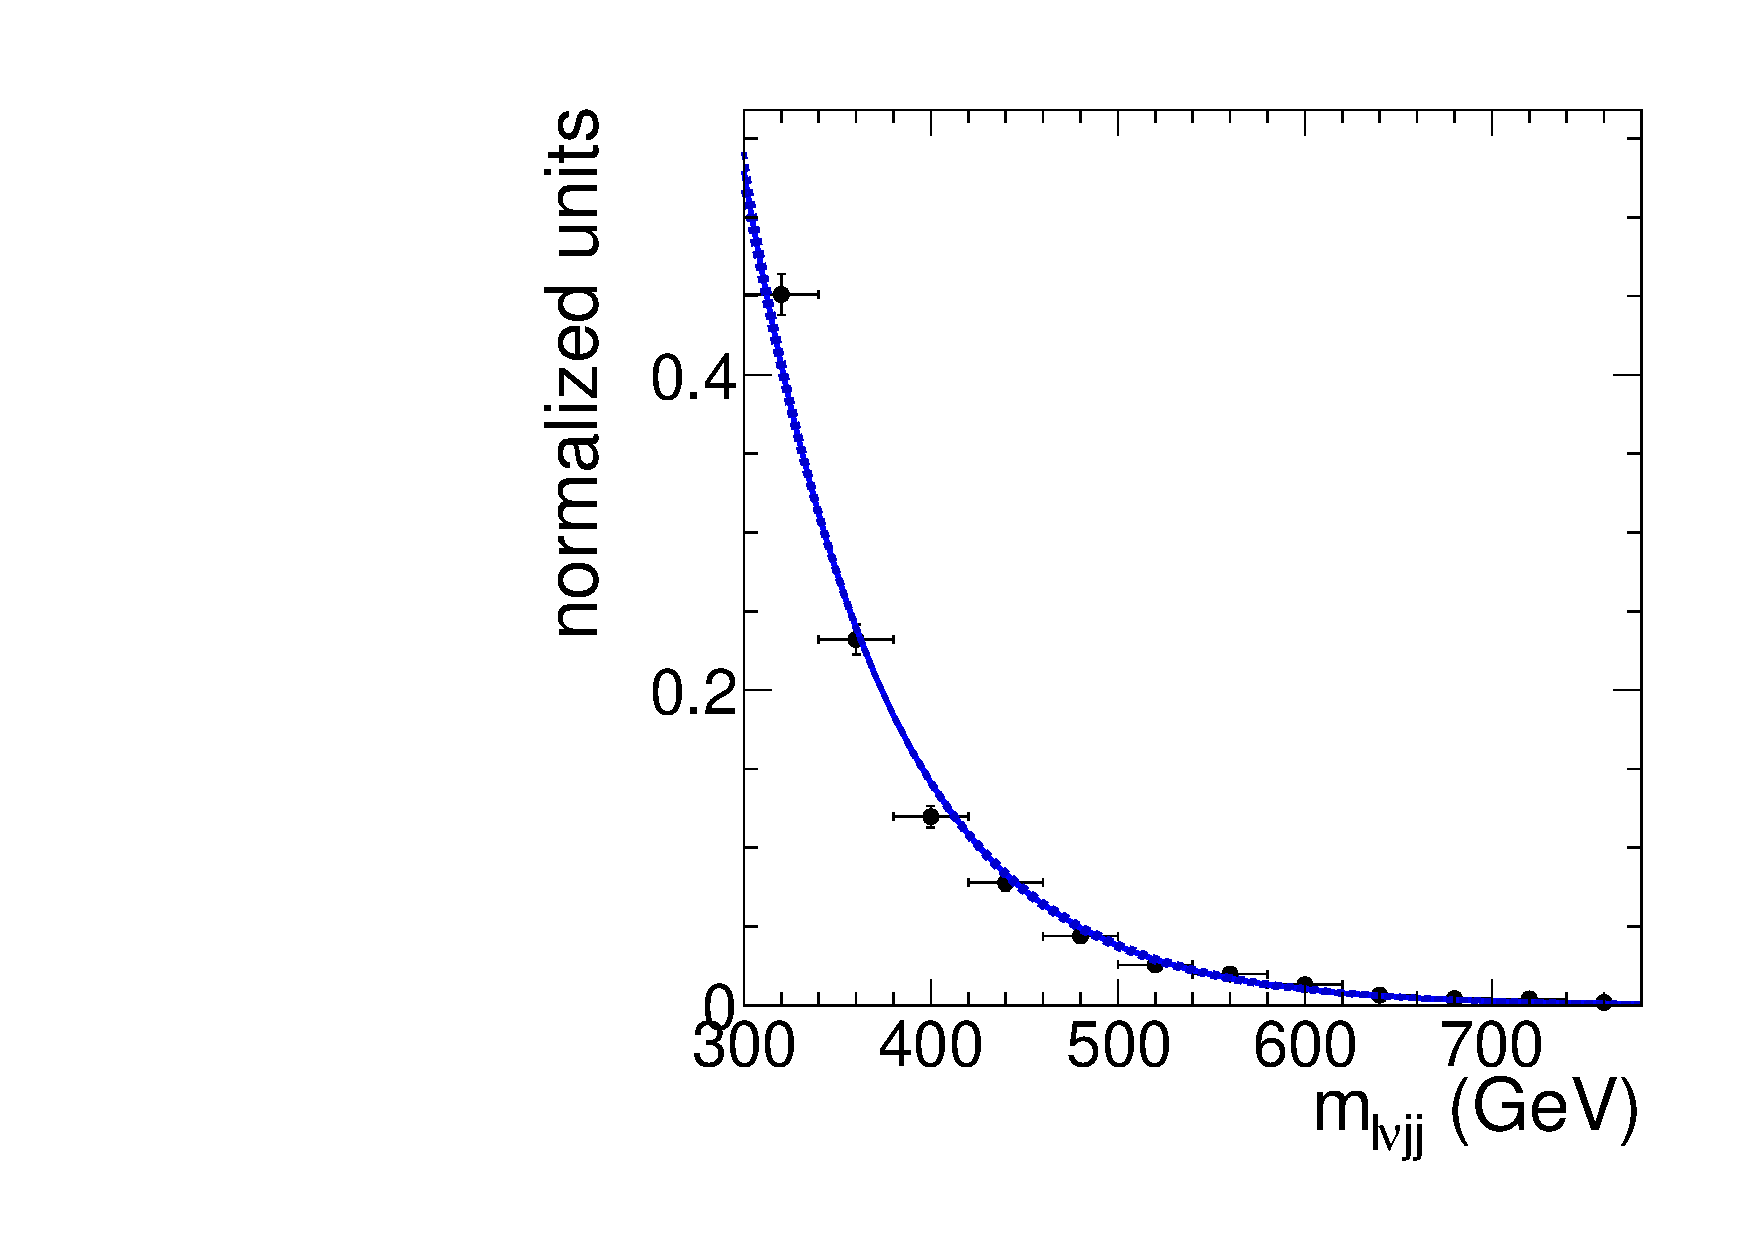
\includegraphics[width=0.49\textwidth]{plots/2012_WJetsShape/H400_Mlvjj_Muon_2jets_WpJShape.pdf}
    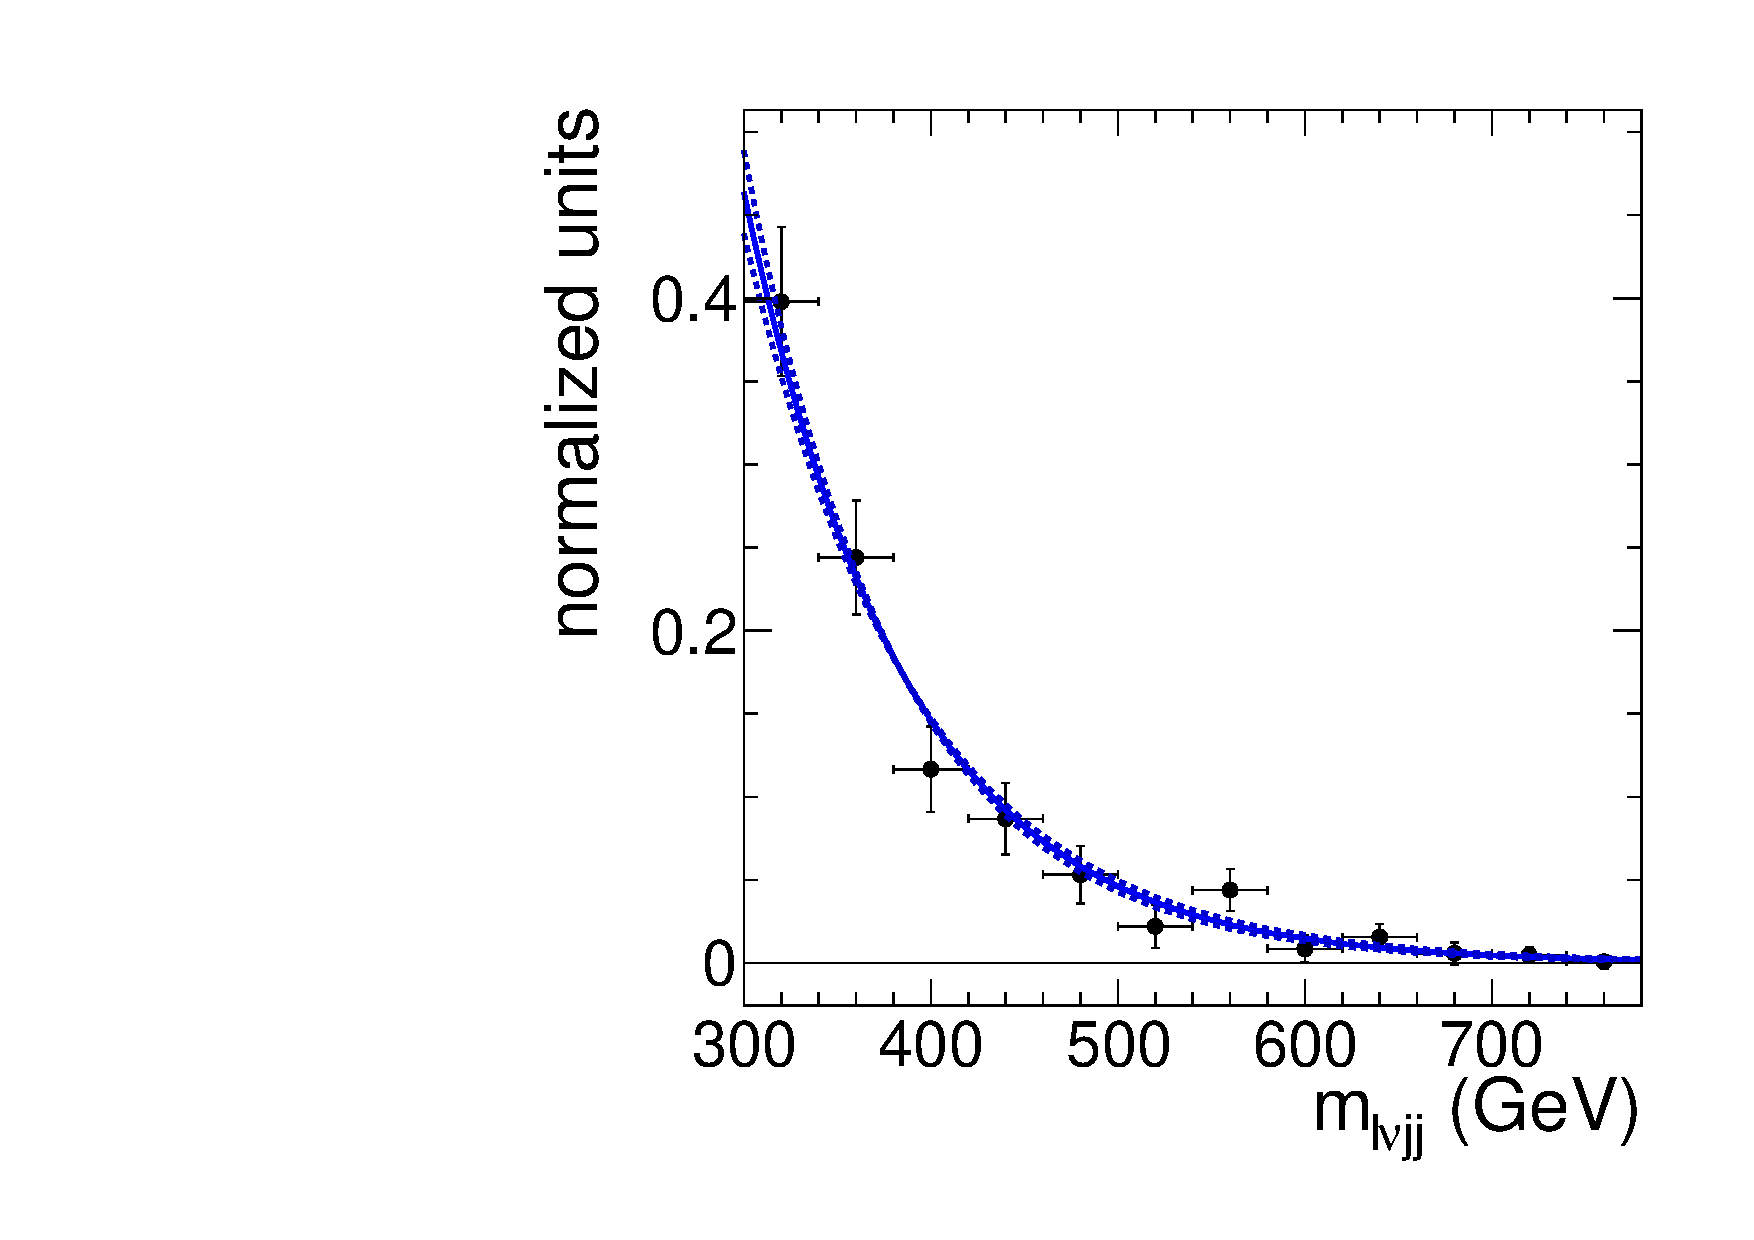
\includegraphics[width=0.49\textwidth]{plots/2012_WJetsShape/H400_Mlvjj_Electron_3jets_WpJShape.pdf}
    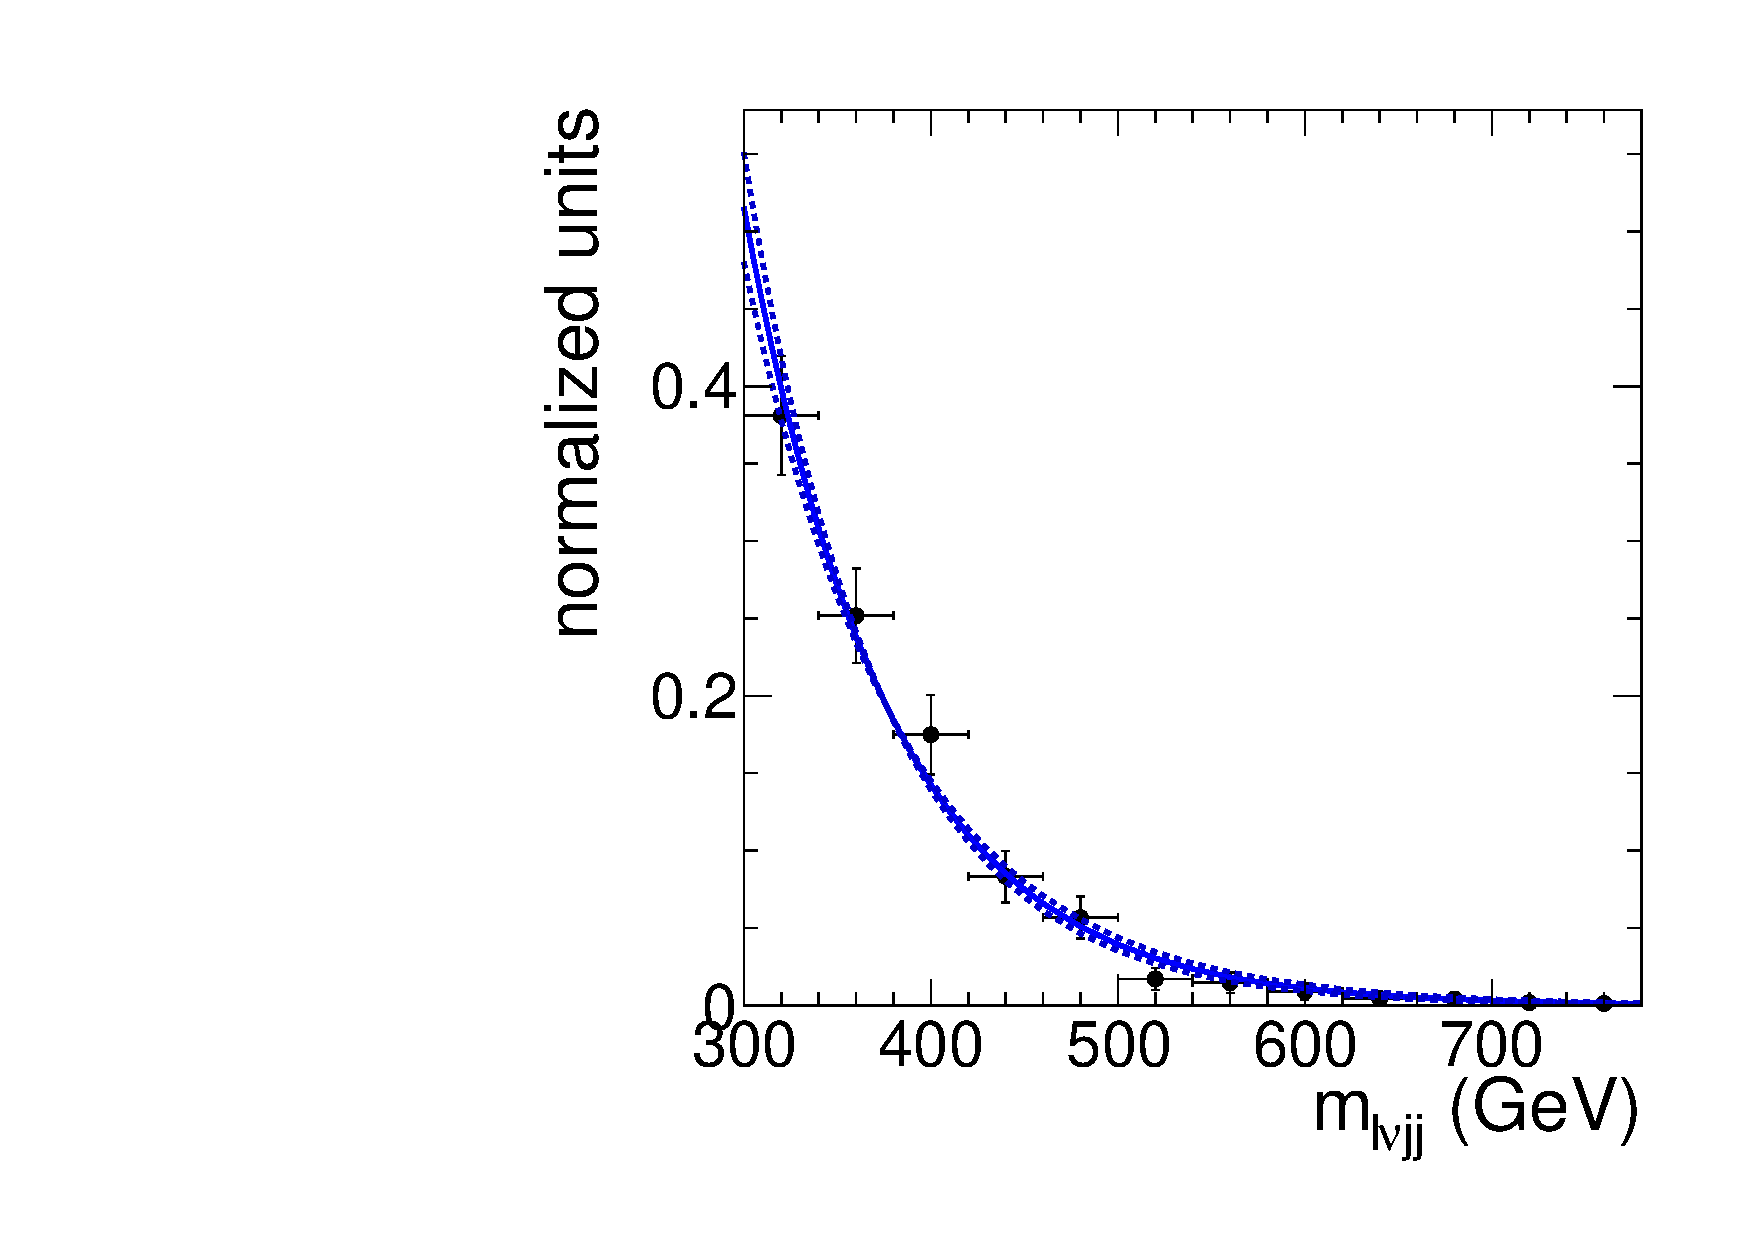
\includegraphics[width=0.49\textwidth]{plots/2012_WJetsShape/H400_Mlvjj_Muon_3jets_WpJShape.pdf}
  \caption{\label{fig:Wjets_dd_400}
  The distribution of the extrapolated background in the signal region
  is reported for the Higgs mass hypothesis of 400 GeV.
  On the top the 2 jets case, on the bottom the 3 jets case.
  Electrons are on the left, muons on the right.
  The points represent the extrapolated points, 
  while the red line shows the fitting function and the blue shaded band 
  the error from the fit.
    } 
\end{figure}
%
\begin{figure}[!t]
  \centering
    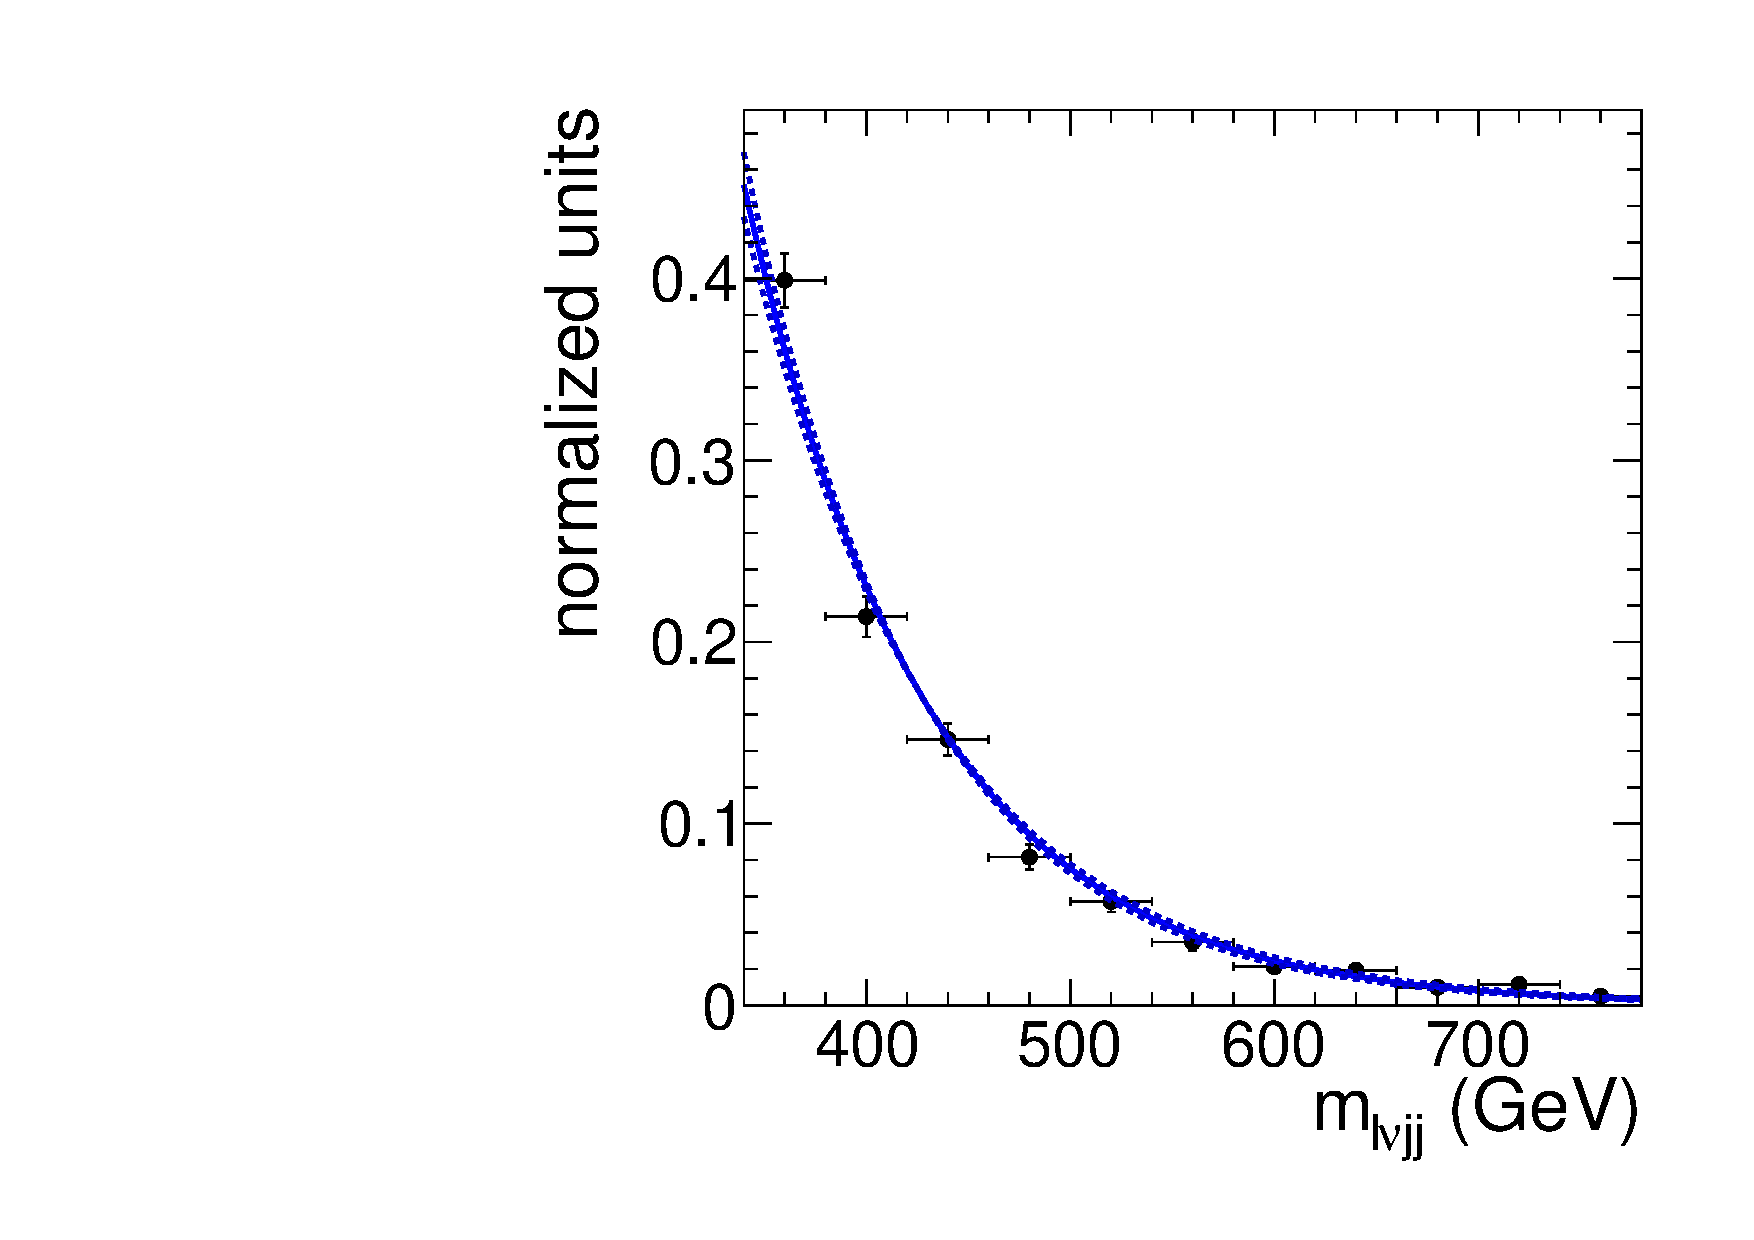
\includegraphics[width=0.49\textwidth]{plots/2012_WJetsShape/H450_Mlvjj_Electron_2jets_WpJShape.pdf}
    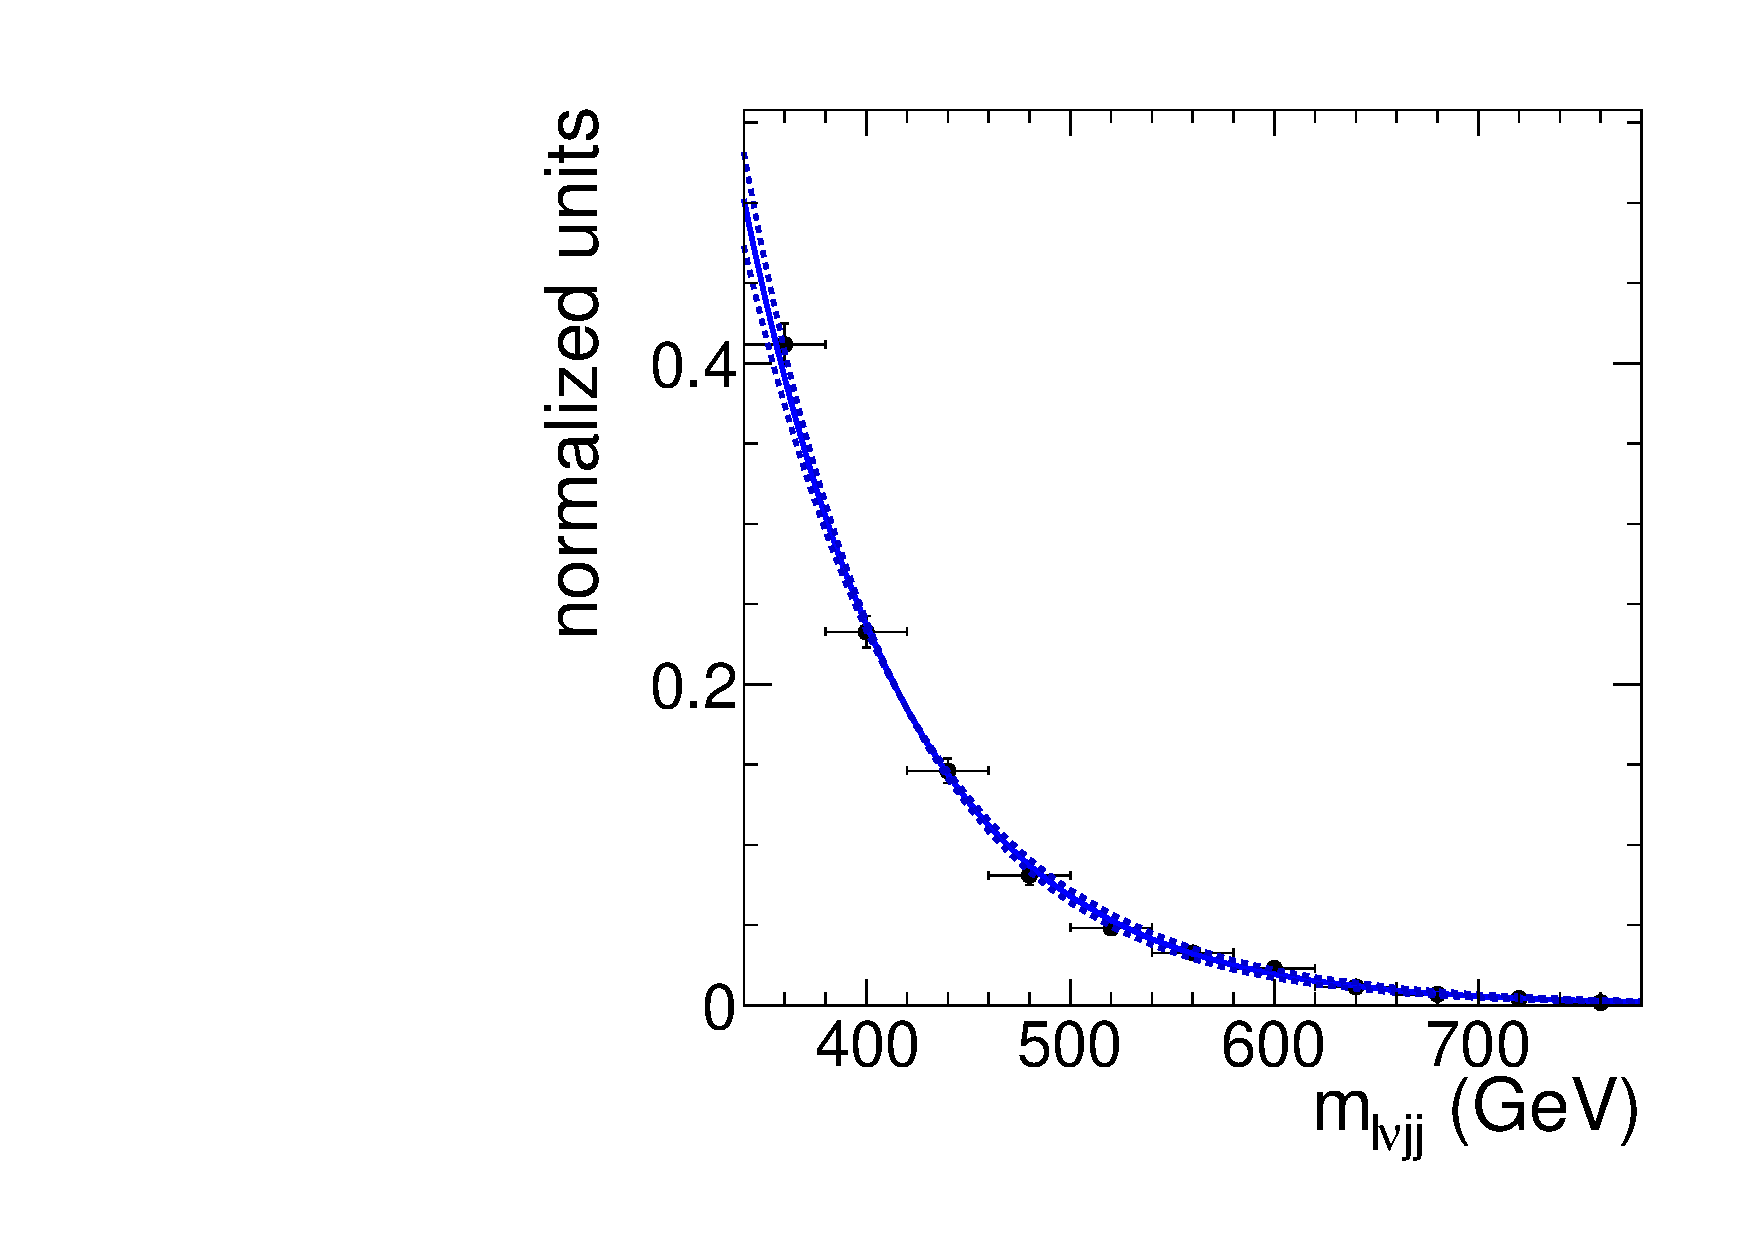
\includegraphics[width=0.49\textwidth]{plots/2012_WJetsShape/H450_Mlvjj_Muon_2jets_WpJShape.pdf}
    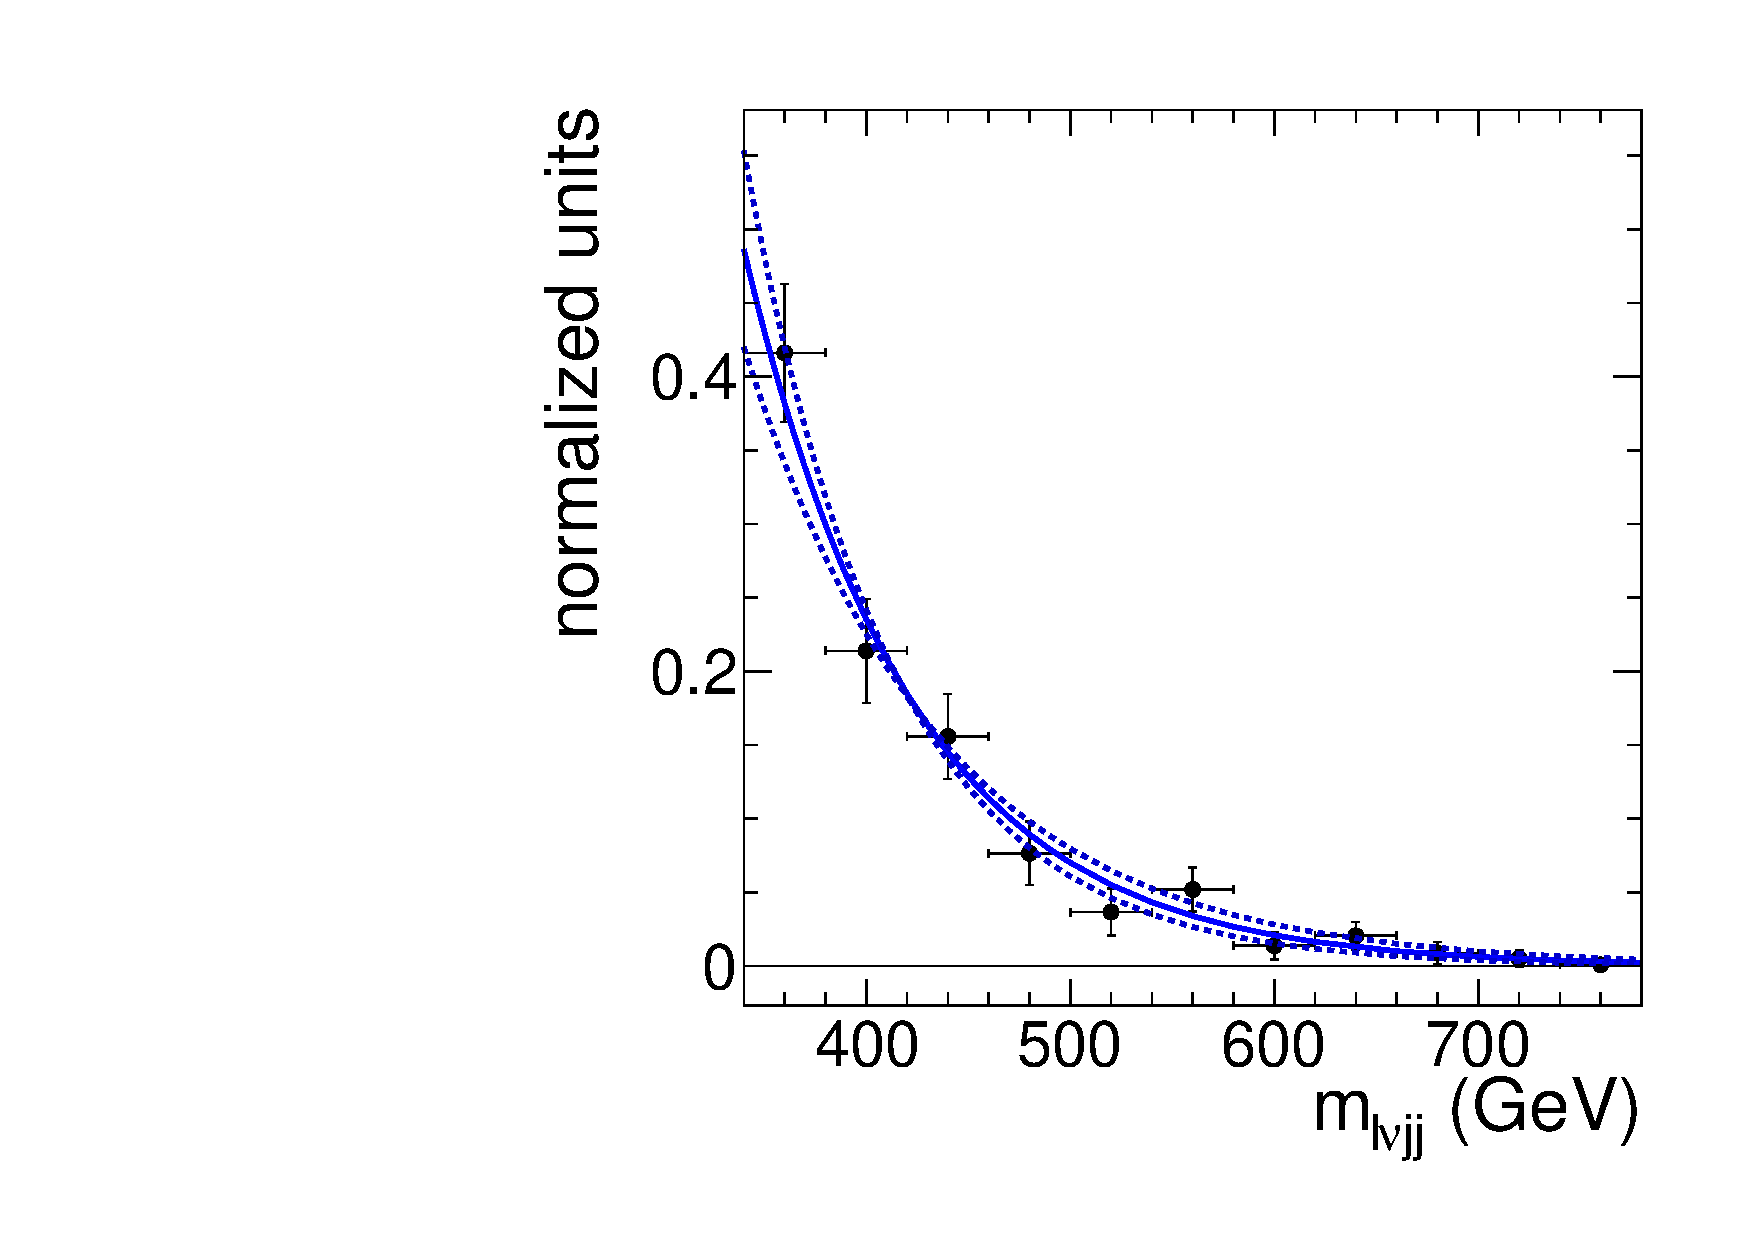
\includegraphics[width=0.49\textwidth]{plots/2012_WJetsShape/H450_Mlvjj_Electron_3jets_WpJShape.pdf}
    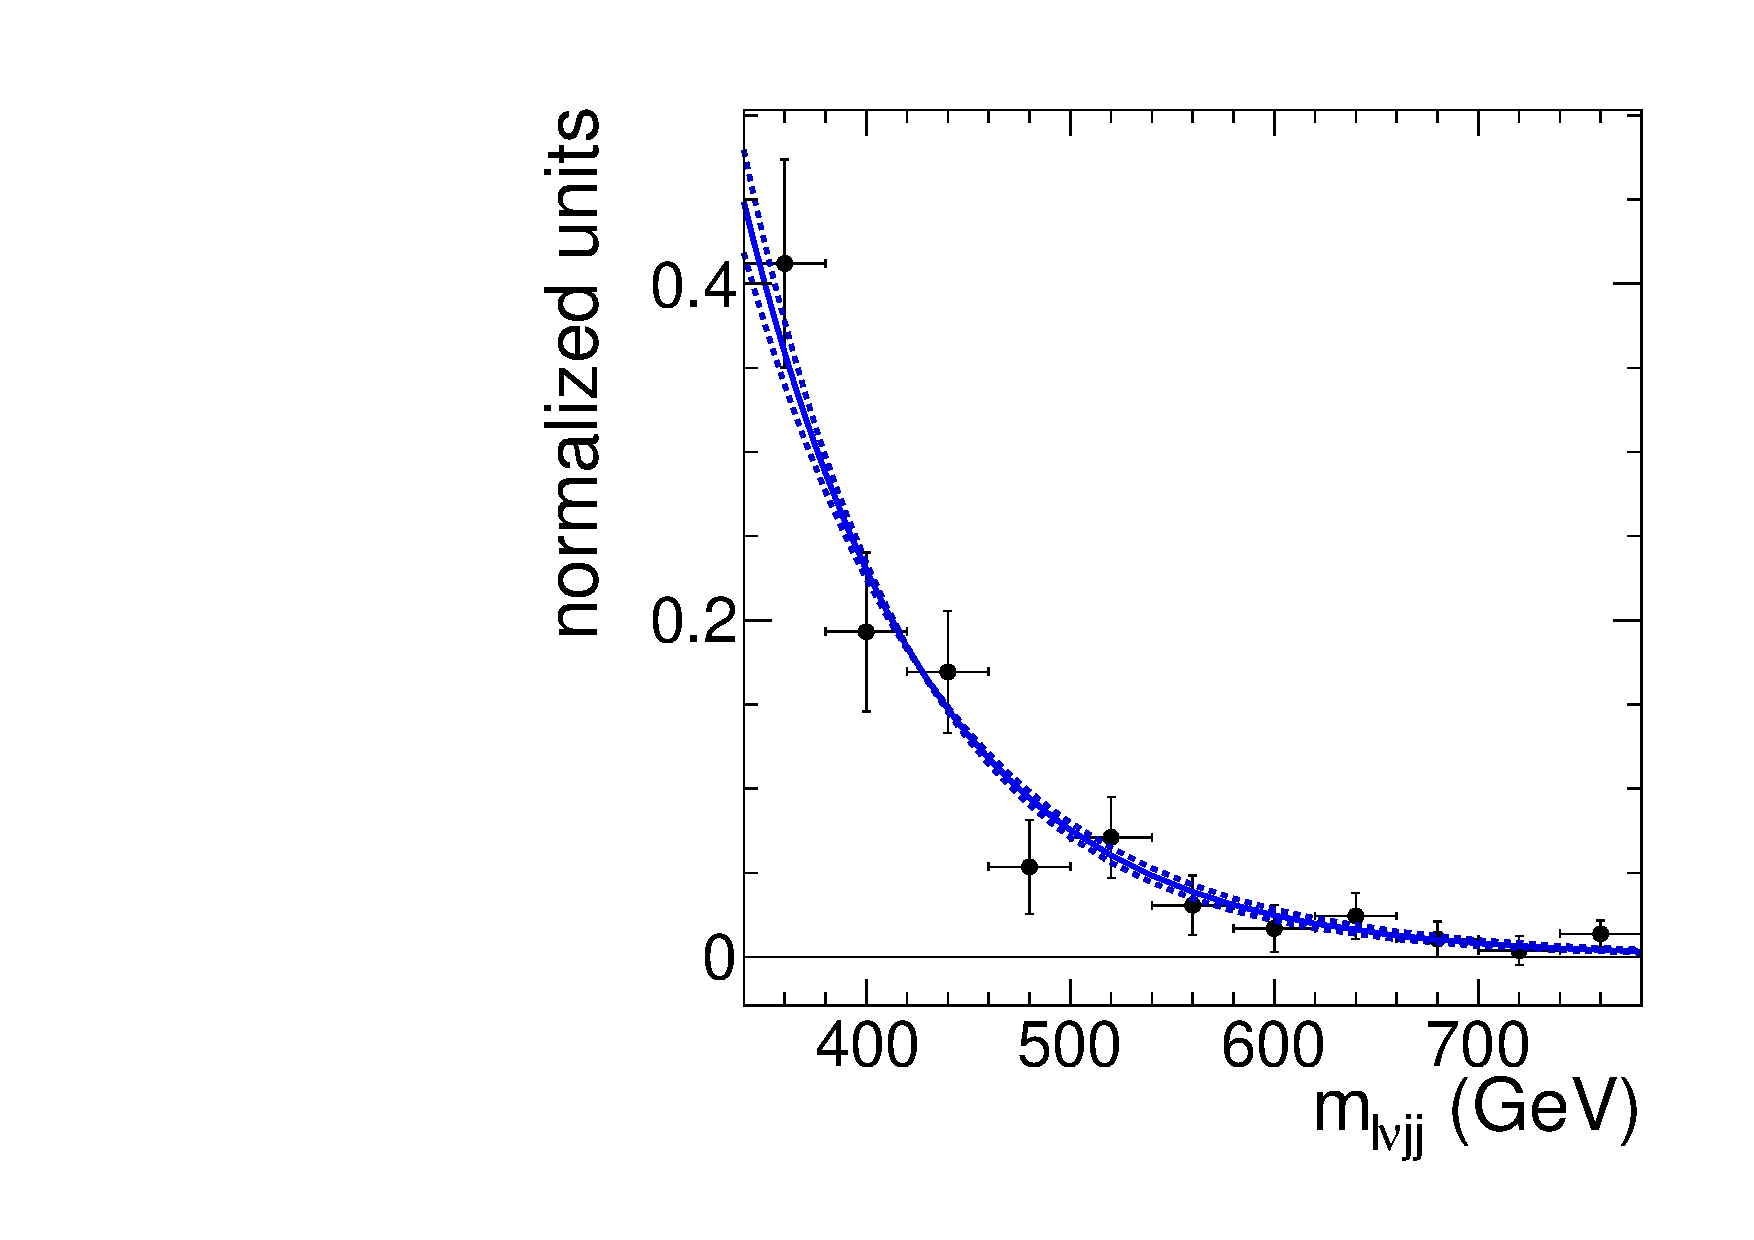
\includegraphics[width=0.49\textwidth]{plots/2012_WJetsShape/H450_Mlvjj_Muon_3jets_WpJShape.pdf}
  \caption{\label{fig:Wjets_dd_450}
  The distribution of the extrapolated background in the signal region
  is reported for the Higgs mass hypothesis of 450 GeV.
  On the top the 2 jets case, on the bottom the 3 jets case.
  Electrons are on the left, muons on the right.
  The points represent the extrapolated points, 
  while the red line shows the fitting function and the blue shaded band 
  the error from the fit.
    } 
\end{figure}
%
\begin{figure}[!t]
  \centering
    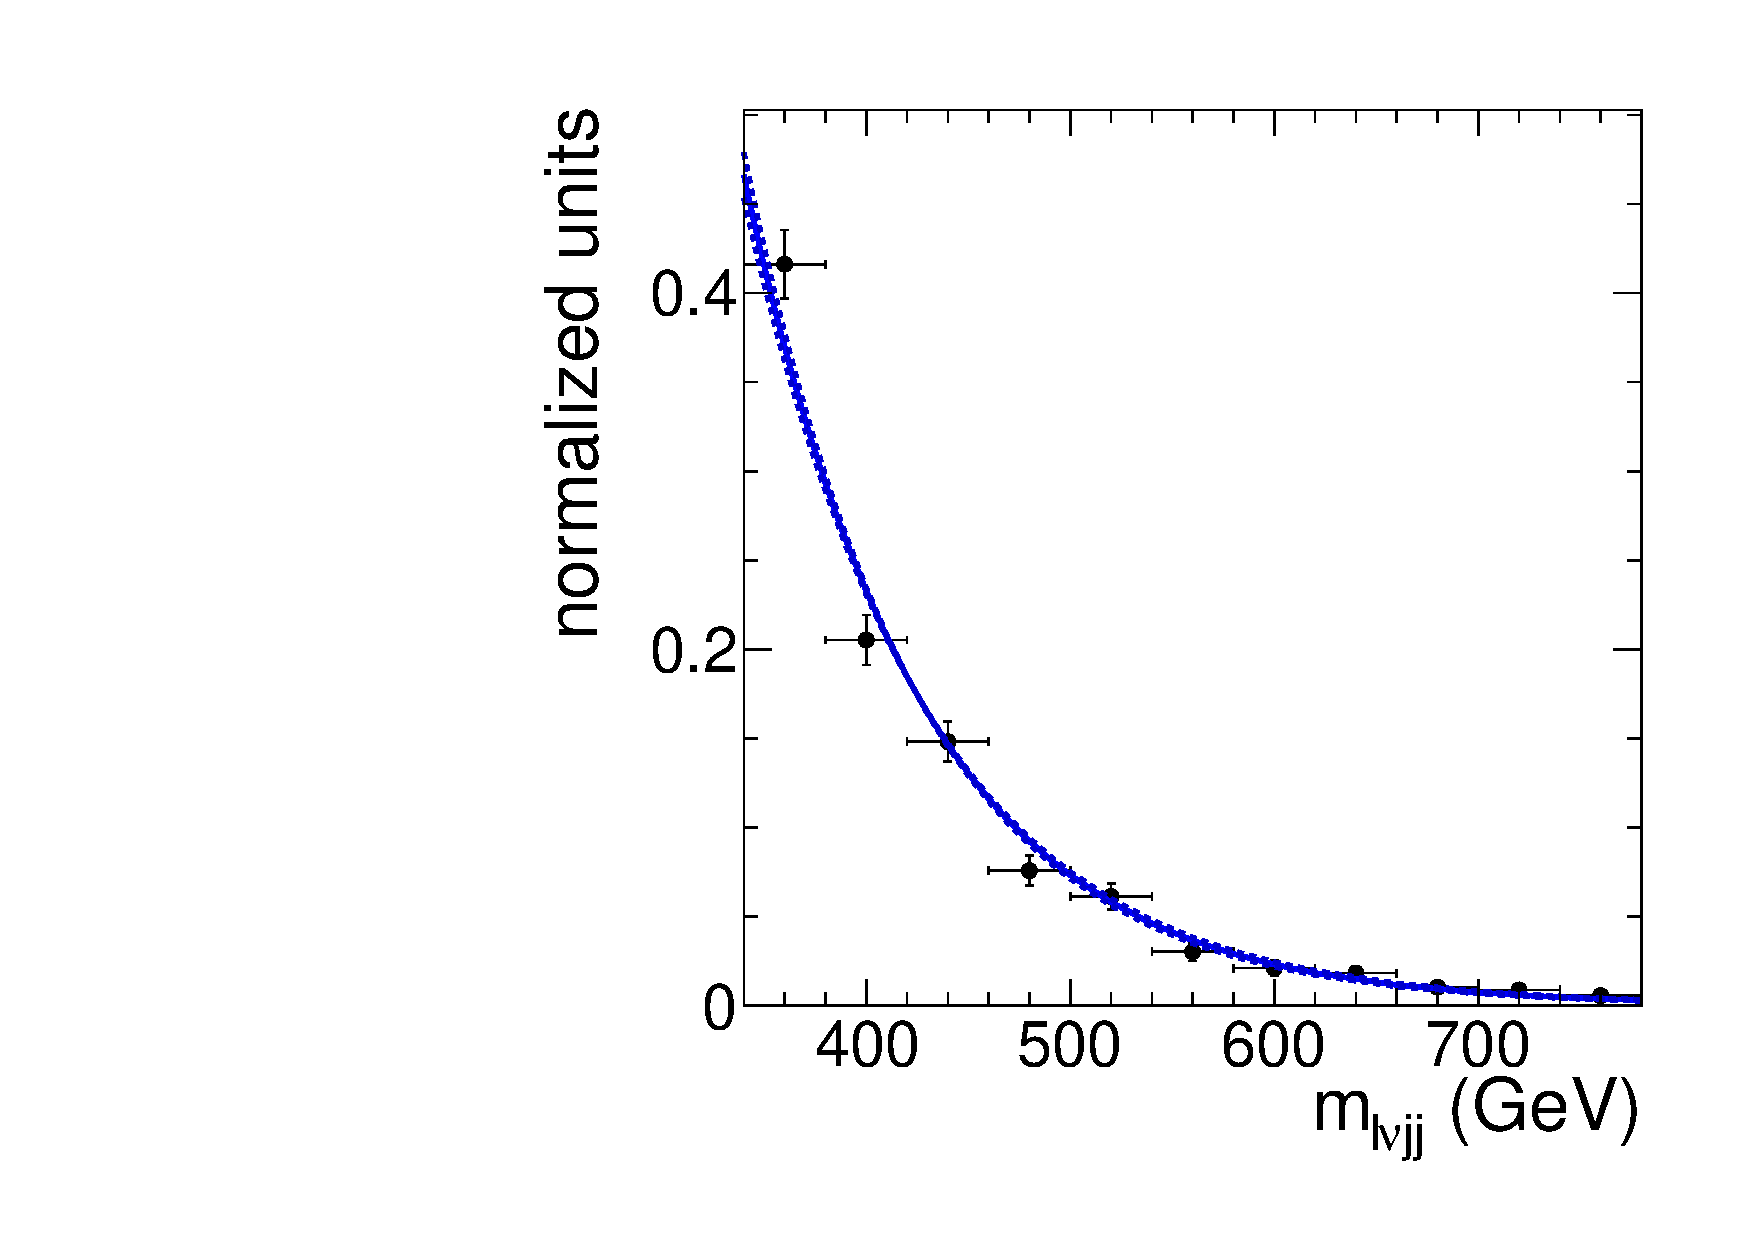
\includegraphics[width=0.49\textwidth]{plots/2012_WJetsShape/H500_Mlvjj_Electron_2jets_WpJShape.pdf}
    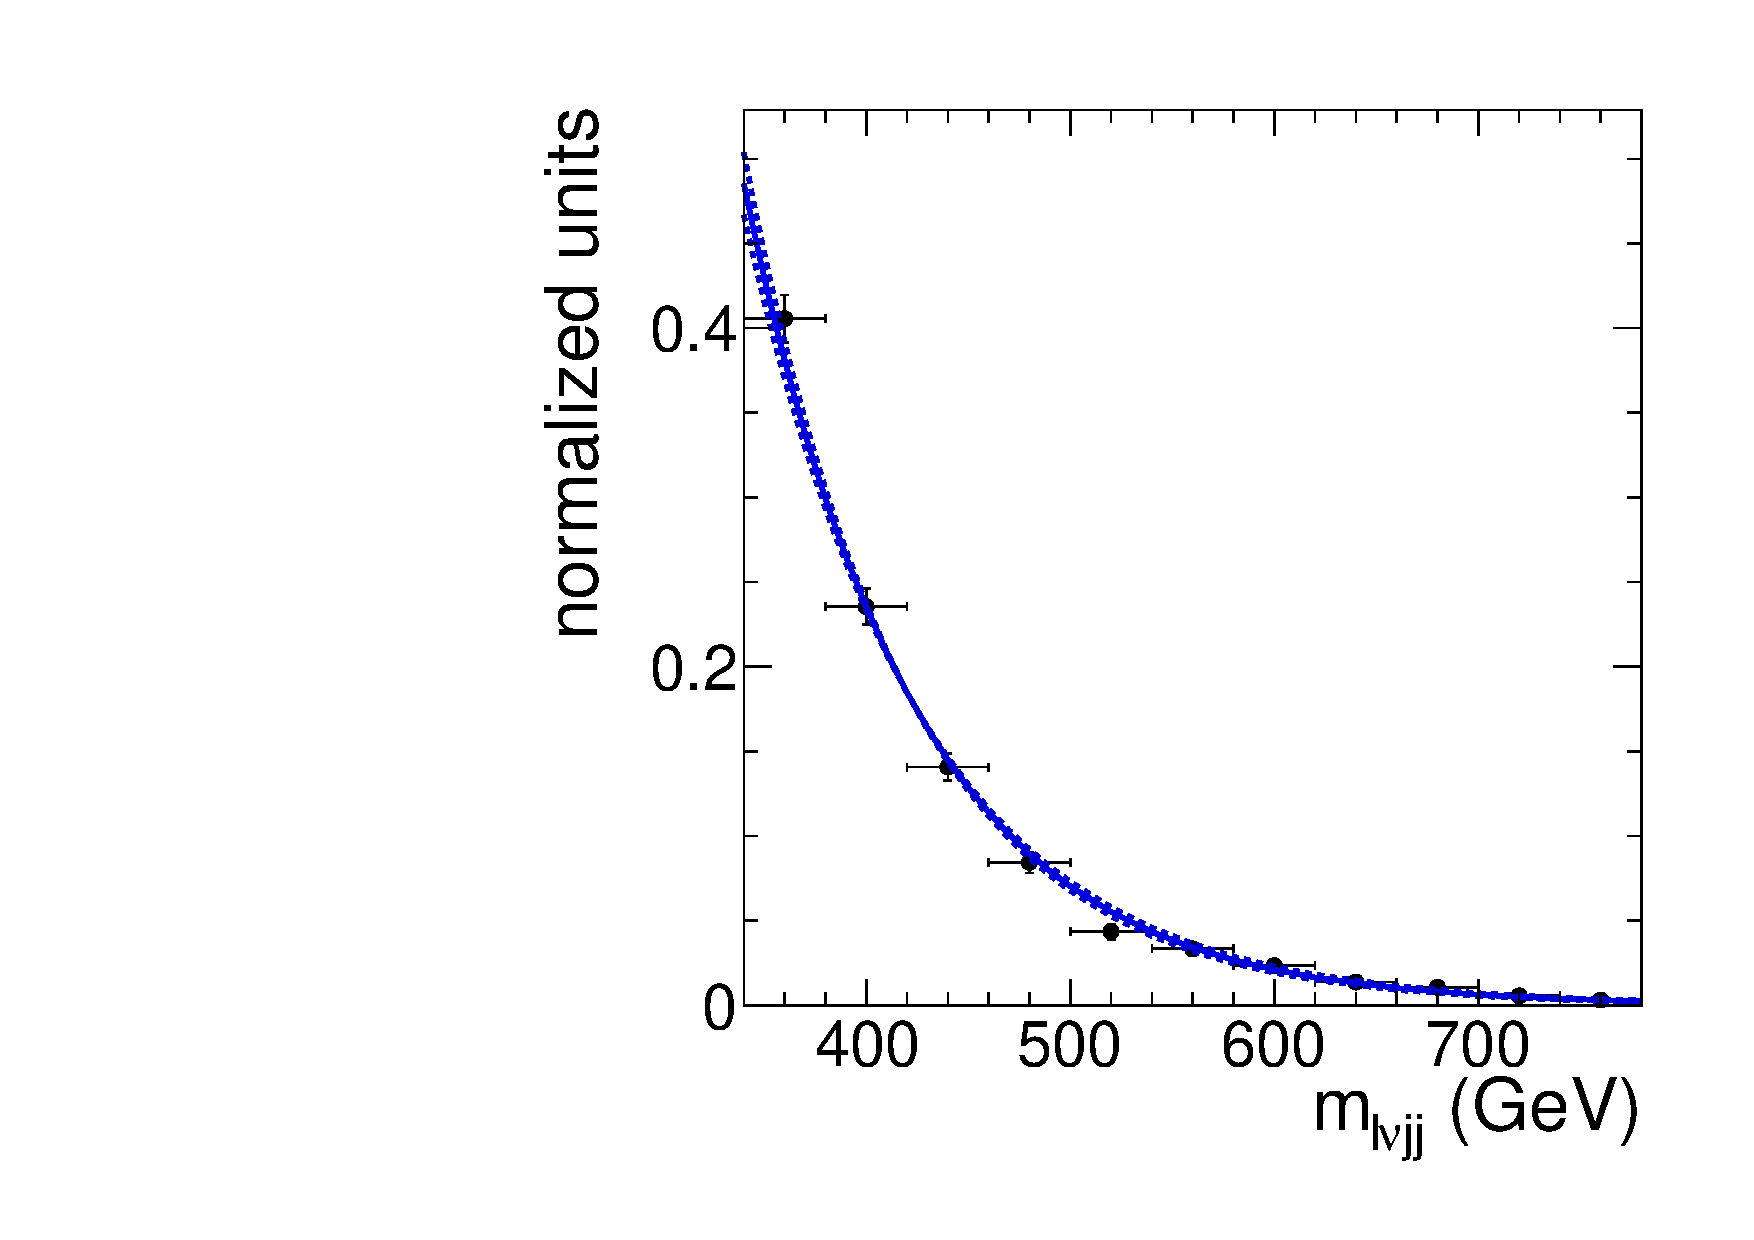
\includegraphics[width=0.49\textwidth]{plots/2012_WJetsShape/H500_Mlvjj_Muon_2jets_WpJShape.pdf}
    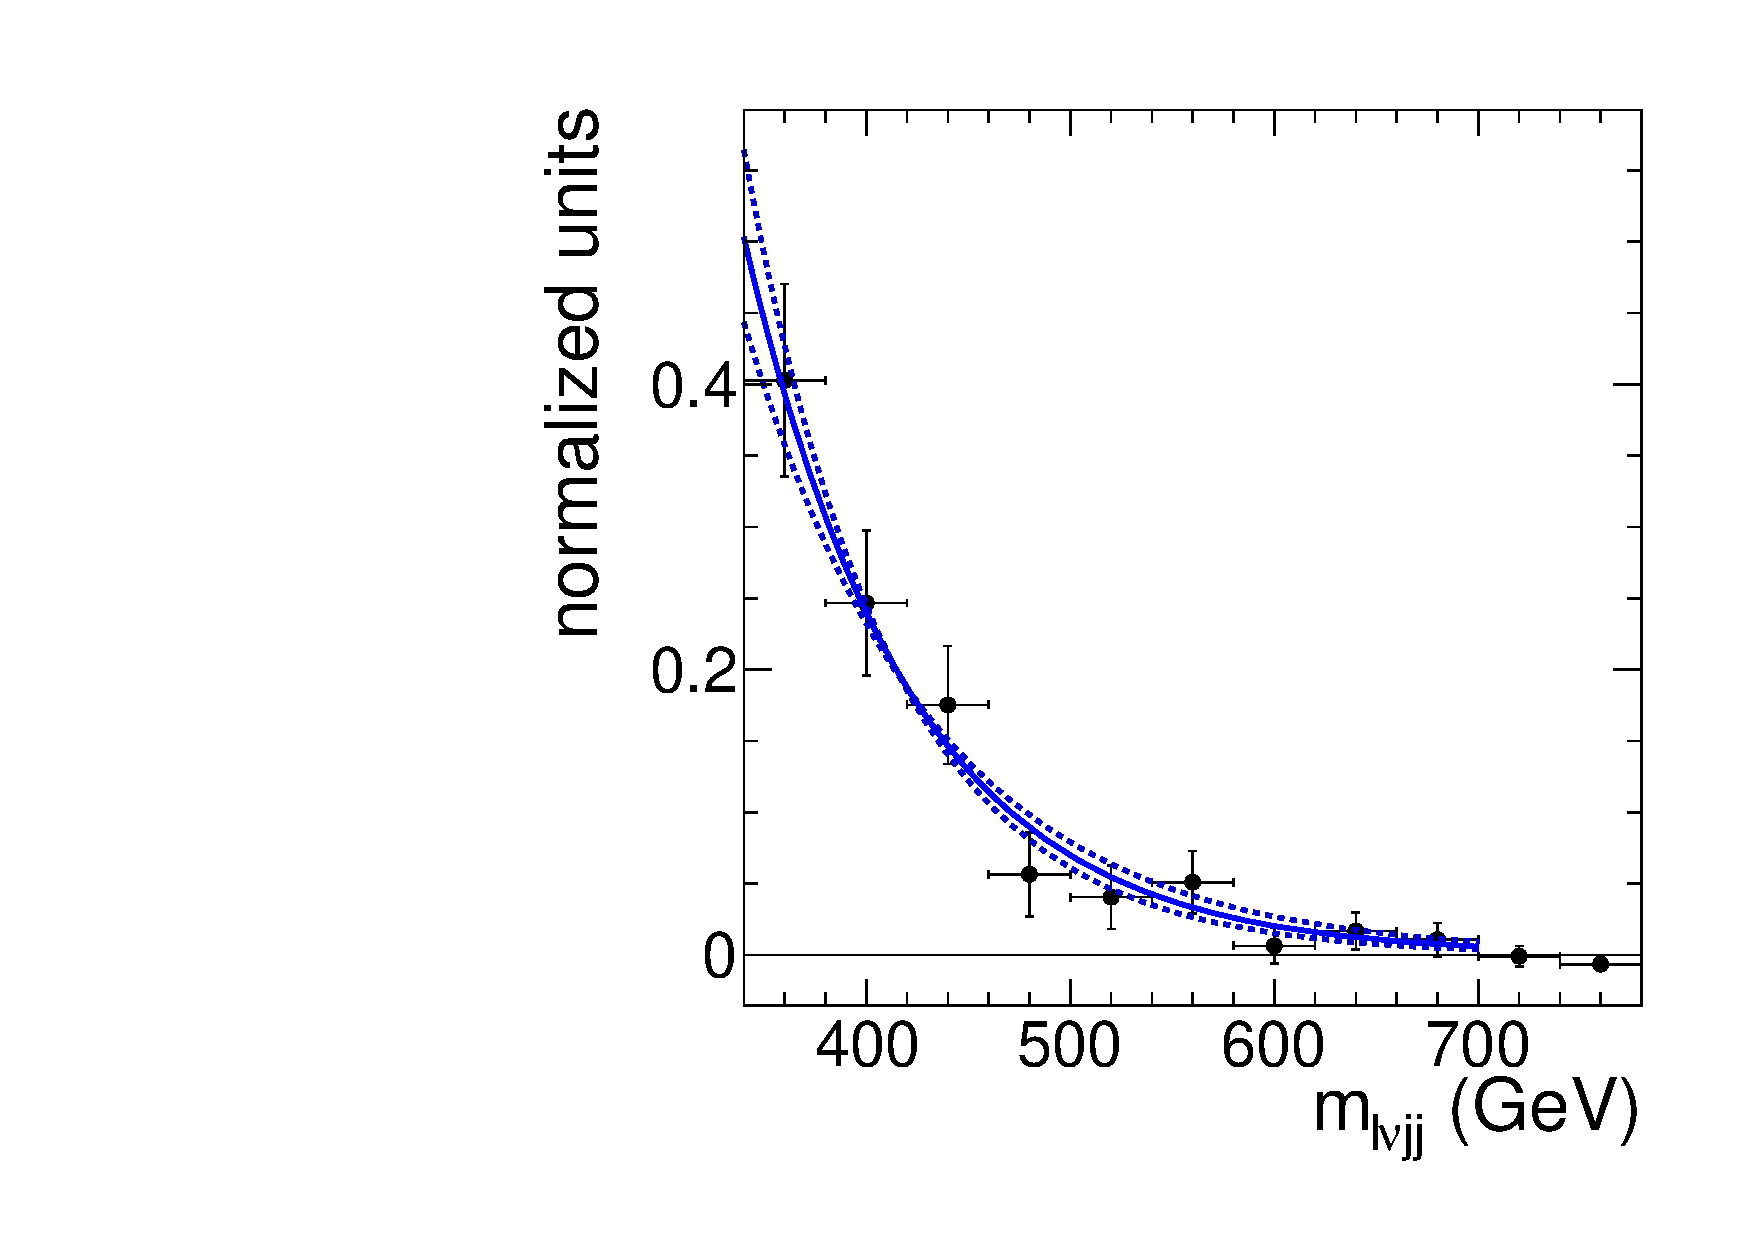
\includegraphics[width=0.49\textwidth]{plots/2012_WJetsShape/H500_Mlvjj_Electron_3jets_WpJShape.pdf}
    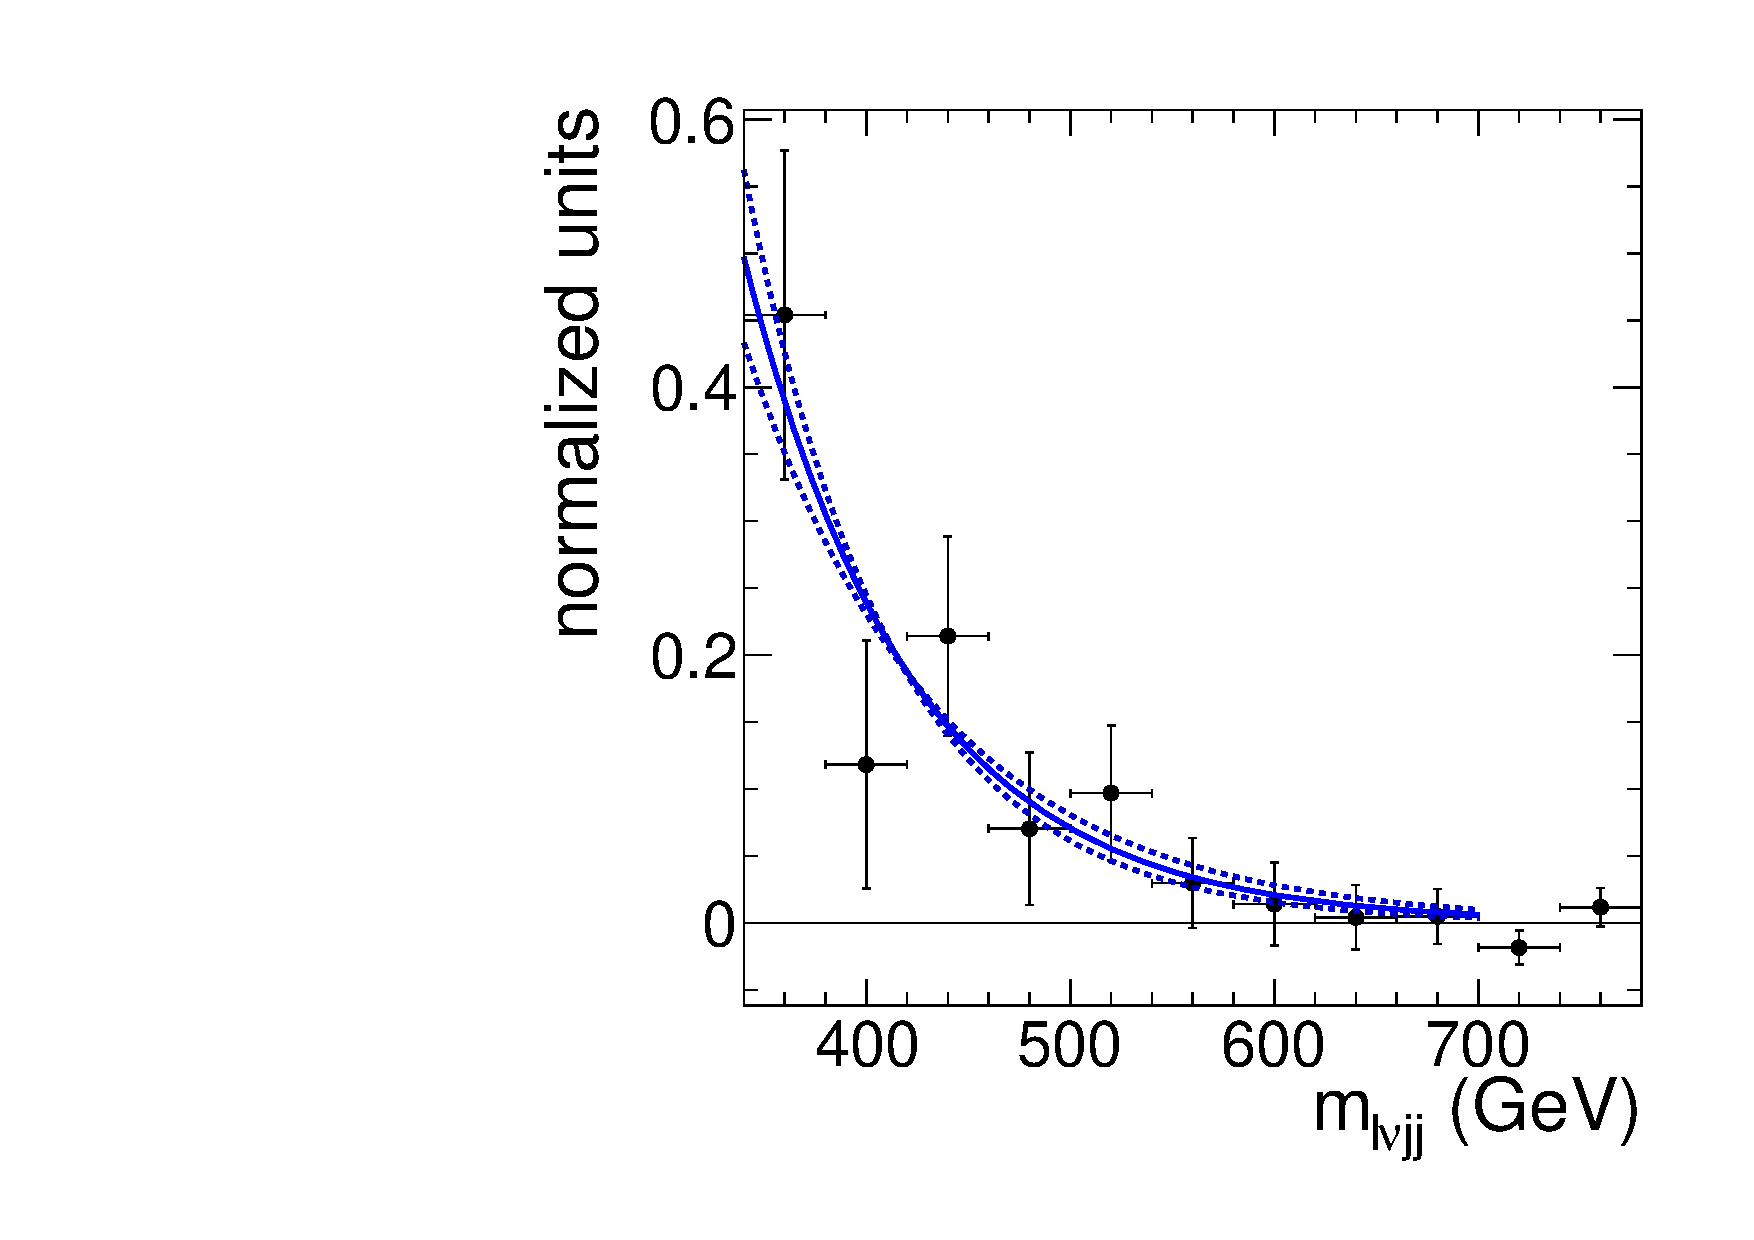
\includegraphics[width=0.49\textwidth]{plots/2012_WJetsShape/H500_Mlvjj_Muon_3jets_WpJShape.pdf}
  \caption{\label{fig:Wjets_dd_500}
  The distribution of the extrapolated background in the signal region
  is reported for the Higgs mass hypothesis of 500 GeV.
  On the top the 2 jets case, on the bottom the 3 jets case.
  Electrons are on the left, muons on the right.
  The points represent the extrapolated points, 
  while the red line shows the fitting function and the blue shaded band 
  the error from the fit.
    } 
\end{figure}
%
\begin{figure}[!t]
  \centering
    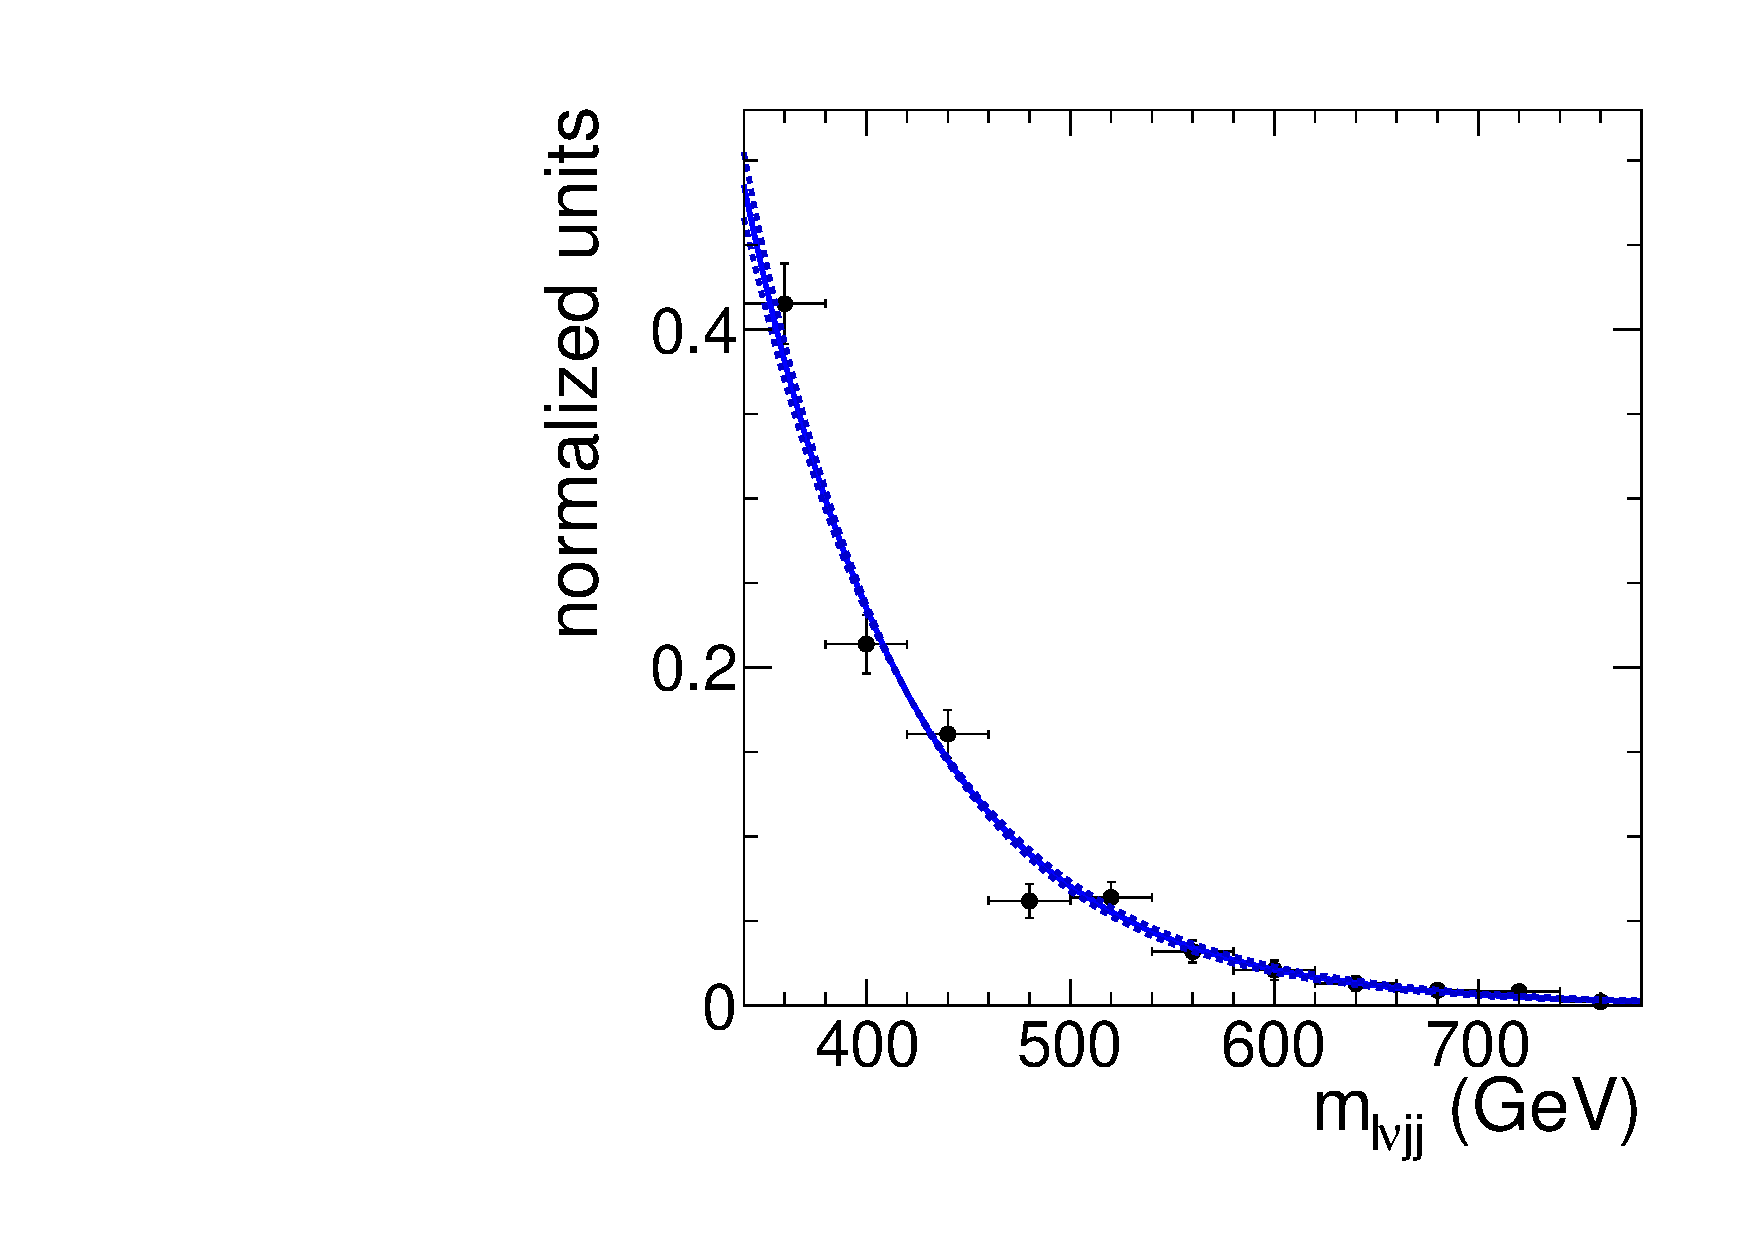
\includegraphics[width=0.49\textwidth]{plots/2012_WJetsShape/H550_Mlvjj_Electron_2jets_WpJShape.pdf}
    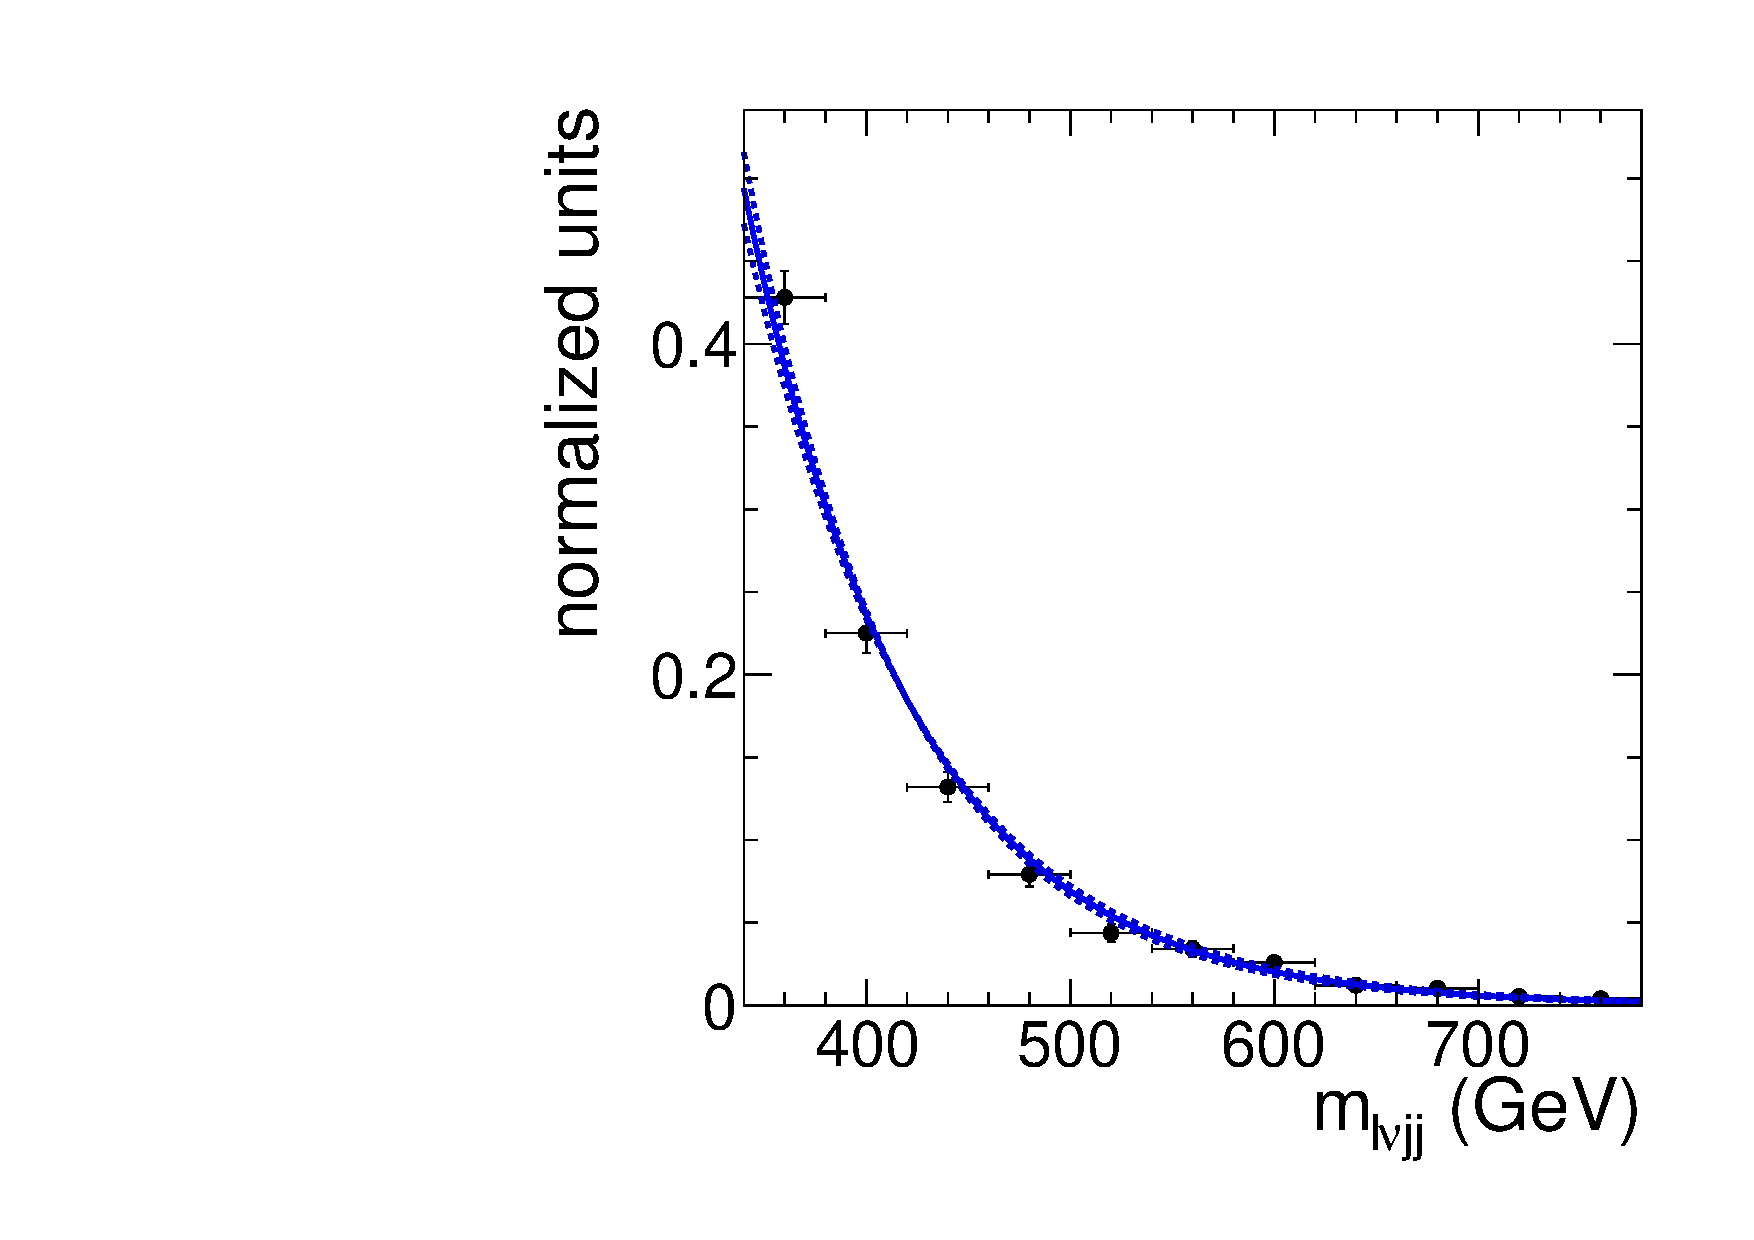
\includegraphics[width=0.49\textwidth]{plots/2012_WJetsShape/H550_Mlvjj_Muon_2jets_WpJShape.pdf}
    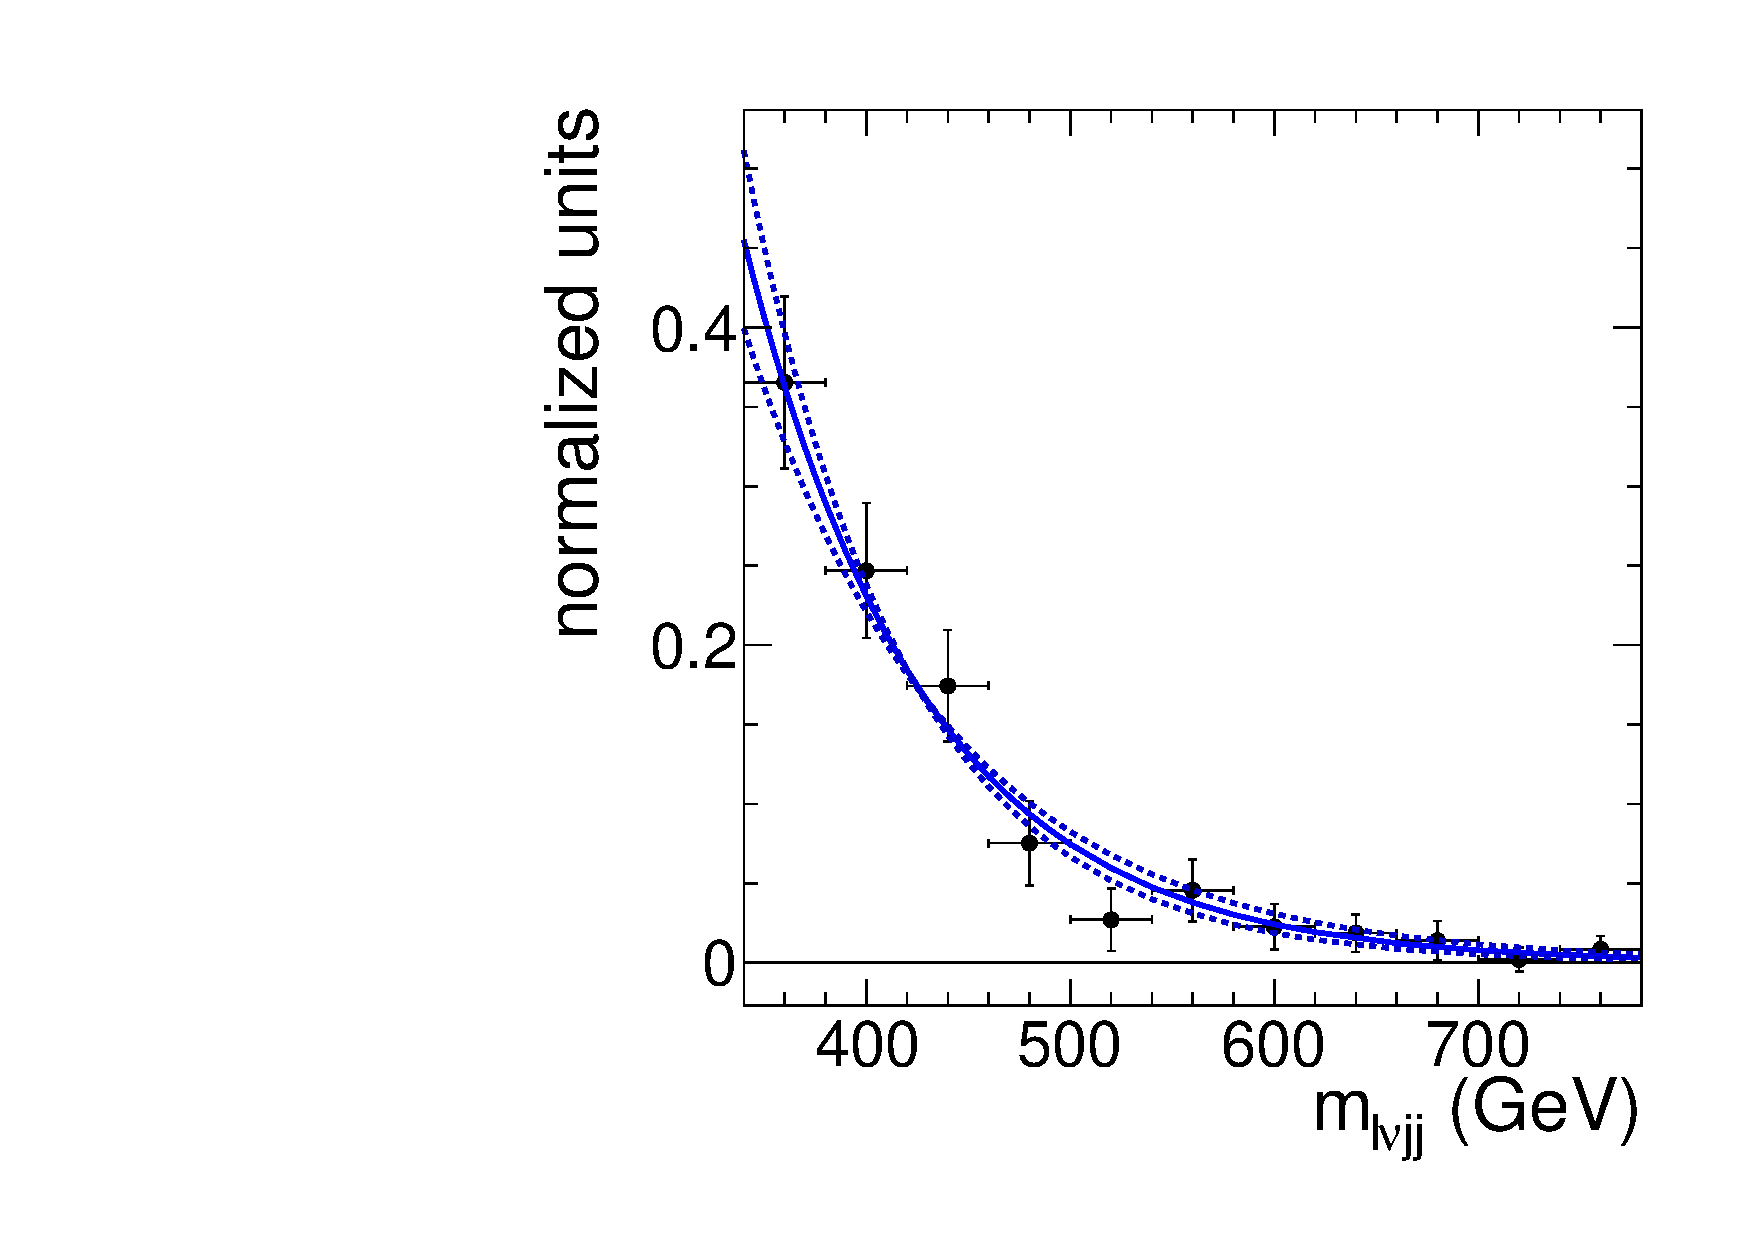
\includegraphics[width=0.49\textwidth]{plots/2012_WJetsShape/H550_Mlvjj_Electron_3jets_WpJShape.pdf}
    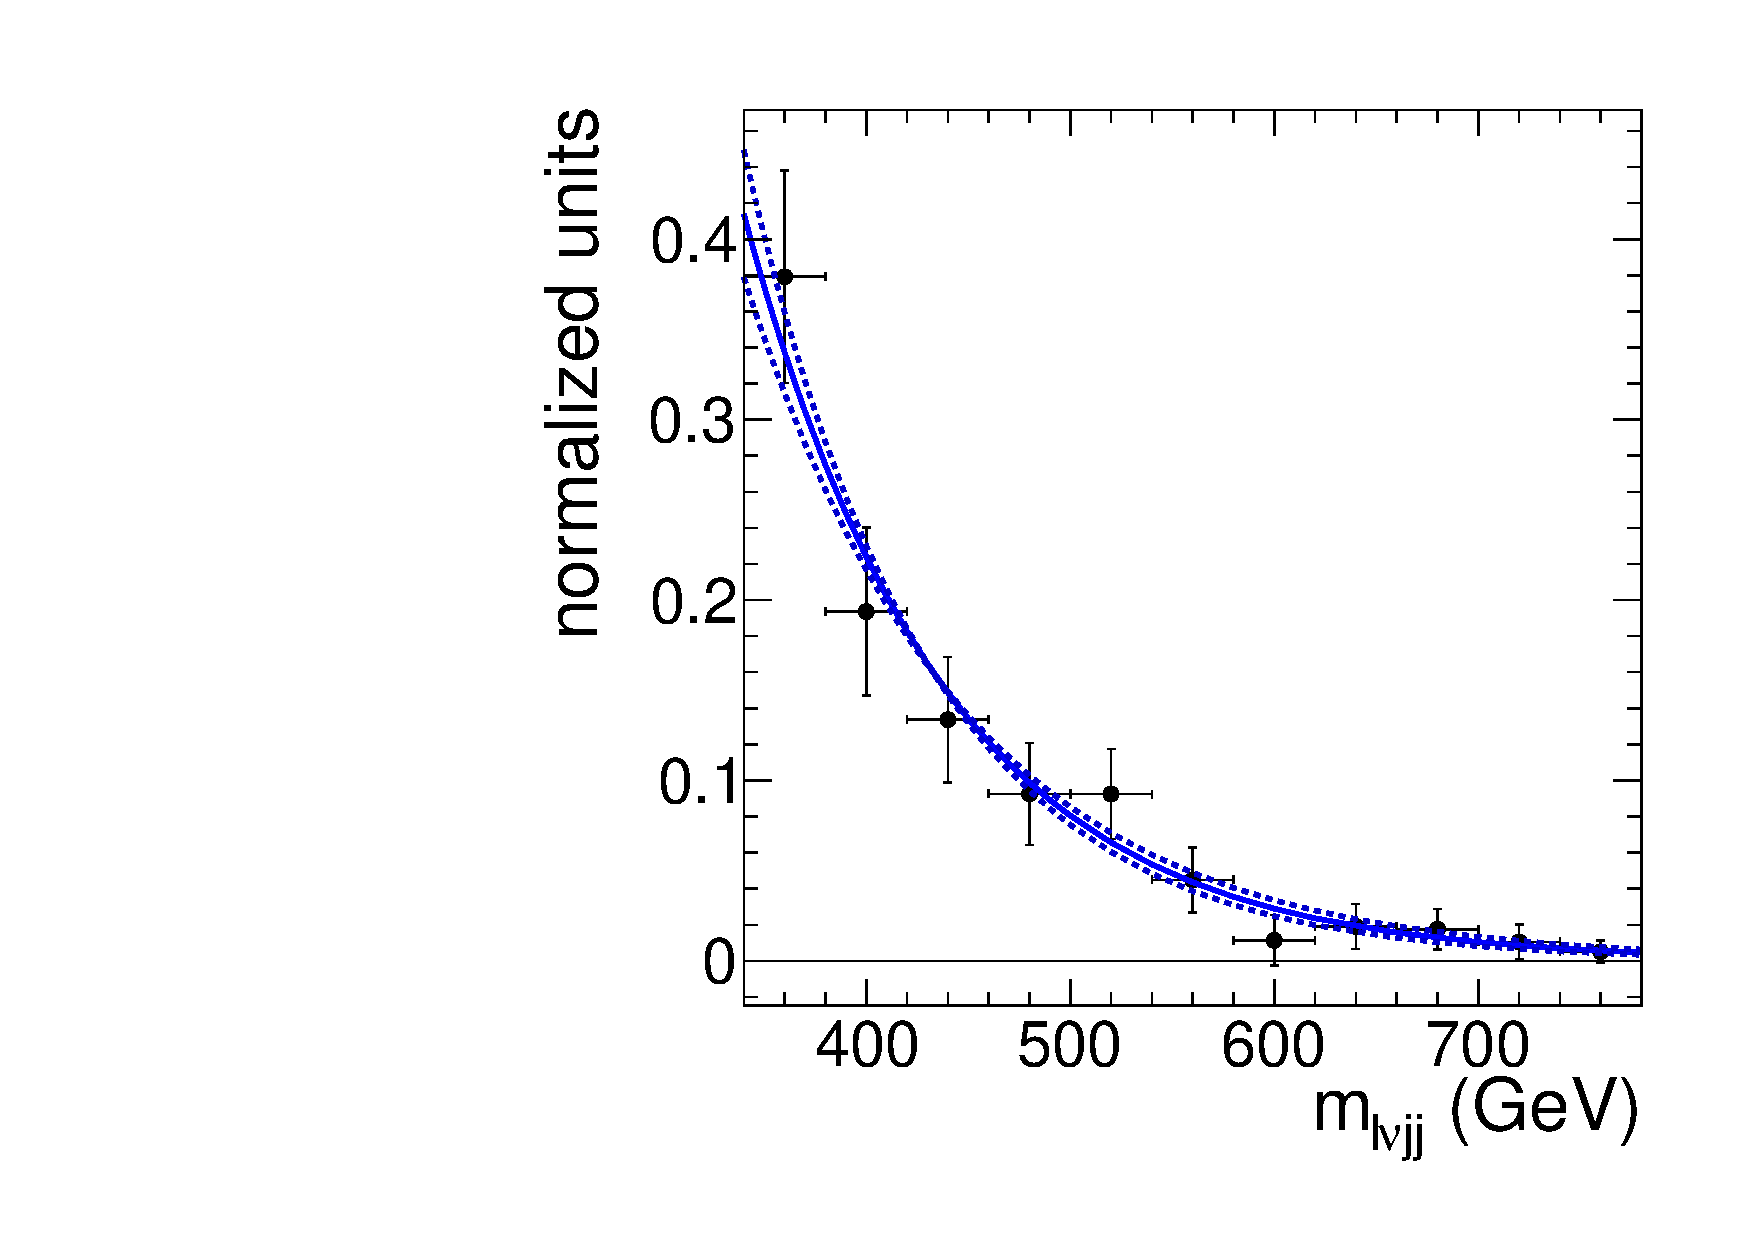
\includegraphics[width=0.49\textwidth]{plots/2012_WJetsShape/H550_Mlvjj_Muon_3jets_WpJShape.pdf}
  \caption{\label{fig:Wjets_dd_550}
  The distribution of the extrapolated background in the signal region
  is reported for the Higgs mass hypothesis of 550 GeV.
  On the top the 2 jets case, on the bottom the 3 jets case.
  Electrons are on the left, muons on the right.
  The points represent the extrapolated points, 
  while the red line shows the fitting function and the blue shaded band 
  the error from the fit.
    } 
\end{figure}
%
\begin{figure}[!t]
  \centering
    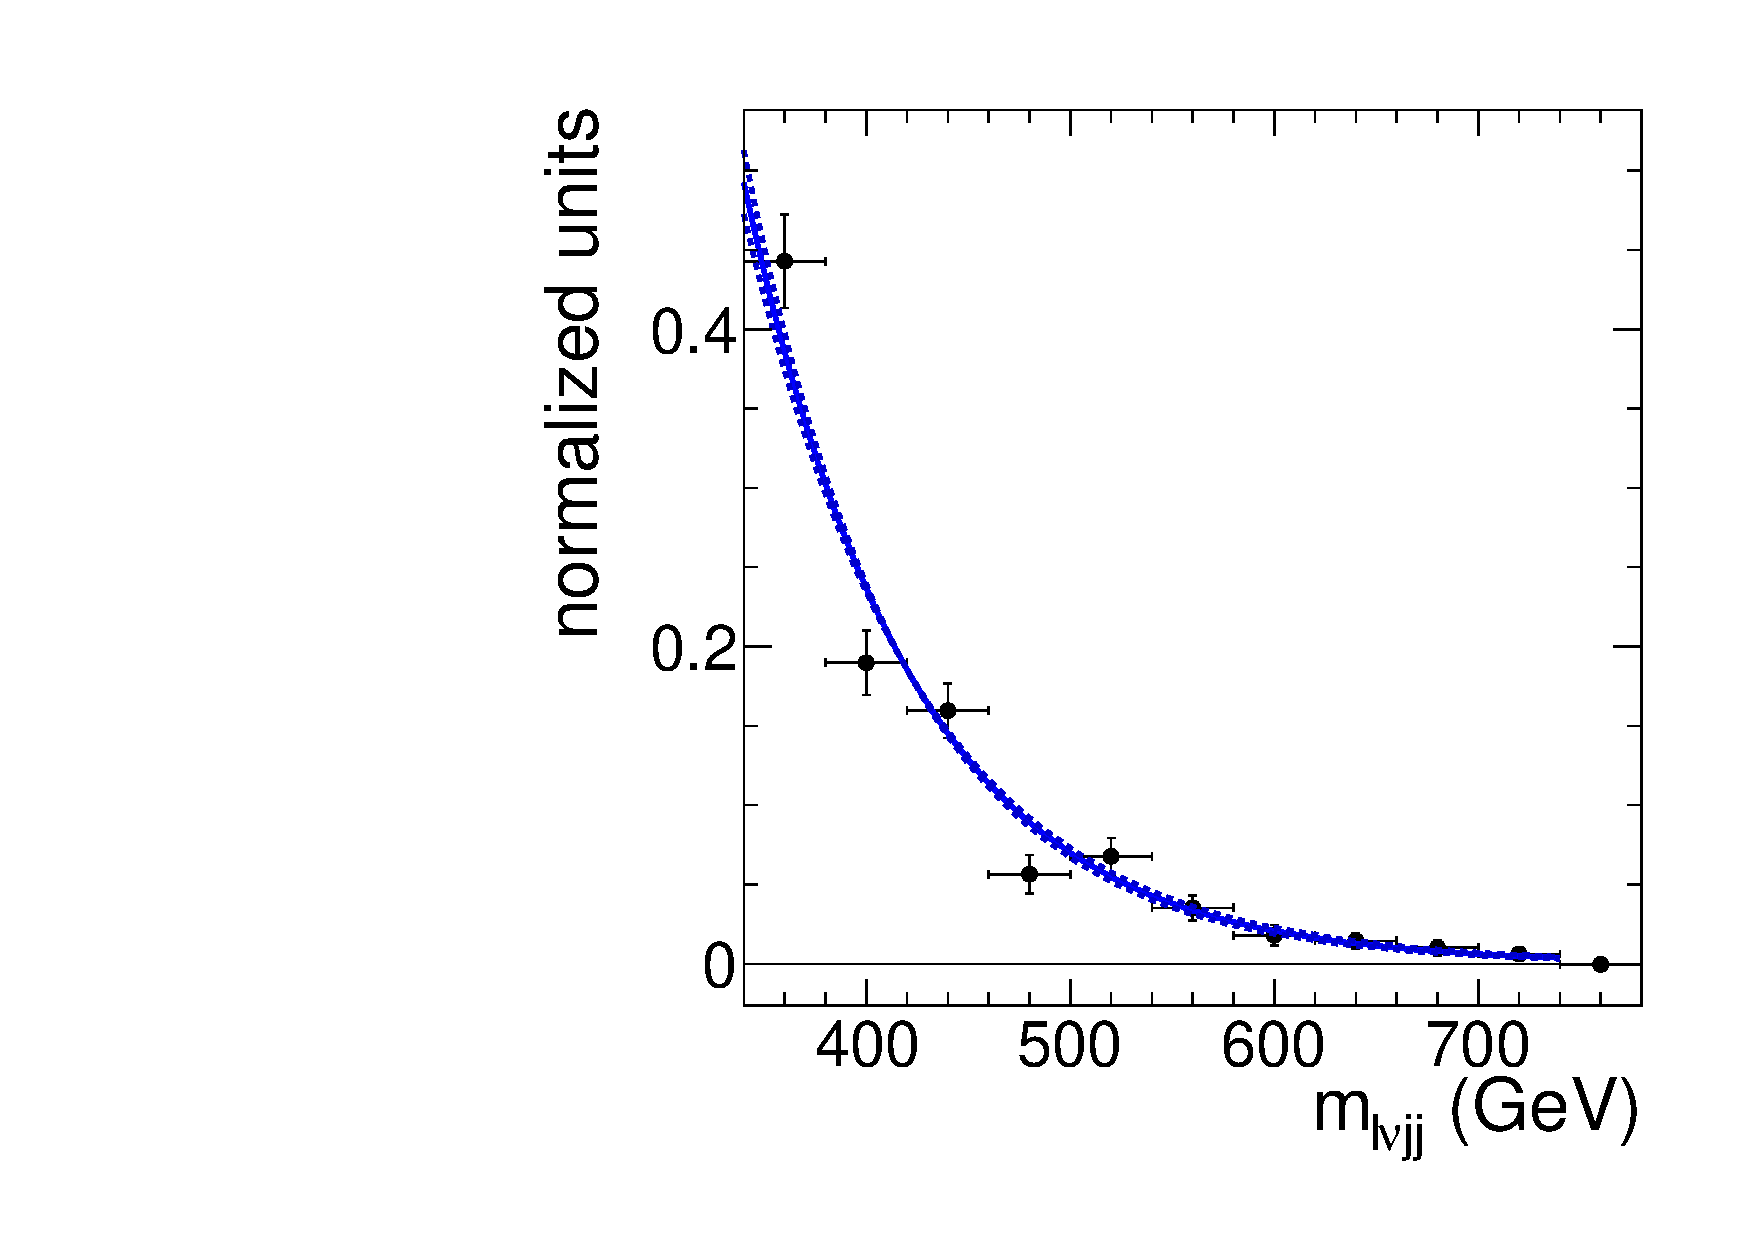
\includegraphics[width=0.49\textwidth]{plots/2012_WJetsShape/H600_Mlvjj_Electron_2jets_WpJShape.pdf}
    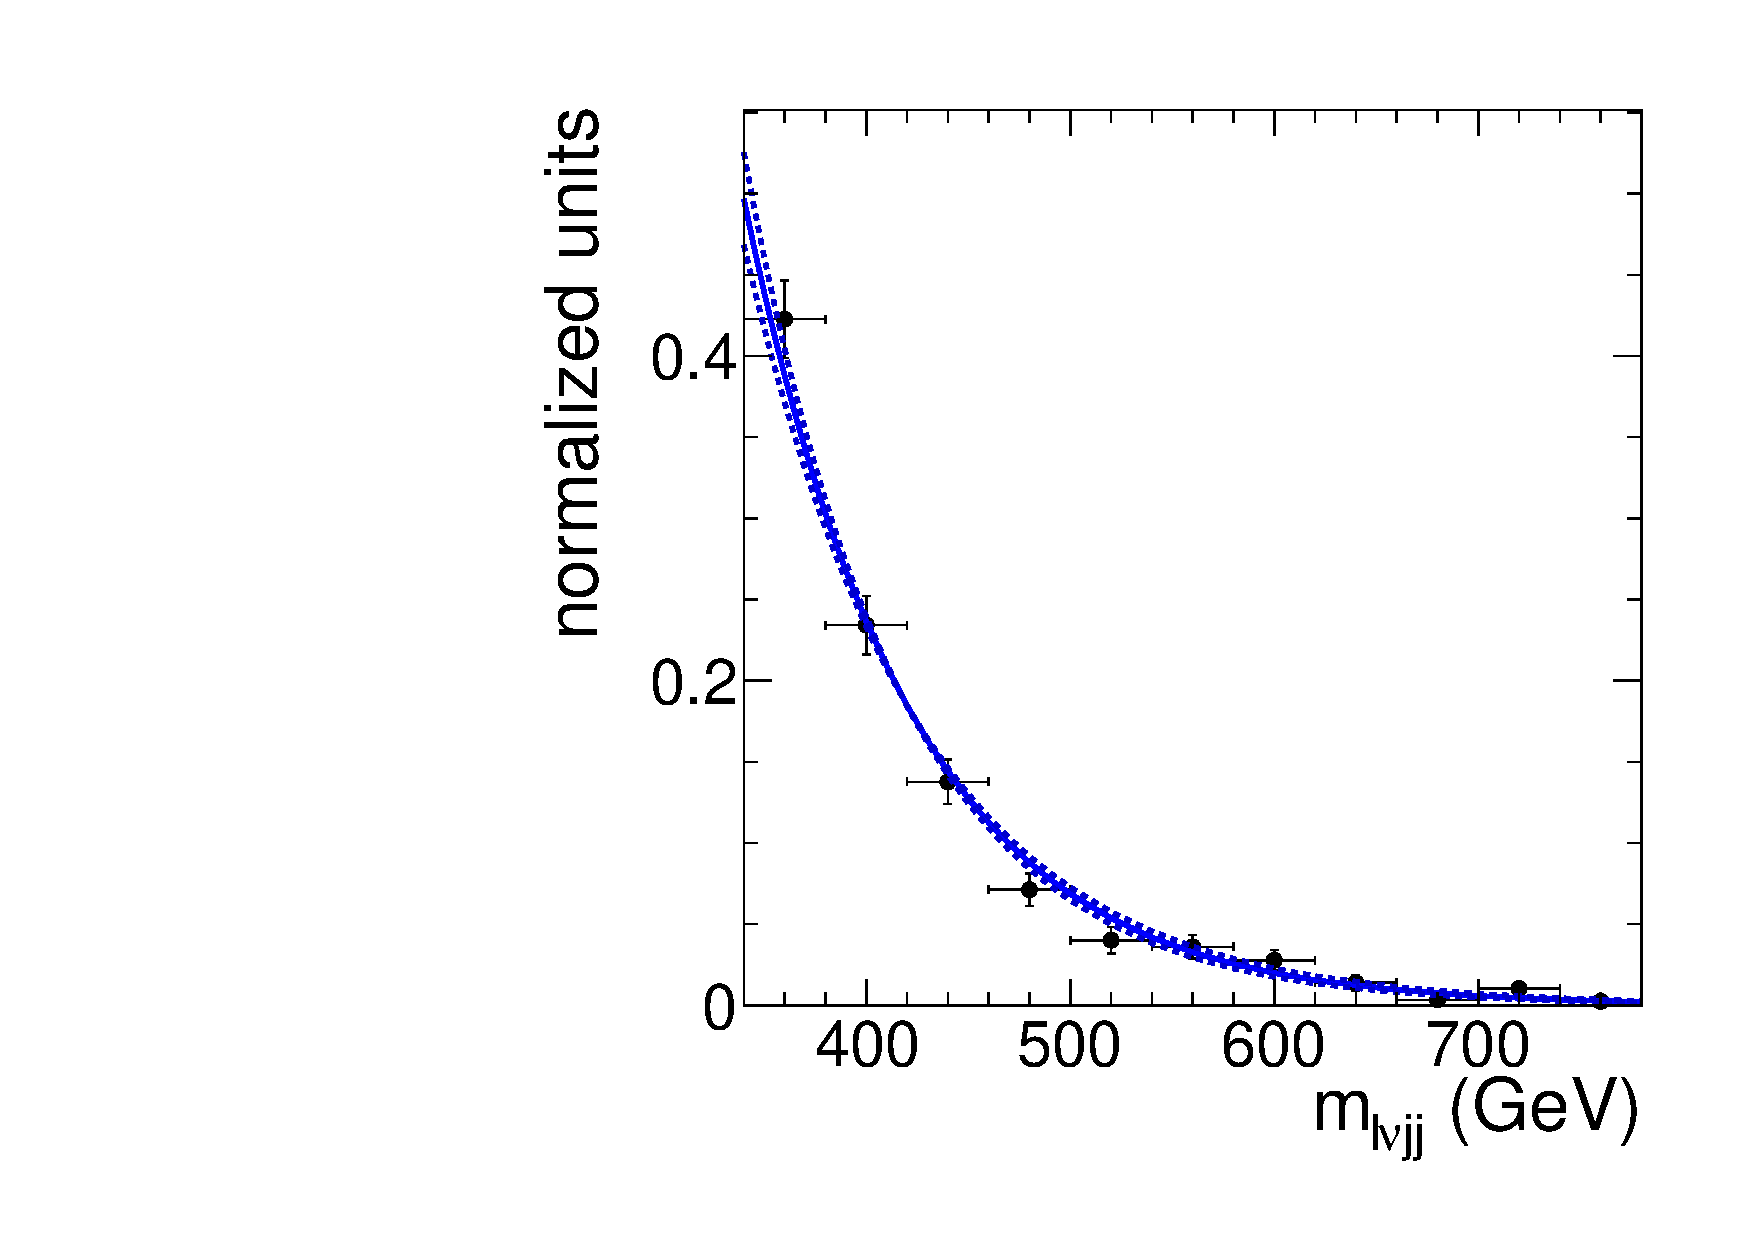
\includegraphics[width=0.49\textwidth]{plots/2012_WJetsShape/H600_Mlvjj_Muon_2jets_WpJShape.pdf}
    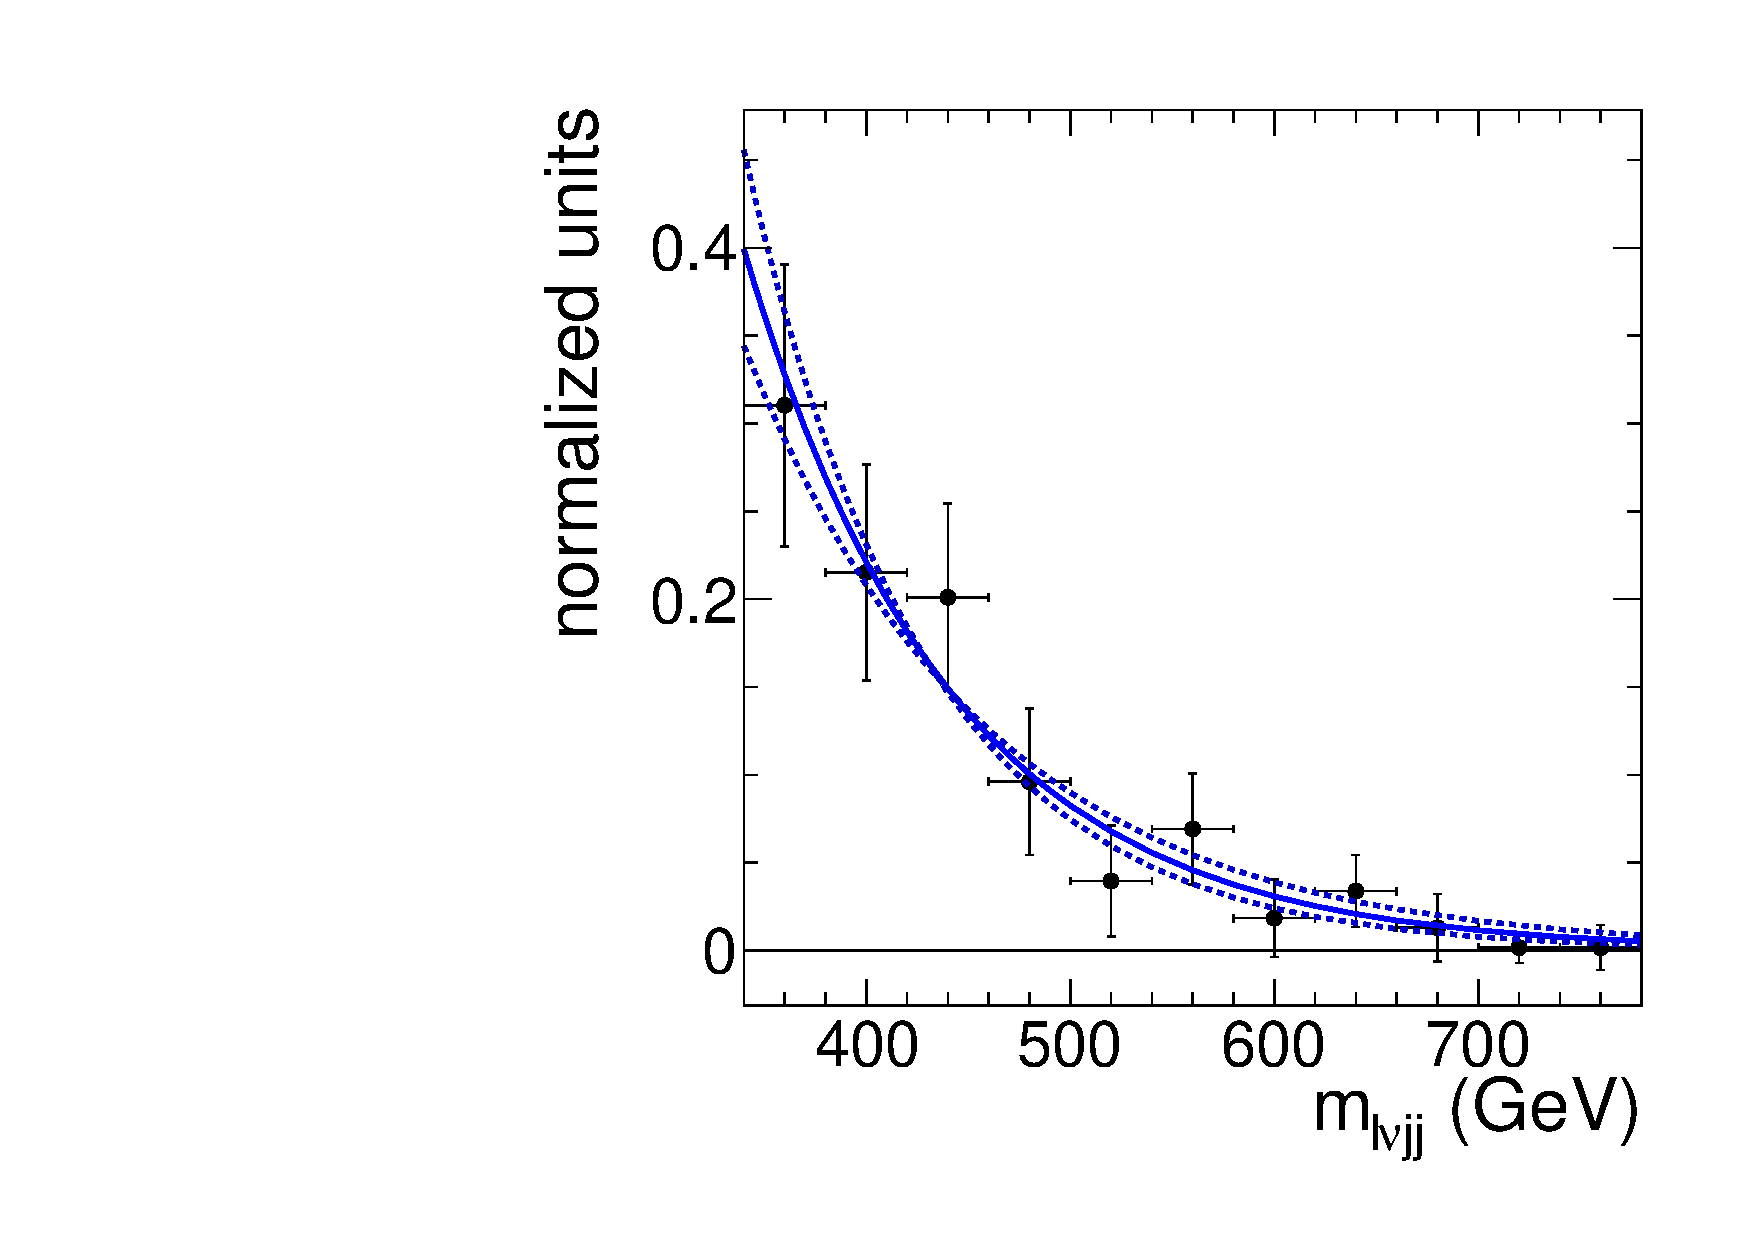
\includegraphics[width=0.49\textwidth]{plots/2012_WJetsShape/H600_Mlvjj_Electron_3jets_WpJShape.pdf}
    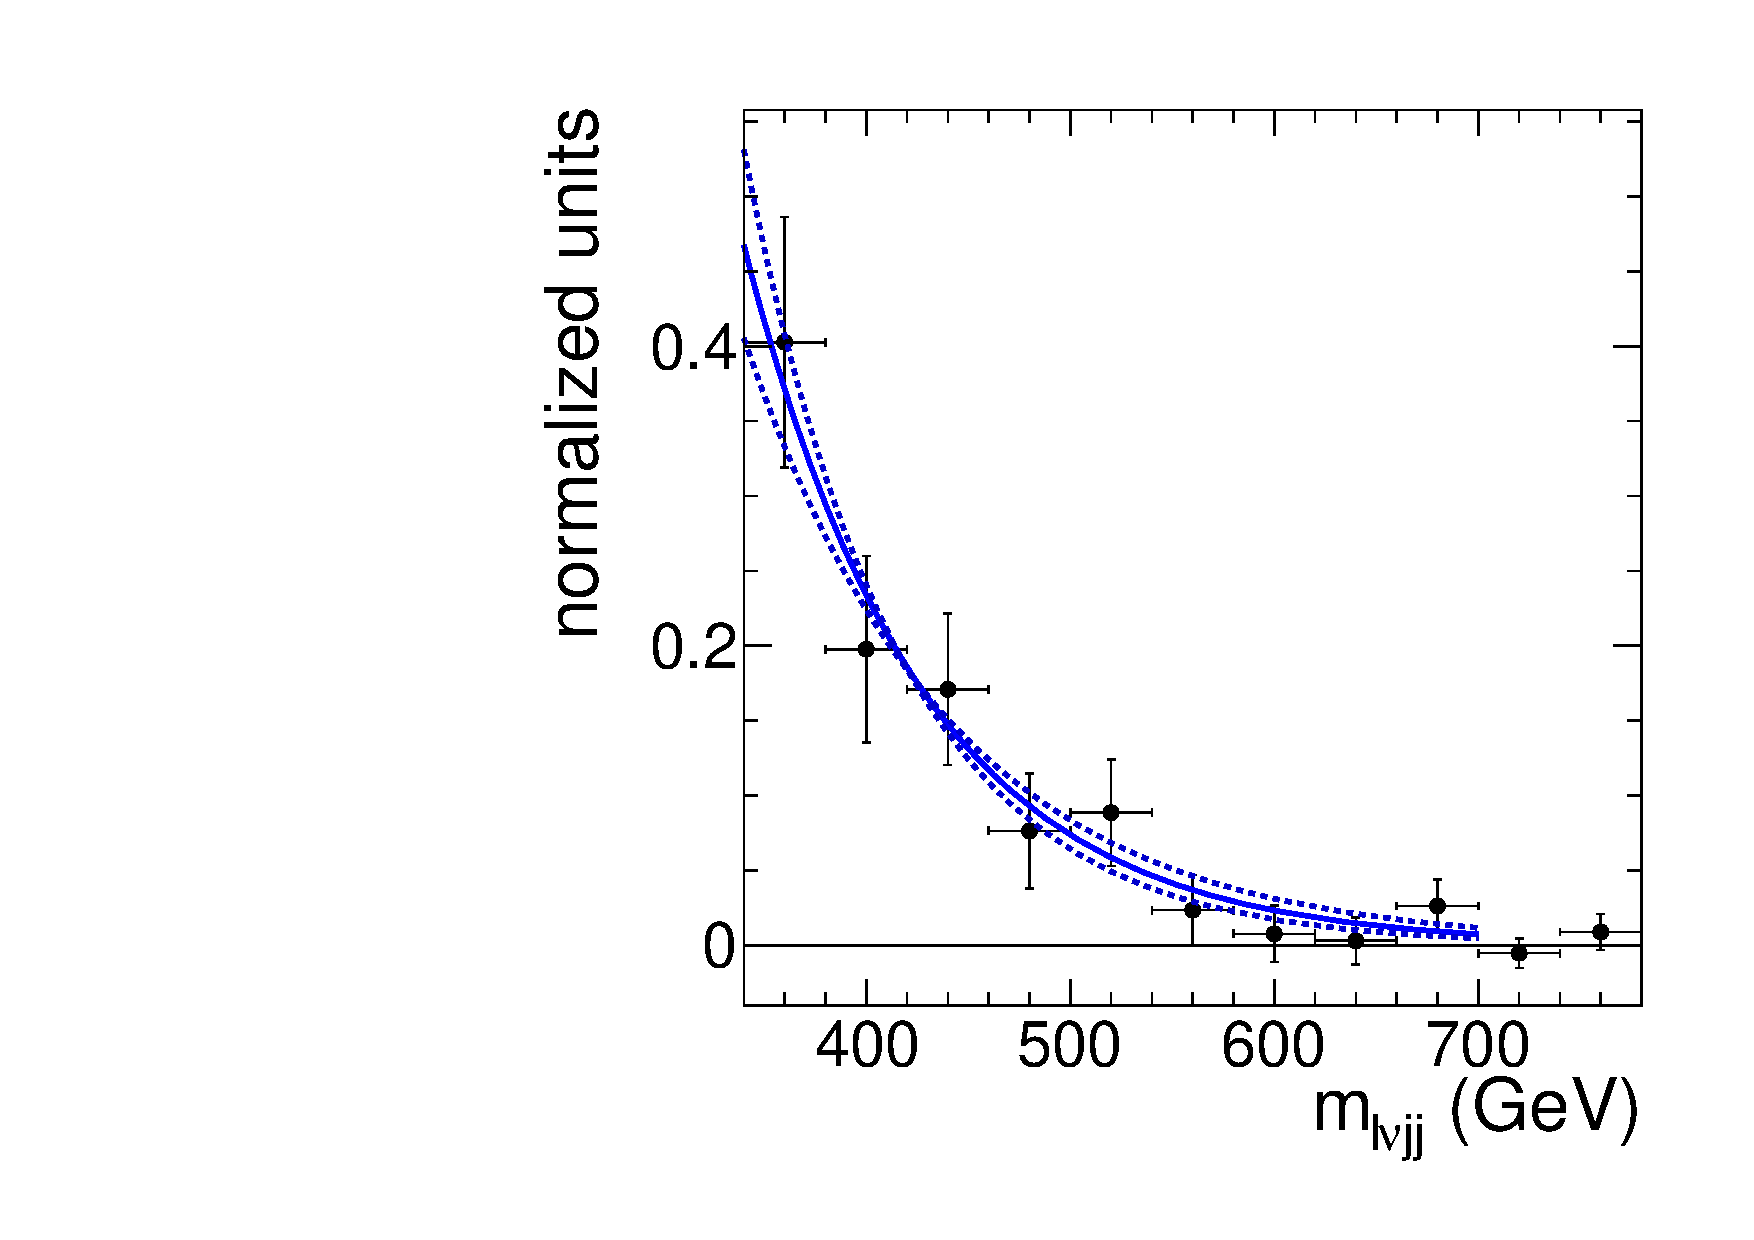
\includegraphics[width=0.49\textwidth]{plots/2012_WJetsShape/H600_Mlvjj_Muon_3jets_WpJShape.pdf}
  \caption{\label{fig:Wjets_dd_600}
  The distribution of the extrapolated background in the signal region
  is reported for the Higgs mass hypothesis of 600 GeV.
  On the top the 2 jets case, on the bottom the 3 jets case.
  Electrons are on the left, muons on the right.
  The points represent the extrapolated points, 
  while the red line shows the fitting function and the blue shaded band 
  the error from the fit.
    } 
\end{figure}
